
\apendice{Resultados estudio}

\section{Introducción}

En este apartado se detallaran las pruebas realizadas durante el desarrollo de la aplicación para mostrar su funcion.

\section{Comparativa de algoritmos}

Tras la optimización del algoritmo pero antes de la implementación a la pagina web, se buscó comparar el funcionamiento y los resultados que podían proporcionar los diferentes algoritmos de clustering bajo condiciones relativamente equivalentes. Para ello, se utilizó la misma cantidad de datos: doscientas filas del archivo \texttt{Trayectorias Taxis} \cite{trayectorias_taxis}. Respecto a los parámetros necesarios para la ejecución de cada algoritmo, se intentó mantenerlos lo más estándar posible. Por ejemplo, en los casos en que era necesario especificar el número de clusters, se utilizó una aproximación basada en el resultado obtenido por OPTICS, ya que este algoritmo no requiere definir dicho parámetro. El resto de los parámetros se dejaron en los valores predeterminados que proporciona la biblioteca \texttt{scikit-learn}.

Aunque se probaron más algoritmos, solo cinco llegaron a la etapa final del desarrollo de la página web. Algunos, como \textbf{Birch}, no lograron producir resultados satisfactorios, aunque se considera que, con una adaptación más específica de los datos, podrían haber funcionado correctamente.

A continuación, se describen los resultados obtenidos para cada uno de los algoritmos seleccionados:

\begin{enumerate}

\item \textbf{OPTICS}:  
Este fue el primer algoritmo probado de manera intensiva, ya que era el utilizado por defecto en la implementación base. De las doscientas filas procesadas, se generaron un total de 2161 segmentos, que fueron agrupados en 106 clusters. Sin embargo, no todos los segmentos se utilizaron para la creación de los clusters; un total de 1354 segmentos fueron catalogados como "basura", lo que corresponde al 62.66\% de los datos. A continuación, se muestran los resultados en tres imágenes diferentes: la representación de los clusters, un histograma con la cantidad de trayectorias que forman cada cluster y la representación de trayectorias generadas por el algoritmo TRACLUS.

\begin{figure}[h!]
    \centering
    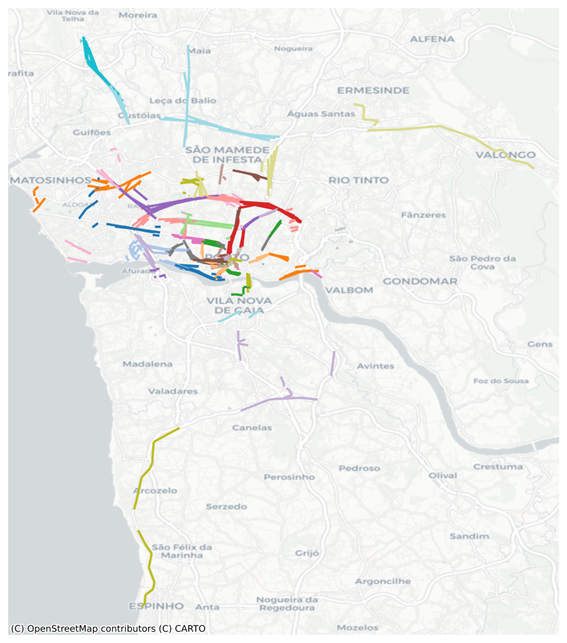
\includegraphics[width=0.5\textwidth]{img/clusters_OPTICS.png}
    \caption{Representación de clusters.}
    \label{fig:clusters_OPTICS}
\end{figure}

\begin{figure}[h!]
    \centering
    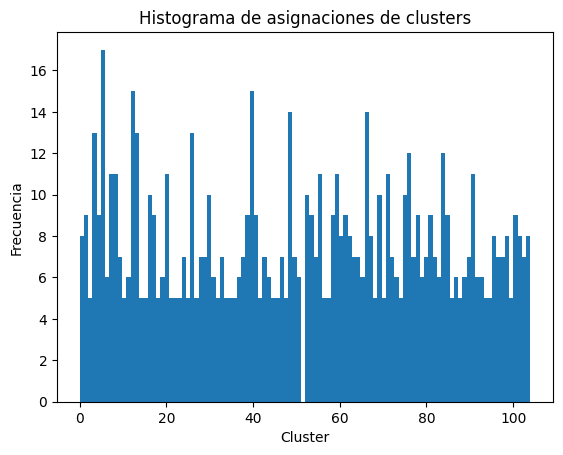
\includegraphics[width=0.5\textwidth]{img/histograma_OPTICS.png}
    \caption{Segmentos por cada cluster.}
    \label{fig:histograma_OPTICS}
\end{figure}

\begin{figure}[h!]
    \centering
    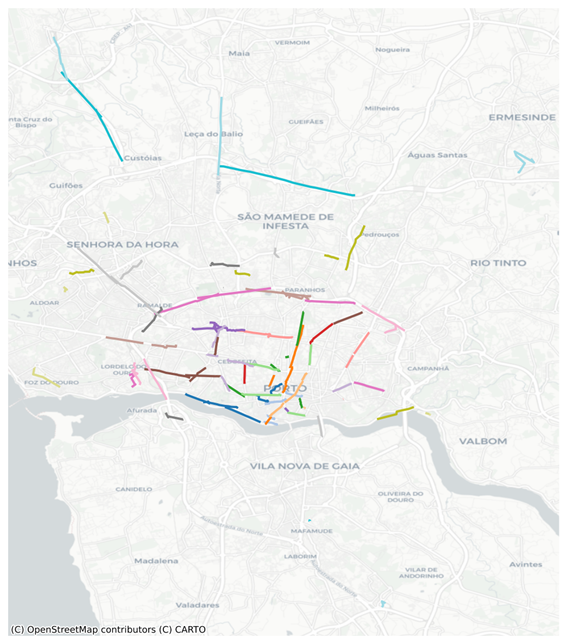
\includegraphics[width=0.5\textwidth]{img/r_tray_OPTICS.png}
    \caption{Representación de trayectorias.}
    \label{fig:trayectorias_OPTICS}
\end{figure}

\FloatBarrier

\item \textbf{DBSCAN}:  
Con un valor de \texttt{eps} de 0.1, los resultados de DBSCAN fueron significativamente diferentes a los de OPTICS. Aunque se generaron más segmentos (2654 en total), el número de clusters disminuyó a 37. Además, el porcentaje de datos clasificados como "basura" aumentó al 90.09\%, lo que equivale a 2391 segmentos descartados.

\begin{figure}[h!]
    \centering
    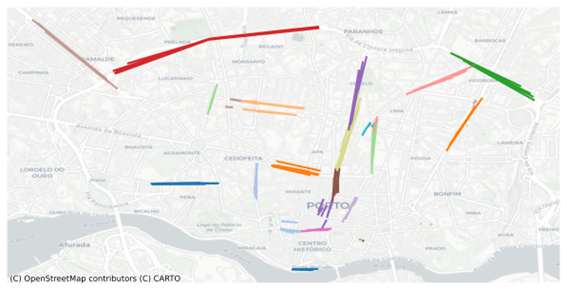
\includegraphics[width=0.5\textwidth]{img/clusters_DBSCAN.png}
    \caption{Representación de clusters.}
    \label{fig:clusters_DBSCAN}
\end{figure}

\begin{figure}[h!]
    \centering
    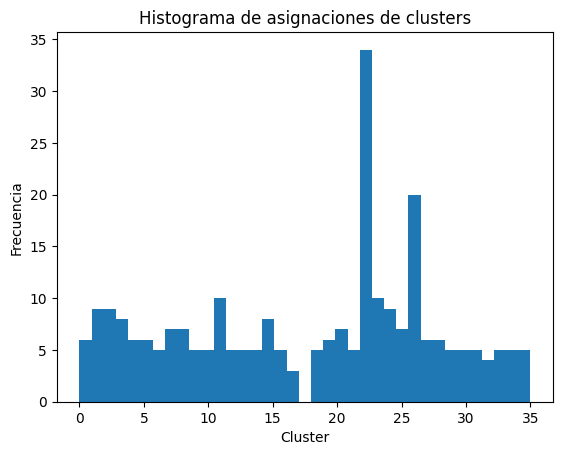
\includegraphics[width=0.5\textwidth]{img/histograma_DBSCAN.png}
    \caption{Segmentos por cada cluster.}
    \label{fig:histograma_DBSCAN}
\end{figure}

\begin{figure}[h!]
    \centering
    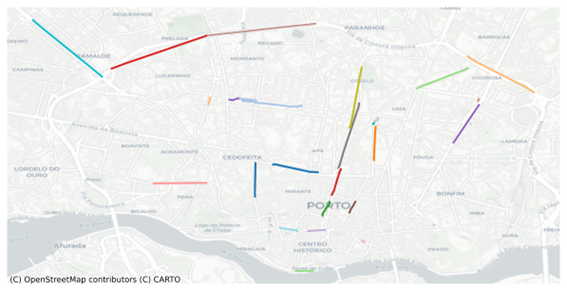
\includegraphics[width=0.5\textwidth]{img/r_tray_DBSCAN.png}
    \caption{Representación de trayectorias.}
    \label{fig:trayectorias_DBSCAN}
\end{figure}

\FloatBarrier

\item \textbf{HDBSCAN}:  
Este algoritmo no requirió ajustes en sus parámetros predeterminados de \texttt{scikit-learn}. Los resultados fueron similares a los de OPTICS en términos de segmentos (2161), aunque el número de clusters fue menor (96) y el porcentaje de segmentos descartados también disminuyó, alcanzando un 53.54\% (1157 segmentos).

\begin{figure}[h!]
    \centering
    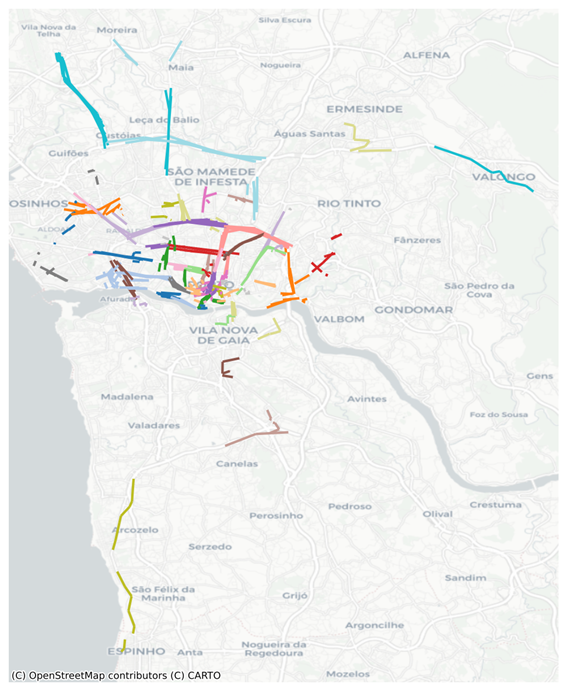
\includegraphics[width=0.5\textwidth]{img/clusters_HDBSCAN.png}
    \caption{Representación de clusters.}
    \label{fig:clusters_HDBSCAN}
\end{figure}

\begin{figure}[h!]
    \centering
    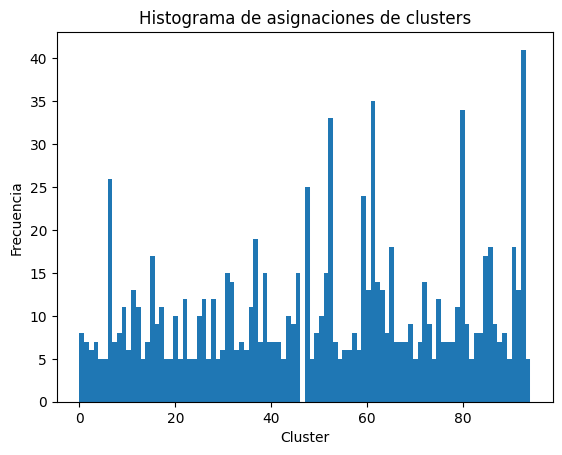
\includegraphics[width=0.5\textwidth]{img/histograma_HDBSCAN.png}
    \caption{Segmentos por cada cluster.}
    \label{fig:histograma_HDBSCAN}
\end{figure}

\begin{figure}[h!]
    \centering
    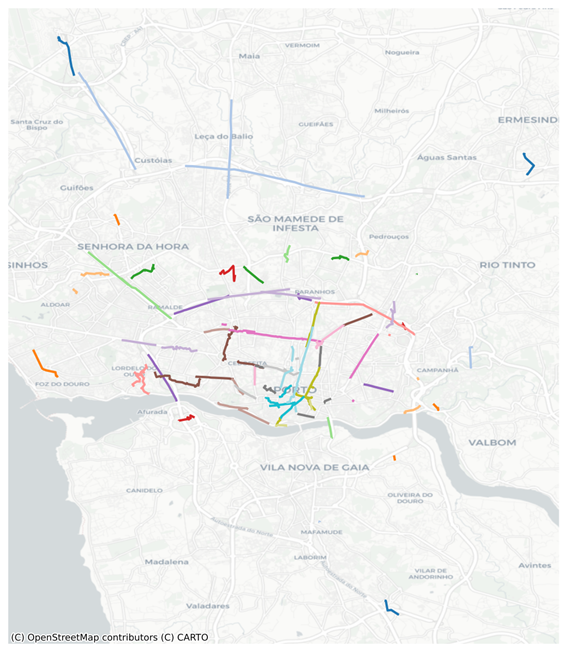
\includegraphics[width=0.5\textwidth]{img/r_tray_HDBSCAN.png}
    \caption{Representación de trayectorias.}
    \label{fig:trayectorias_HDBSCAN}
\end{figure}

\FloatBarrier

\item \textbf{Agglomerative Clustering}:  
Este algoritmo requería definir previamente el número de clusters. En este caso, se utilizaron los 2654 segmentos generados, sin descartar ninguno, ya que no clasifica datos como "basura". Sin embargo, esta característica provoca que los clusters no se centren en las zonas más densas, lo que resulta en representaciones de trayectorias más erráticas.

\begin{figure}[h!]
    \centering
    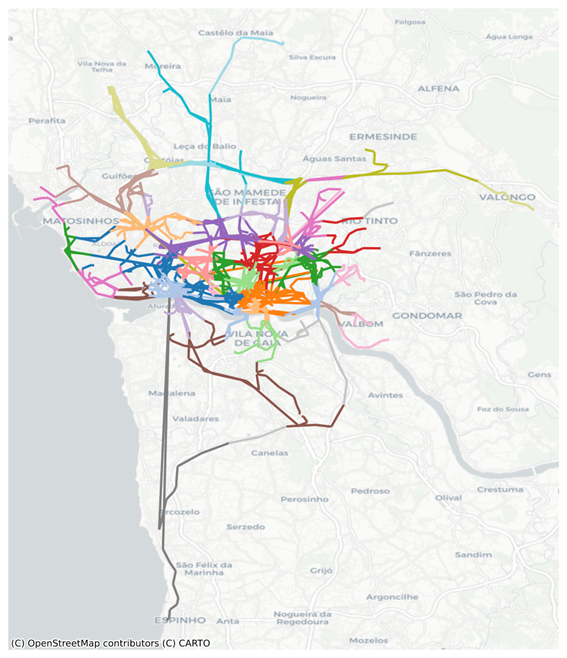
\includegraphics[width=0.5\textwidth]{img/clusters_Aggl.png}
    \caption{Representación de clusters.}
    \label{fig:clusters_Agglomerative}
\end{figure}

\begin{figure}[h!]
    \centering
    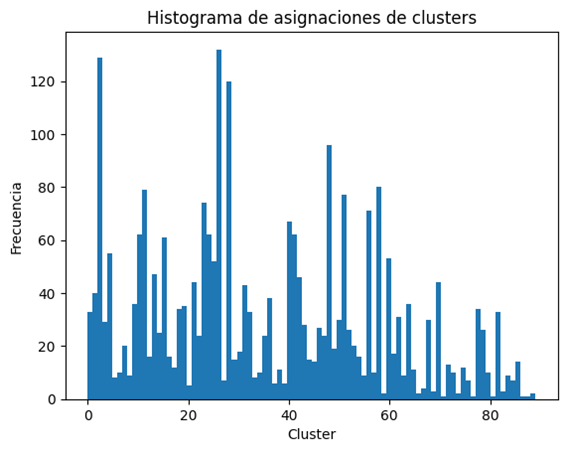
\includegraphics[width=0.5\textwidth]{img/histograma_Aggl.png}
    \caption{Segmentos por cada cluster.}
    \label{fig:histograma_Agglomerative}
\end{figure}

\begin{figure}[h!]
    \centering
    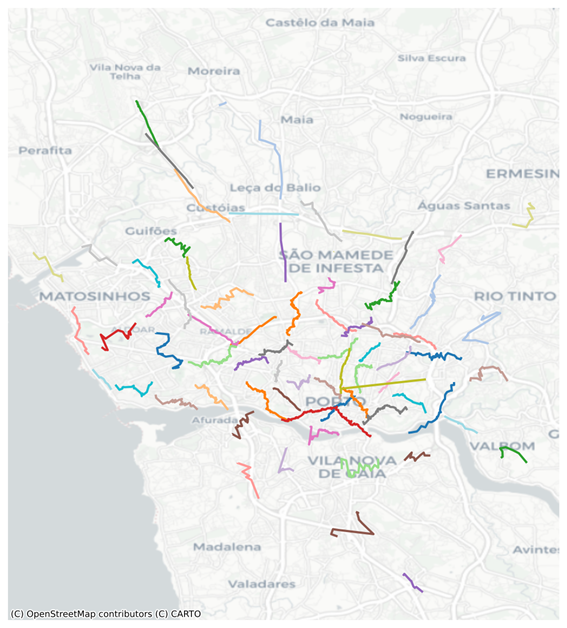
\includegraphics[width=0.5\textwidth]{img/r_tray_Aggl.png}
    \caption{Representación de trayectorias.}
    \label{fig:trayectorias_Agglomerative}
\end{figure}

\FloatBarrier

\item \textbf{Spectral Clustering}:  
Al igual que el algoritmo anterior, no descarta datos. Aunque se generaron los mismos 2654 segmentos y clusters que en Agglomerative Clustering, los resultados finales fueron diferentes, con una distribución menos centralizada.

\begin{figure}[h!]
    \centering
    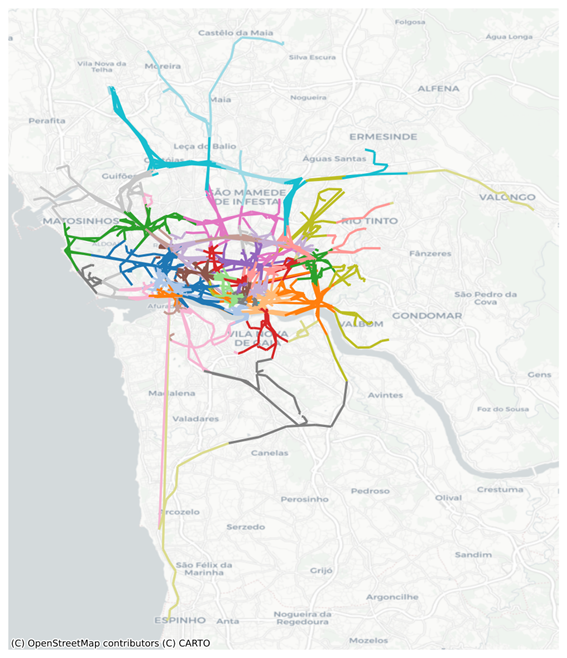
\includegraphics[width=0.5\textwidth]{img/clusters_Spect.png}
    \caption{Representación de clusters.}
    \label{fig:clusters_Spectral}
\end{figure}

\begin{figure}[h!]
    \centering
    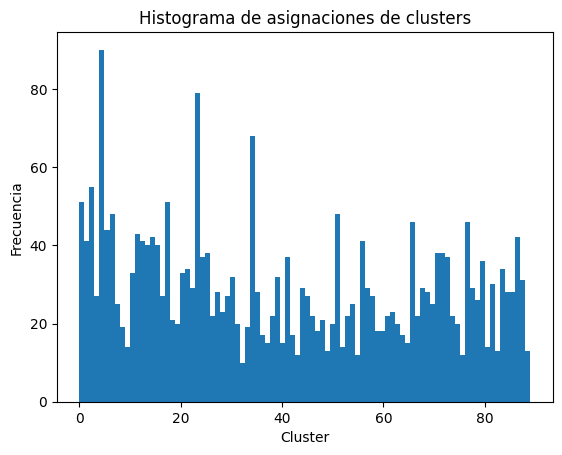
\includegraphics[width=0.5\textwidth]{img/histograma_Spect.png}
    \caption{Segmentos por cada cluster.}
    \label{fig:histograma_Spectral}
\end{figure}

\begin{figure}[h!]
    \centering
    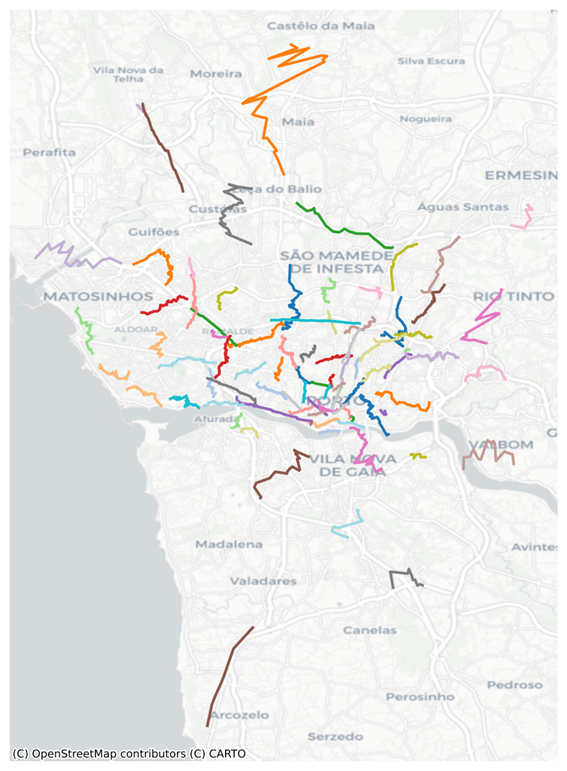
\includegraphics[width=0.5\textwidth]{img/r_tray_Spect.png}
    \caption{Representación de trayectorias.}
    \label{fig:trayectorias_Spectral}
\end{figure}

\FloatBarrier

\end{enumerate}

\subsection{Conclusión}

La comparativa de algoritmos de \textit{clustering} mostró diferencias significativas en los resultados obtenidos, claramente visibles en las imágenes de los clusters generados. Aunque se utilizó un conjunto de datos con 200 filas, aumentar la cantidad de datos podría mejorar la robustez de los resultados y proporcionar patrones más generalizables. En esta evaluación, \textbf{Spectral Clustering} y \textbf{Agglomerative Clustering} carecieron de configuraciones de parámetros que generaran clusters bien definidos, lo que resultó en trayectorias dispersas y difíciles de analizar. Por el contrario, \textbf{OPTICS} y \textbf{HDBSCAN} produjeron resultados más consistentes, siendo HDBSCAN el que clasificó un menor porcentaje de segmentos como "basura".

\textbf{DBSCAN} mostró una tendencia hacia rutas centralizadas, aunque con una tasa alta de segmentos descartados. Esto sugiere que DBSCAN podría ser más efectivo para identificar trayectorias centrales claras, aunque a costa de una menor utilización de datos. La elección del algoritmo más adecuado dependerá del contexto específico y de la importancia relativa de la densidad frente a la centralización de las rutas.

\begin{table}[ht]
\centering
\begin{tabular}{|l|c|c|c|}
\hline
\textbf{Algoritmo} & \textbf{Segmentos} & \textbf{Segmentos 'basura'} & \textbf{Clusters}  \\
\hline
OPTICS & 2161 & 62.66\% & 106 \\
DBSCAN & 2654 & 90.09\% & 37 \\
HDBSCAN & 2161 & 53.54\% & 96 \\
Spectral Clustering & 2654 & 0\% & 90 \\
Agglomerative Clustering & 2654 & 0\% & 90 \\
\hline
\end{tabular}
\caption{Resumen de resultados de los algoritmos de clustering}
\label{tabla:comparacion_algoritmos}
\end{table}



\section{Pruebas funcionales}

Para demostrar la utilidad del algoritmo y la aplicación creados, se propuso realizar múltiples pruebas con diferentes conjuntos de datos, tamaños y configuraciones aplicados a los algoritmos de clustering.

\subsection{Conjuntos de datos}

Durante el desarrollo del proyecto, se utilizó en prácticamente todo el conjunto de datos de Trayectorias Taxis \cite{trayectorias_taxis}. Para esta comprobación final, esto no era suficiente. Usar solo este conjunto de datos limitaría el proyecto a un análisis específico. Por lo tanto, se buscó encontrar múltiples conjuntos de datos.

Aunque existen multitud de conjuntos de datos con coordenadas GPS que pueden servir la mayoría de ellos no se encuentran en un formato preparado para correr el TRACLUS. Normalmente los conjuntos suelen separar las coordenadas en puntos lo cual no es valido ya que el TRACLUS, este necesita de trayectorias por tanto hay que juntar los datos de forma lógica con un formato valido. 

El primer conjunto con esa estructura adaptada fue Geolife \cite{geolife_trajectories}. Este estudio organiza los datos en carpetas, una por cada sujeto al que se le registraron ubicaciones durante un periodo de tiempo. Dentro de cada carpeta se encontraban varios archivos \texttt{.plt} que contenían información sobre la latitud, longitud, hora y fecha de las mediciones. 

Para organizar los datos de forma lógica para el algoritmo TRACLUS, no era viable crear una fila por cada archivo \texttt{.plt}, ya que algunos contenían más de 1000 mediciones. Por lo tanto, se decidió agrupar las mediciones por hora. Todas las mediciones tomadas dentro de la misma hora se combinaron en una única fila de un archivo Excel.

Se creó una función para automatizar este proceso por carpeta, lo que permitió realizar pruebas fácilmente en diferentes sujetos. Para analizar los resultados, se utilizó un archivo Excel generado con todos los datos encontrados en la carpeta del sujeto \texttt{000}.

Otro conjunto de datos probado fue uno de MoveBank \cite{movebank}, una plataforma que contiene miles de trayectorias de animales. Debido a la inmensidad de opciones disponibles, se seleccionó de forma semi-aleatoria el conjunto de datos titulado \textit{"Hammer-headed fruit bats (Hypsignathus monstrosus) in the Republic of Congo"}. Este conjunto incluía datos de múltiples murciélagos de la fruta registrados en diferentes días. 

Tras analizar el número de mediciones por hora, se decidió dividir las trayectorias por murciélago y día, creando un conjunto de datos con filas más reducidas en comparación al anterior. Aun así, estas filas eran considerablemente más grandes que las del conjunto de Trayectorias Taxis, lo cual incrementó significativamente el tiempo de procesamiento por cada fila analizada.

Ademas de estos tres se hicieron pruebas con otros como Citi Bikes \cite{citybike} o Foursquare-NY \cite{foursquare} pero los resultado no fueron visualmente atractivos para un buen analisis y muestra.

\subsection{Criterios para las pruebas:}

\begin{enumerate}
    \item \textbf{Límite de tiempo:} Cada prueba debe durar un máximo de dos horas, considerando tanto el tiempo de ejecución como el de representación de los datos. Este límite puede variar según el tamaño del conjunto de datos y el número de coordenadas procesadas.
    \item \textbf{Selección de parámetros:} No se probarán todas las combinaciones posibles. Se seleccionarán aquellas configuraciones que se consideren más relevantes y que puedan producir cambios significativos en los resultados.
    \item \textbf{Parámetros predeterminados:} En las pruebas que uno de los elementos se cambie el resto de ellos permanecerán con los siguientes valores: 
    
    \begin{itemize}
    		\item \textbf{Metric:} \texttt{euclidean}
    		\item \textbf{Algorithm:} \texttt{auto}
    		\item \textbf{Min\_samples:} 5
   		\item \textbf{Max\_eps:} 1
    		\item \textbf{Eps:} 0.1
    		\item \textbf{Linkage:} \texttt{ward}
    		\item \textbf{Affinity:} \texttt{nearest\_neighbors}
    		\item \textbf{Assign\_labels:} \texttt{kmeans}
    		\item \textbf{n\_clusters:} 7
	\end{itemize}

\end{enumerate}

\subsection{Resultados}

\subsubsection{OPTICS, DBSCAN y HDBSCAN}

En las pruebas iniciales, se observó que, debido a las características de los datos seleccionados, los algoritmos OPTICS y HDBSCAN tendían a comportarse de manera similar, con la principal diferencia siendo el parámetro \texttt{Max\_eps}, esta se calcula internamente en HDBSCAN por lo que dependiendo de la cantidad de datos esta cambiara. Por otro lado, DBSCAN también podría reproducir resultados similares bajo configuraciones específicas del parámetro \texttt{eps}. 

Para comprender cómo los parámetros afectan el rendimiento de cada algoritmo, se realizaron pruebas aislando cada parámetro. Es decir, al modificar un parámetro, los demás permanecieron en sus valores predeterminados.

\paragraph{Métricas (\texttt{metric})}

Las métricas utilizadas para calcular las distancias entre puntos demostraron tener un impacto significativo en los resultados. Los hallazgos principales fueron los siguientes:

- \textbf{Métricas no funcionales}: Algunas métricas, como \texttt{l1} y \texttt{cosine}, no pudieron procesar correctamente los datos seleccionados, lo que resultó en errores o en agrupaciones inadecuadas, sin embargo con otras cantidades u otros parámetros estas si que dieron resultado.

- \textbf{Manhattan}: Esta métrica tendió a considerar todos los puntos como parte de un único clúster grande, resultando en una agrupación poco informativa. En el caso de las trayectorias, esto significó un único grupo, lo que limitó el análisis.

\begin{figure}[h!]
    \centering
    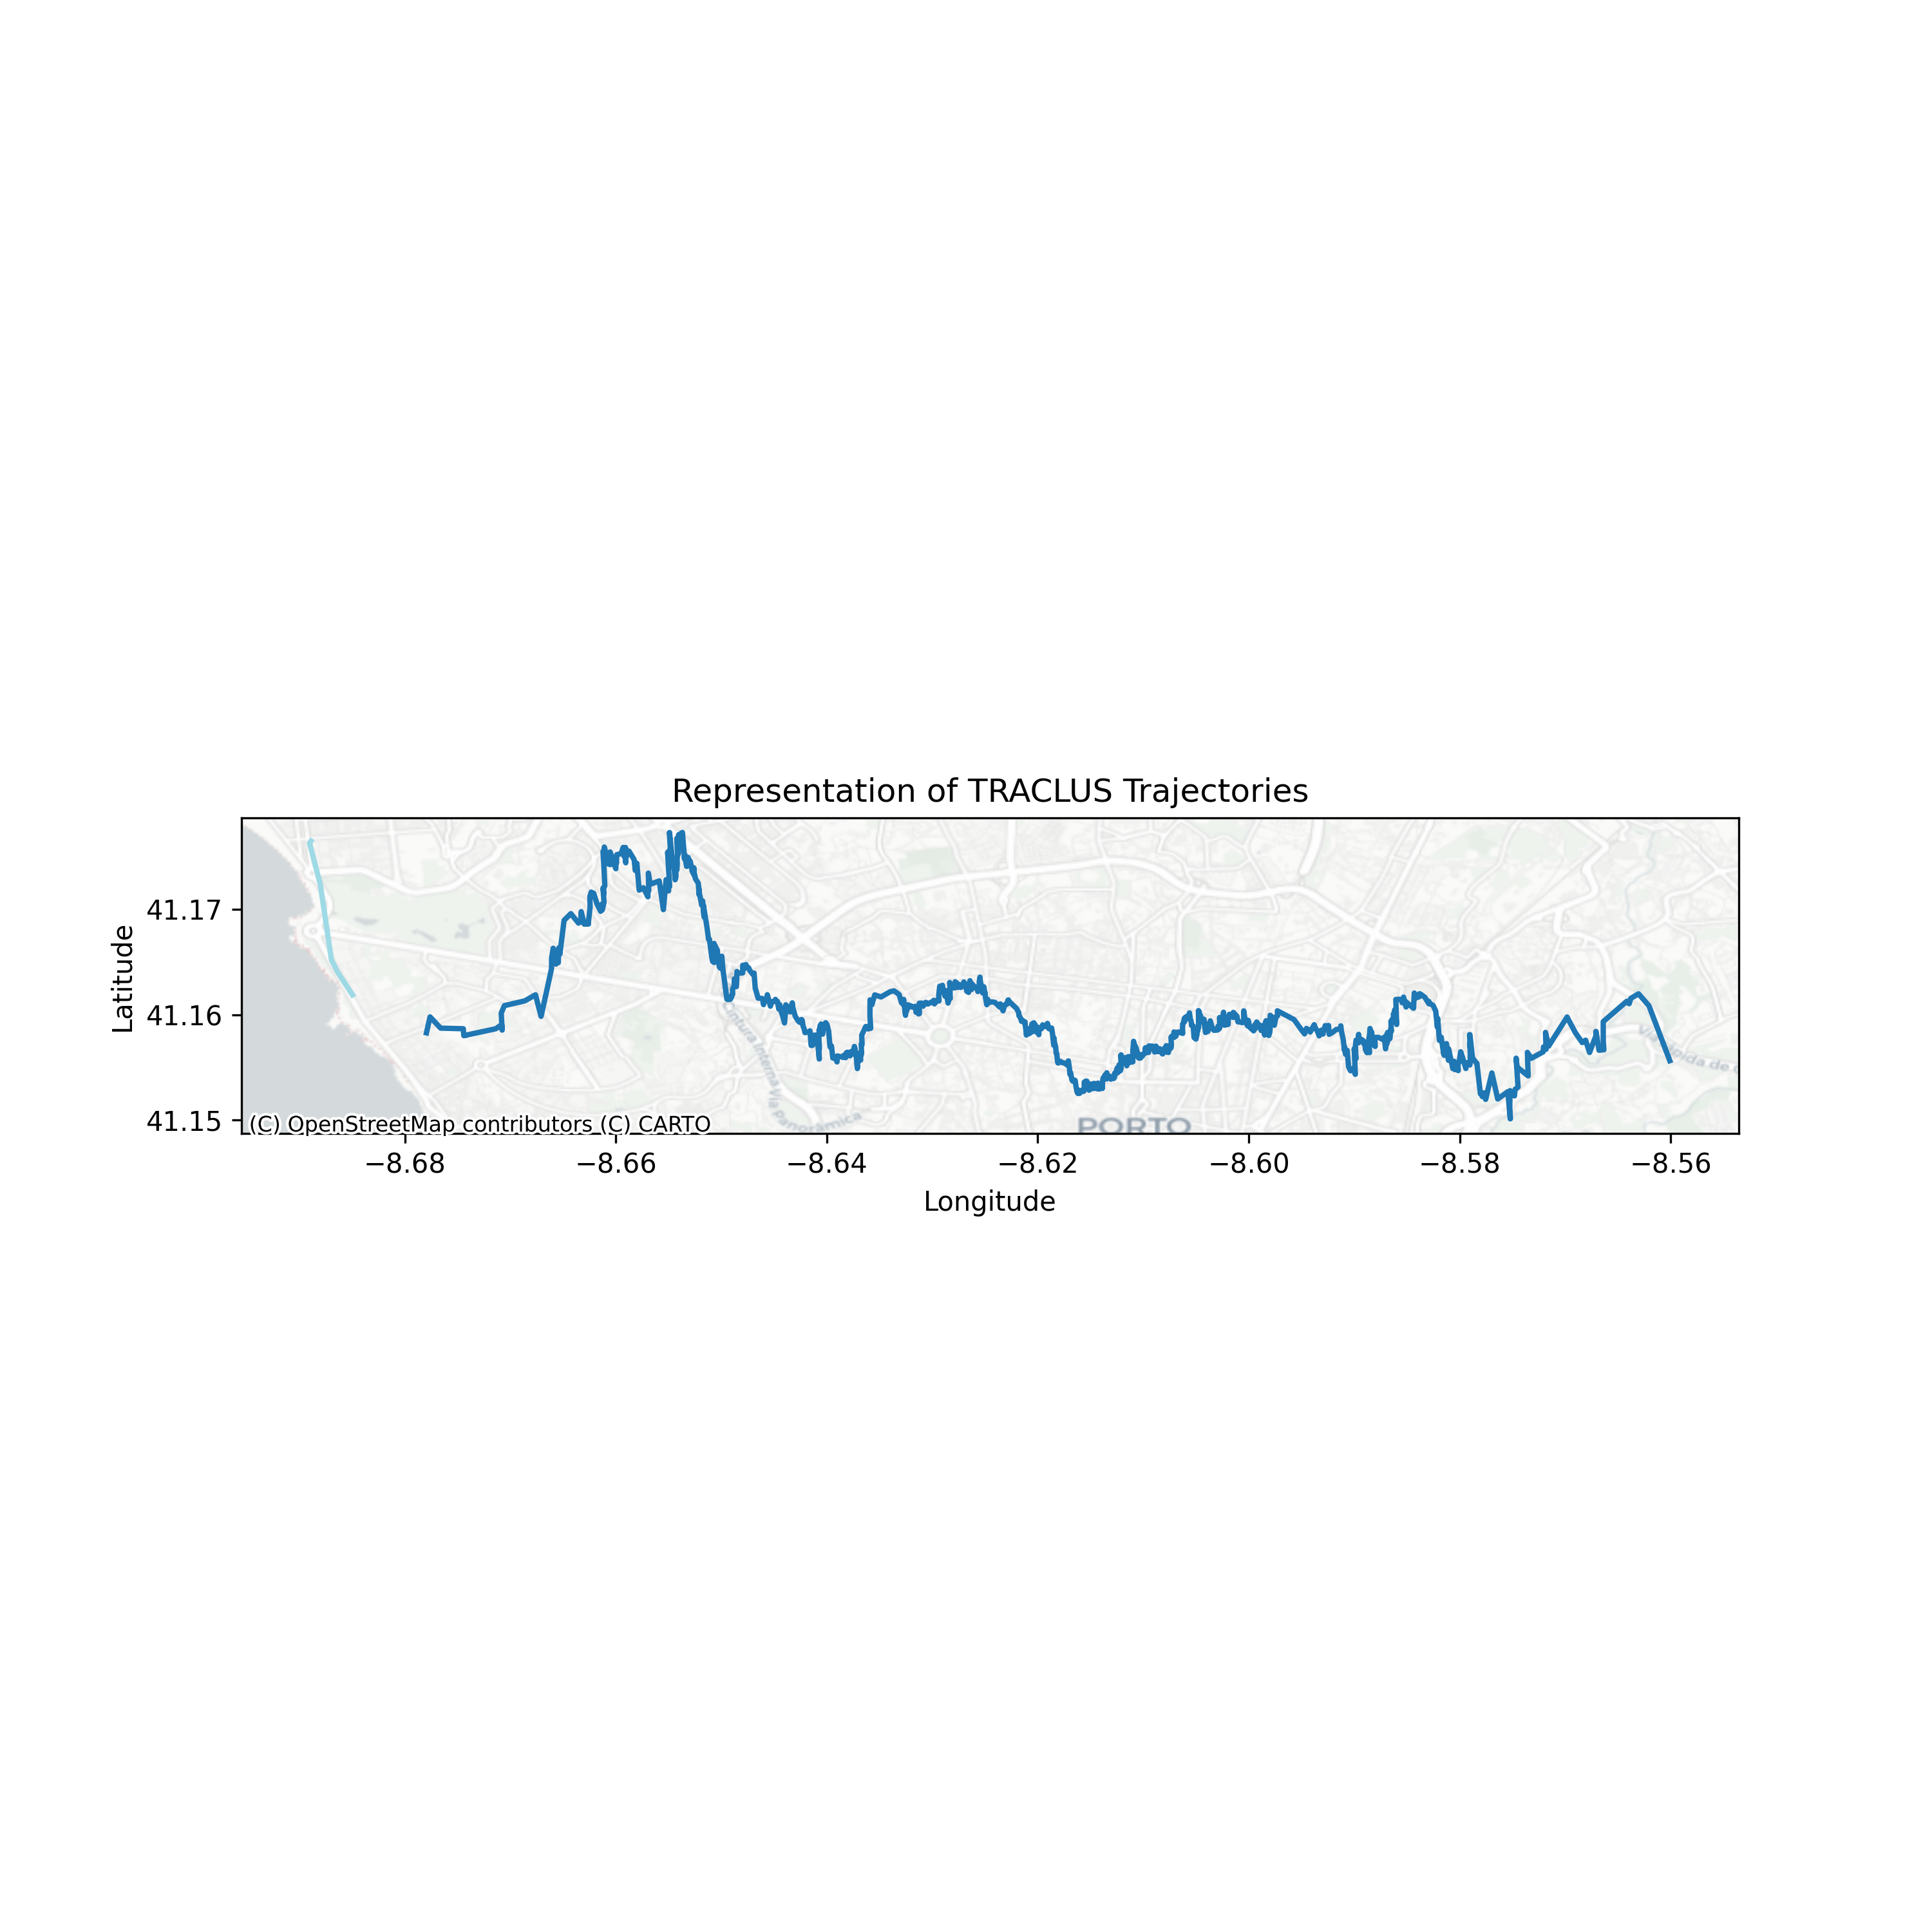
\includegraphics[width=0.8\textwidth]{img/Taxis/map_optics_manhatan.png}
    \caption{Resultados con la métrica Manhattan en OPTICS y HDBSCAN.}
    \label{fig:manhattan}
\end{figure}

\FloatBarrier

- \textbf{Euclidean y L2}: Ambas métricas ofrecieron resultados idénticos, creando agrupaciones claras y comprensibles. Estas métricas son particularmente adecuadas para este tipo de datos.

\begin{figure}[h!]
    \centering
    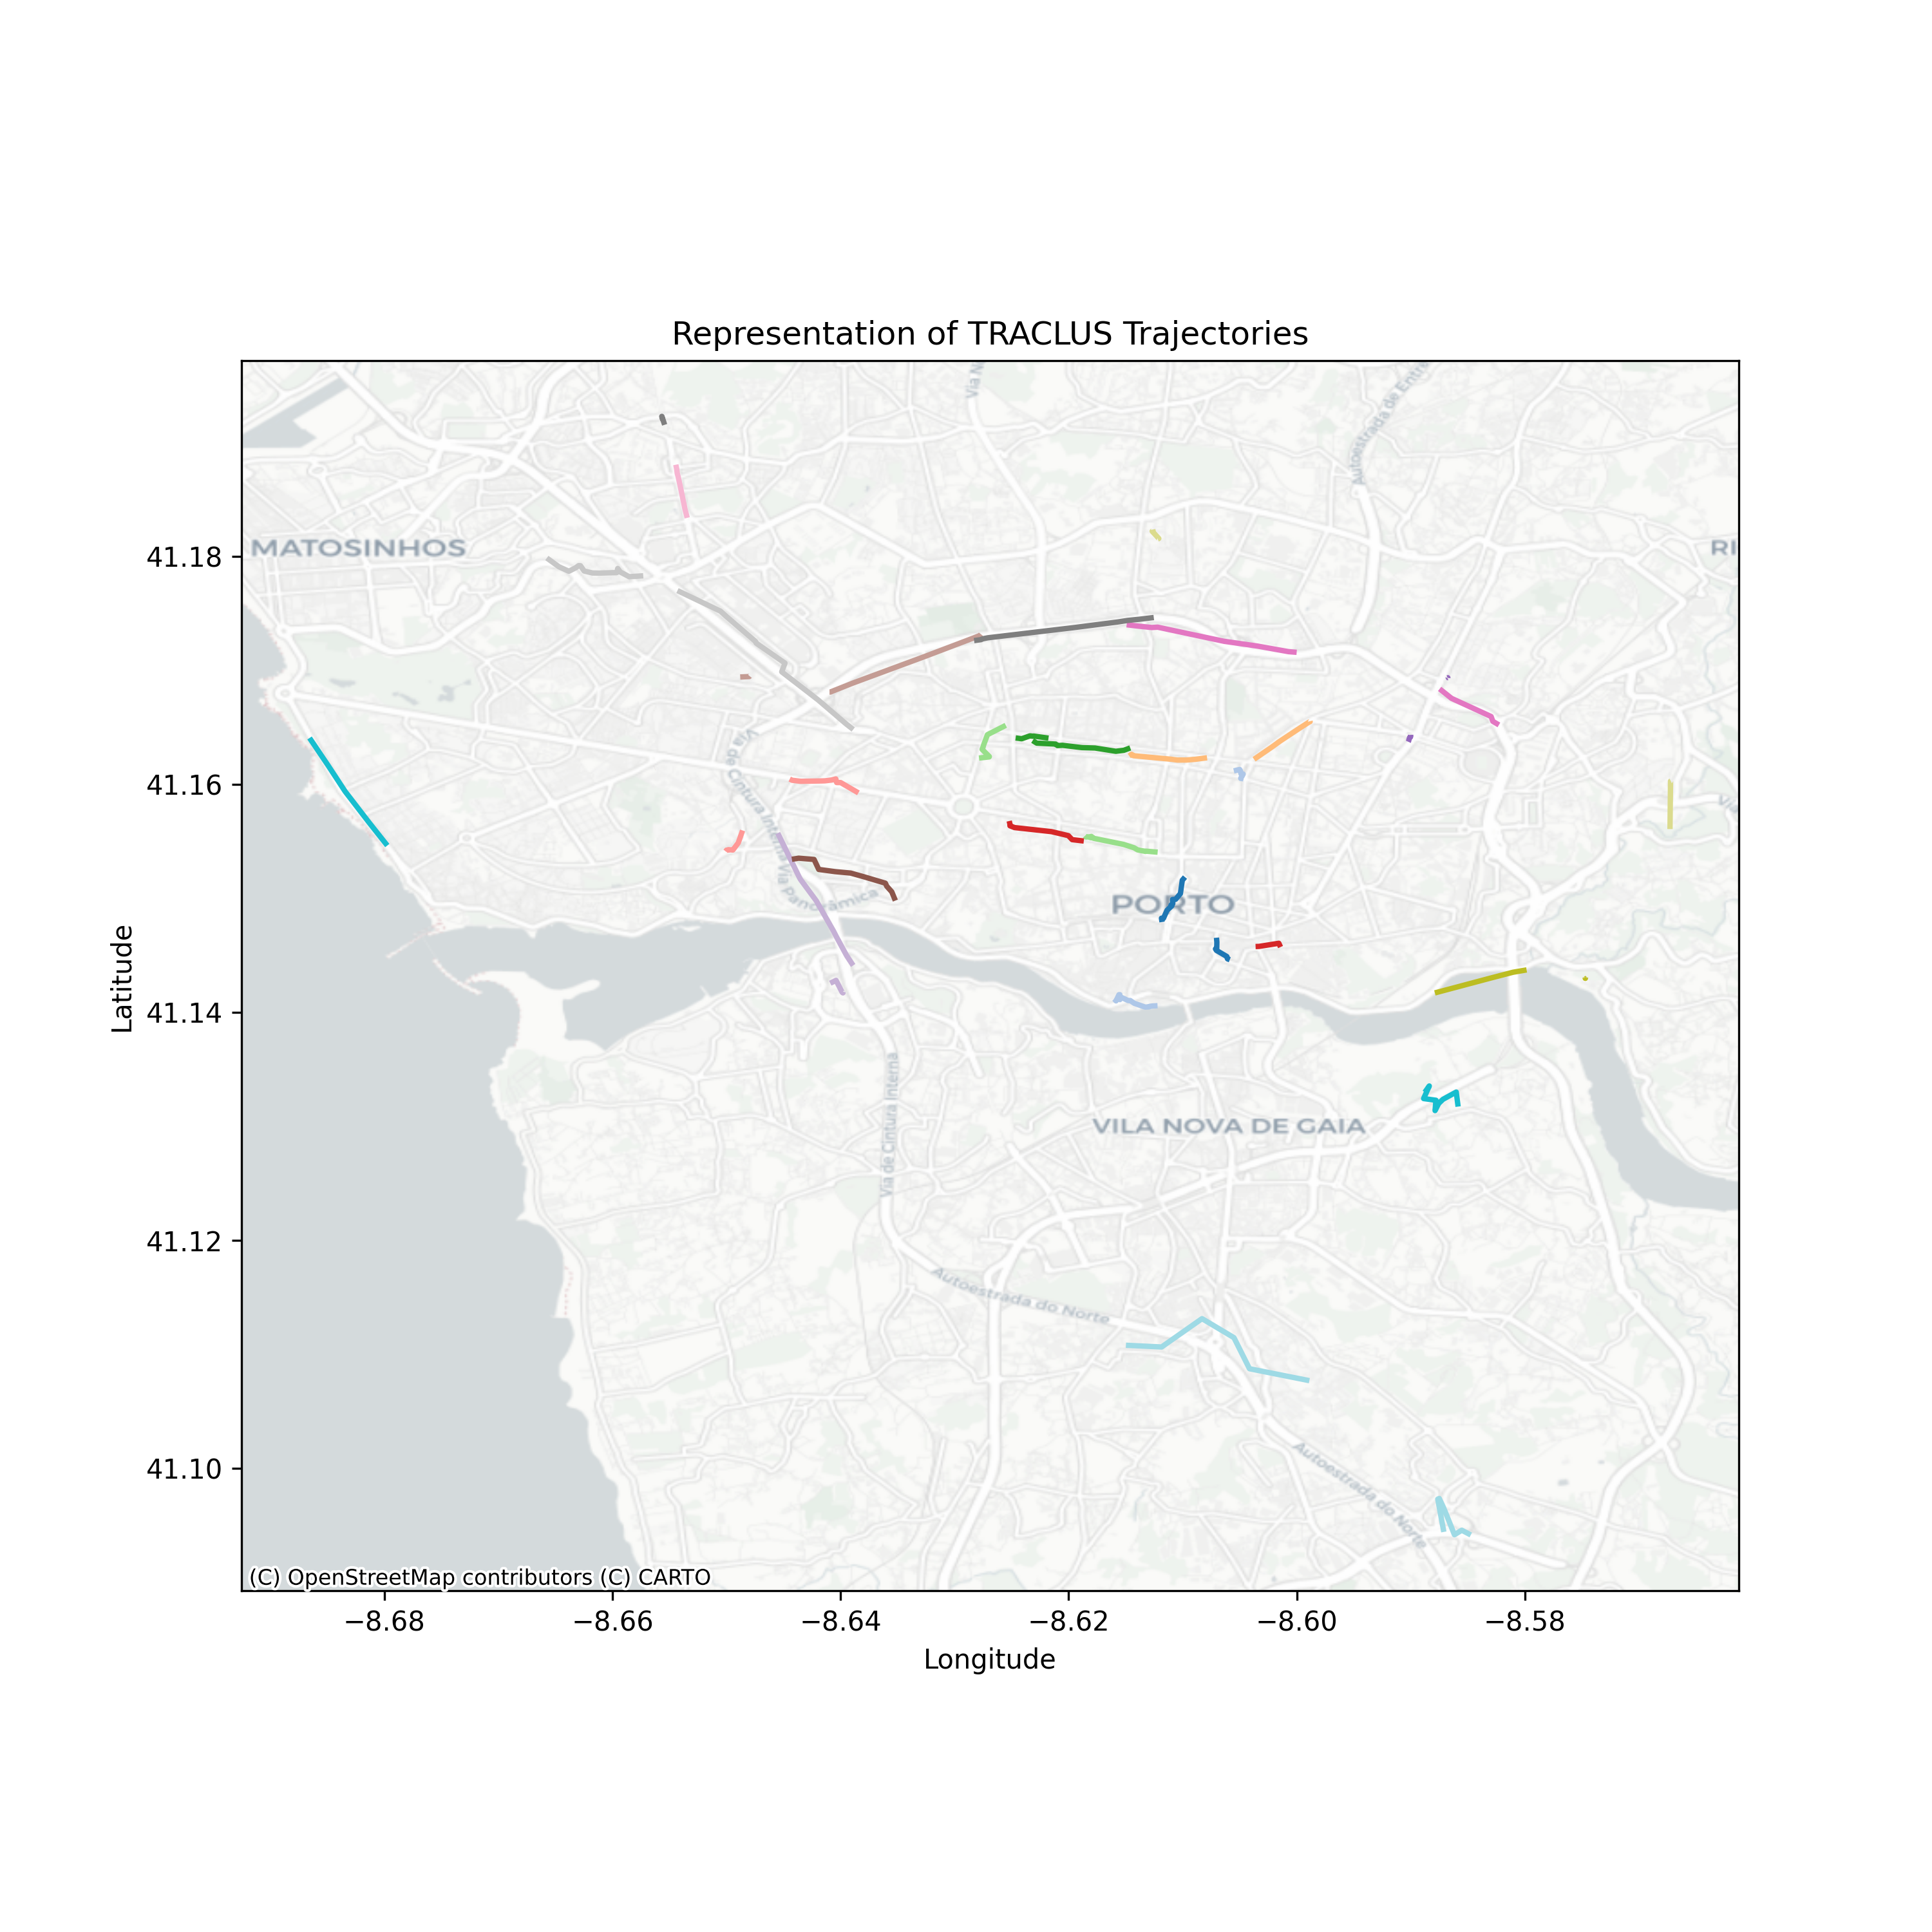
\includegraphics[width=0.8\textwidth]{img/Taxis/map_optics_l2.png}
    \caption{Resultados con las métricas Euclidean y L2 en OPTICS y HDBSCAN.}
    \label{fig:euclidean}
\end{figure}

\FloatBarrier

- \textbf{Cityblock}: Aunque mostró similitudes con las métricas anteriores, los clústeres resultantes eran menos definidos y algo más dispersos, lo que afectó la precisión de las trayectorias.

\begin{figure}[h!]
    \centering
    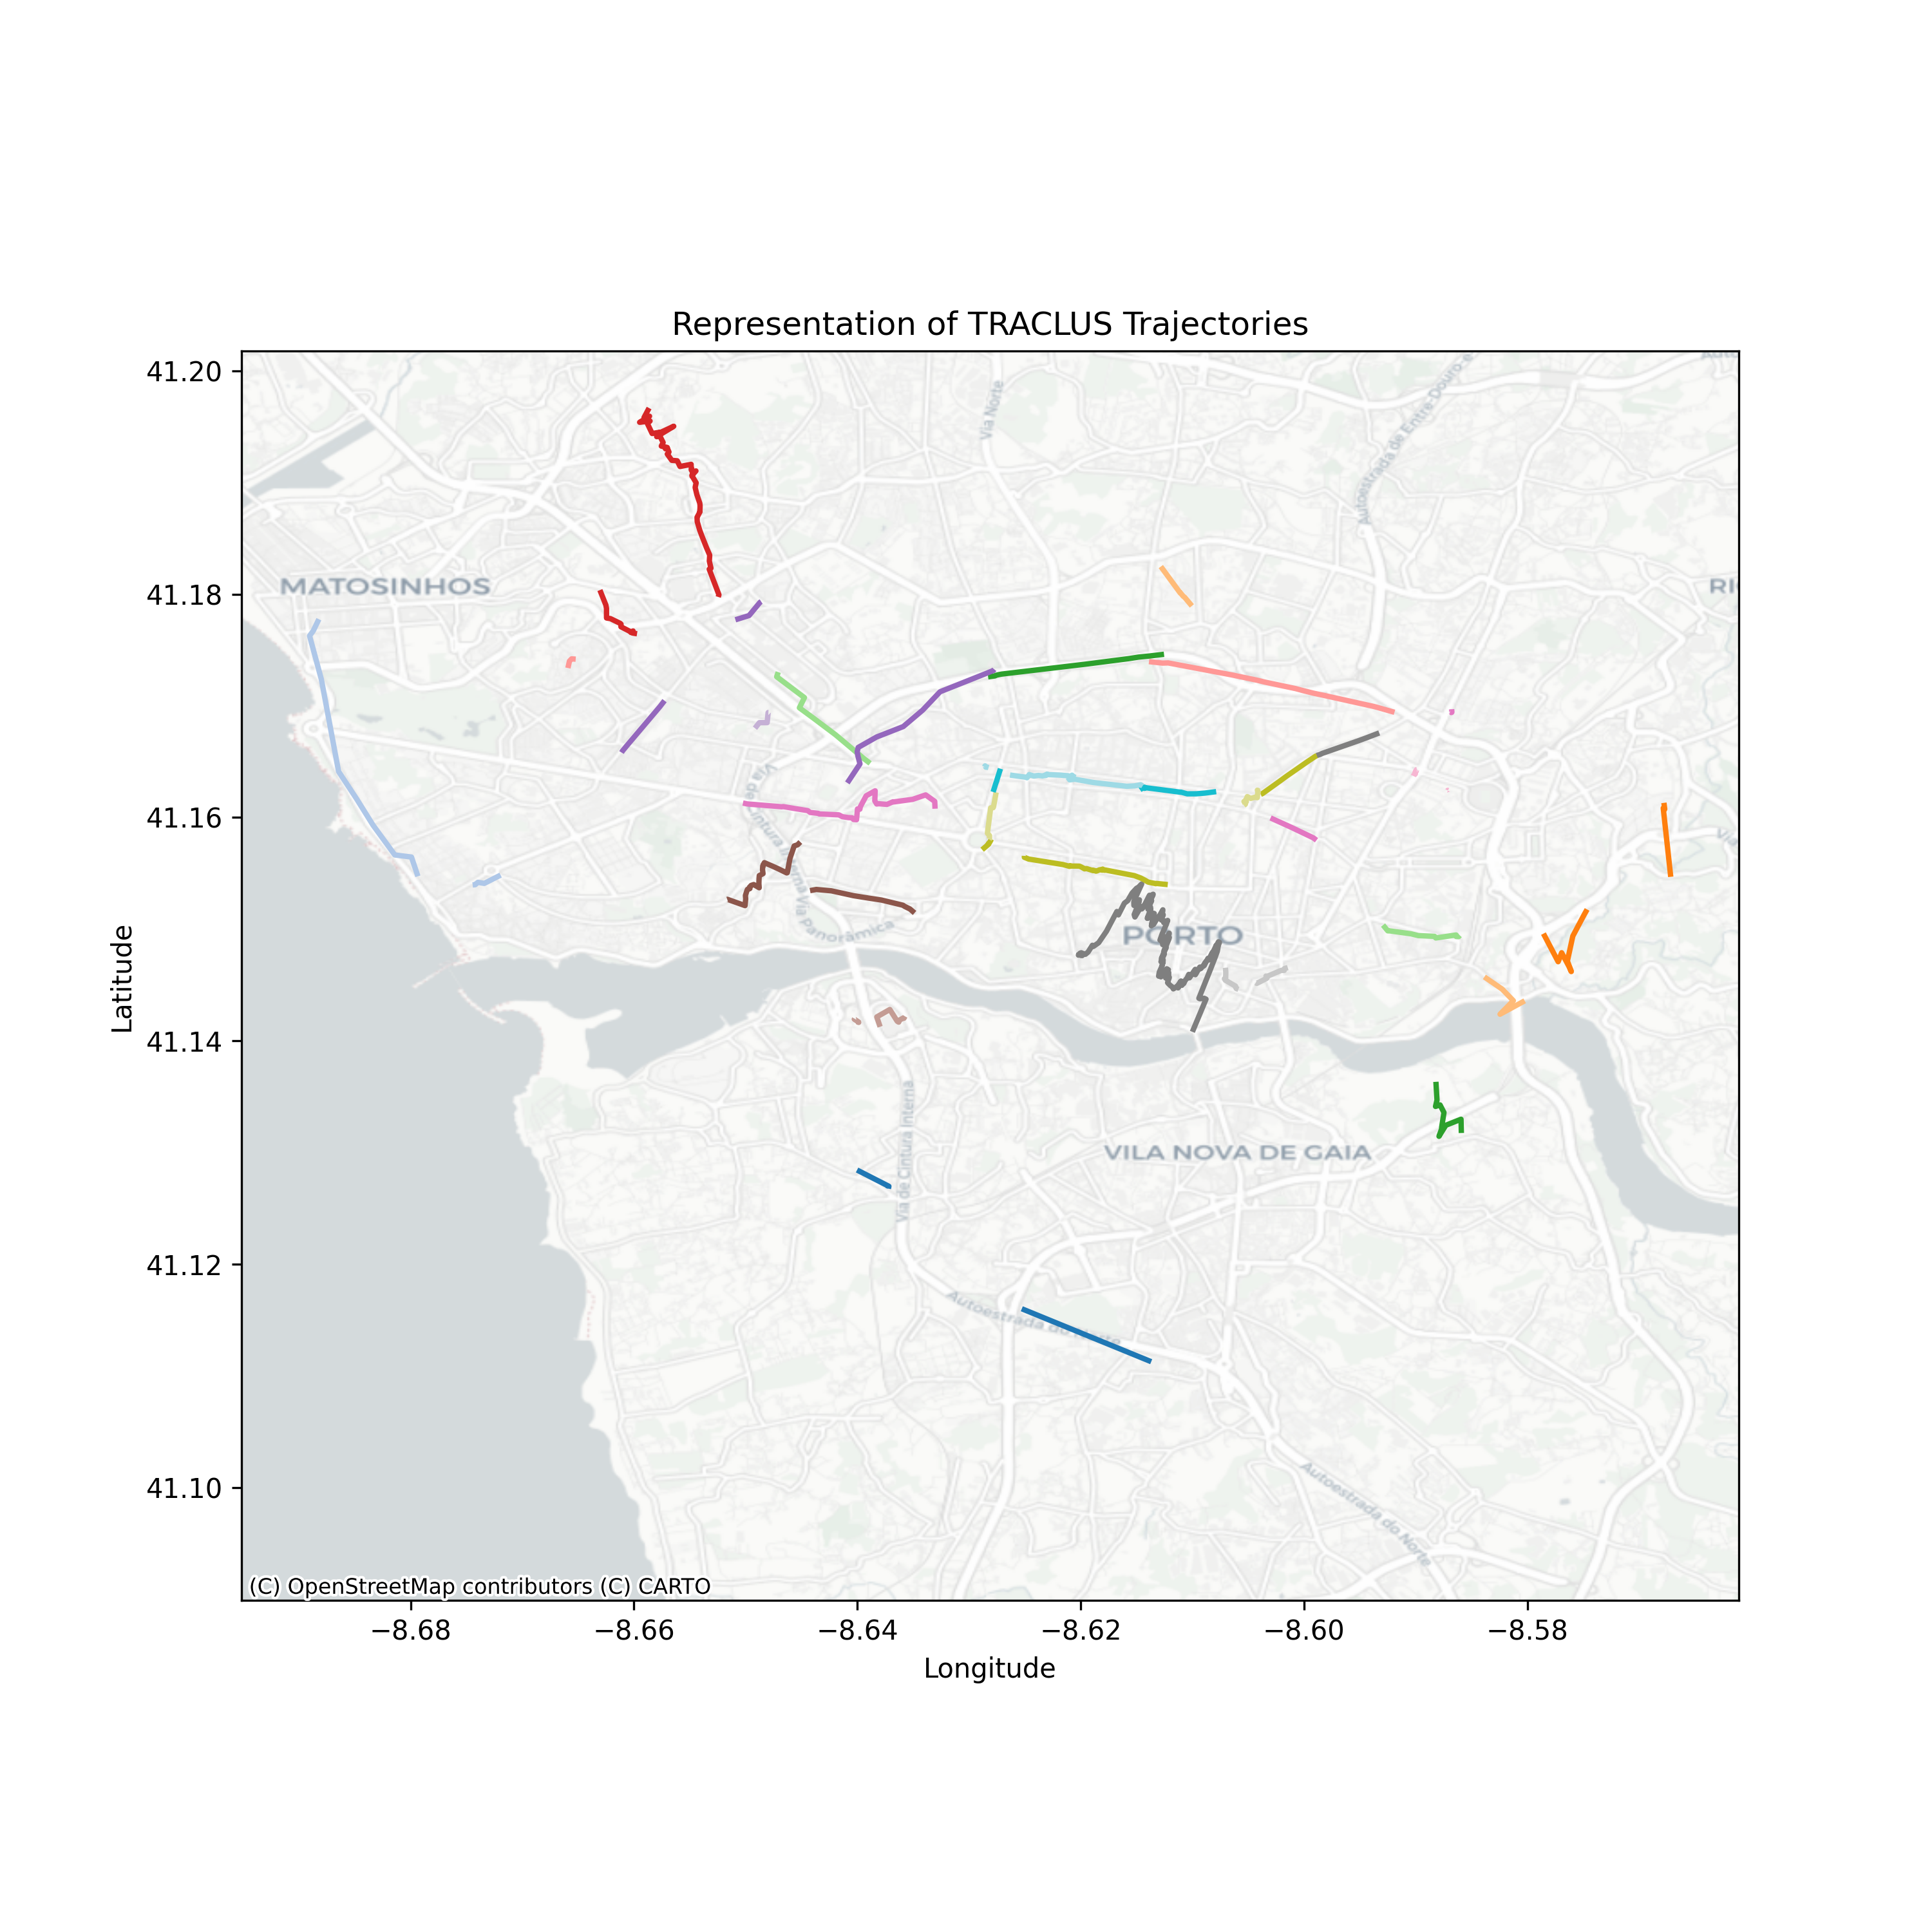
\includegraphics[width=0.8\textwidth]{img/Taxis/map_optics_city.png}
    \caption{Resultados con la métrica Cityblock en OPTICS y HDBSCAN.}
    \label{fig:cityblock}
\end{figure}

\FloatBarrier

En general, se determinó que el uso de métricas como Euclidean o L2 es más recomendable, mientras que Manhattan y otras métricas no lineales presentaron limitaciones significativas en este conjunto de datos. Sin embargo, esta conclusión no se pude aplicar en cambios de todos los parámetros.


\paragraph{Algoritmo (\texttt{algorithm})}

El parámetro \texttt{algorithm} define la estrategia interna utilizada por el algoritmo para calcular los clústeres. Los resultados variaron dependiendo del conjunto de datos empleado:

-\textbf{Trayectorias Taxis}:

A diferencia de las metricas que si se comportaban de la misma forma en los tres algoritmos, el parametro algoritmo variaba en gran mediada, para empezar, OPTICS no recibia cambios dando igual cual de ellas se probara.

\begin{figure}[h!]
    \centering
    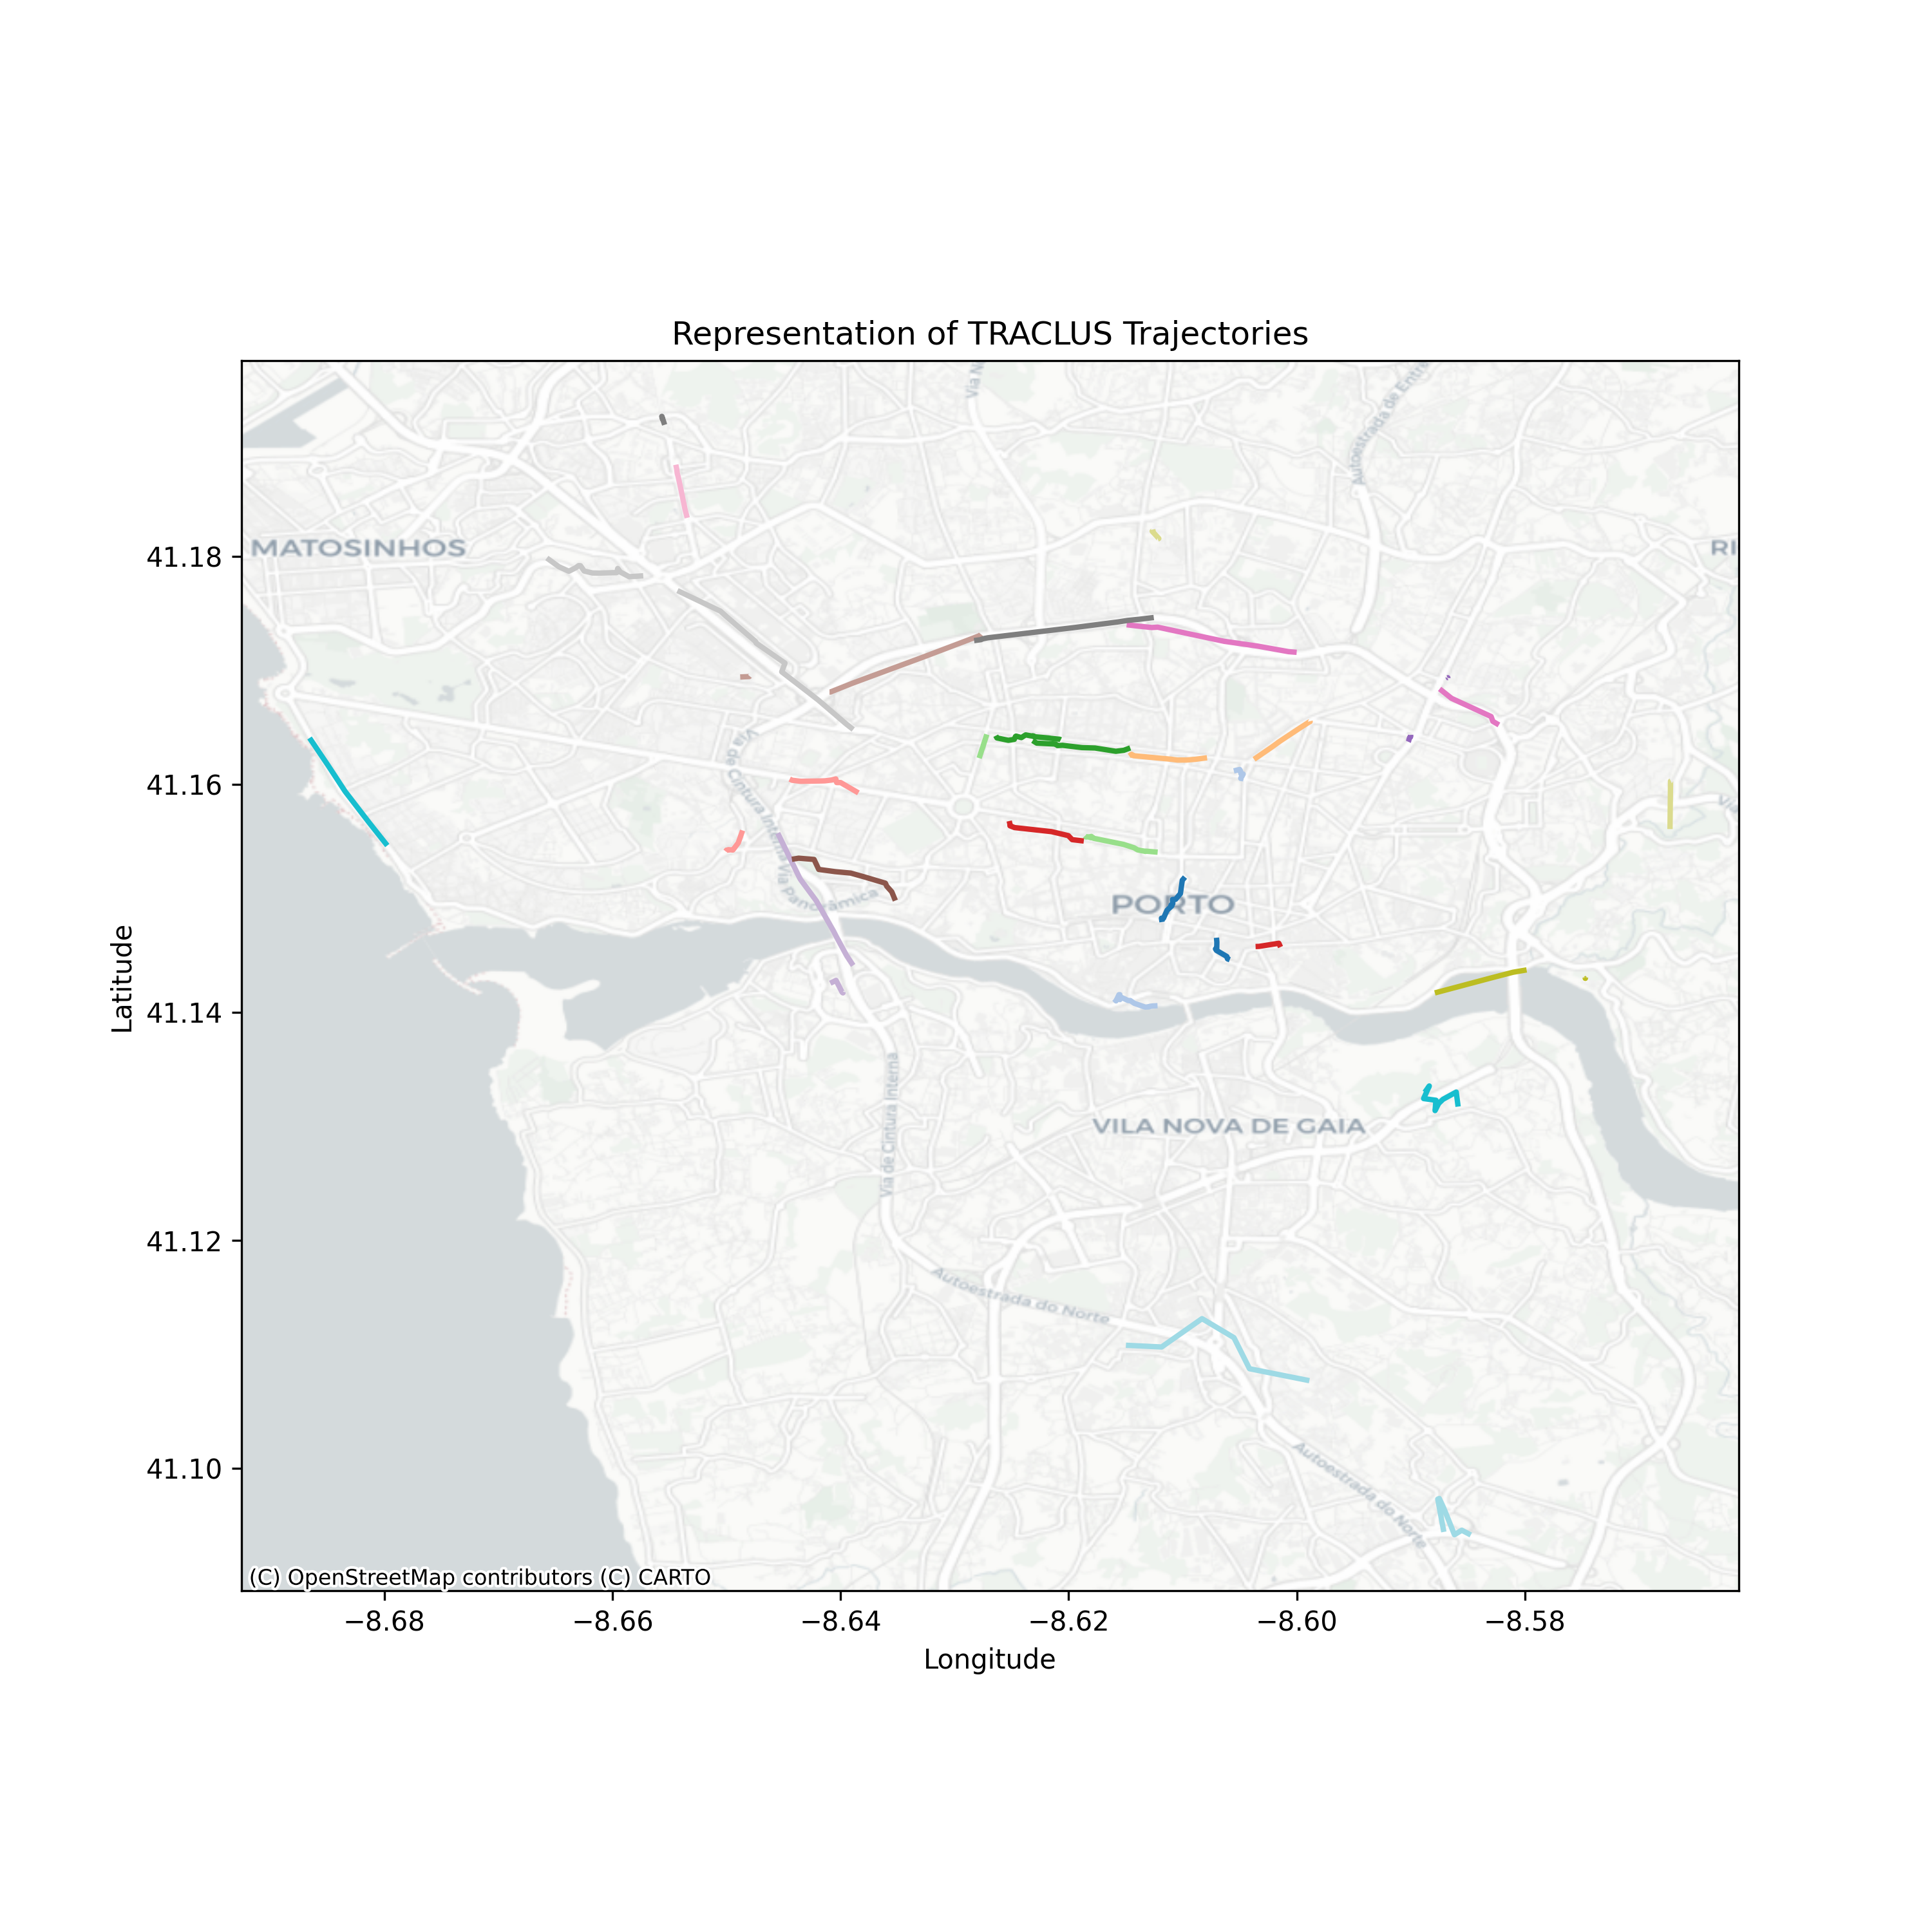
\includegraphics[width=0.5\textwidth]{img/Taxis/map_optics_auto.png}
    \caption{Resultados con todos los algoritmos en OPTICS.}
    \label{fig:taxis_algorith_optics}
\end{figure}

\FloatBarrier

De la misma forma DBSCAN y HDBSCAN, ambas tienen los mismos resultados en cada algoritmo, aun cambiando el resto de datos, los diferentes algoritmos no parecían variar el resultado.

\begin{figure}[h!]
    \centering
    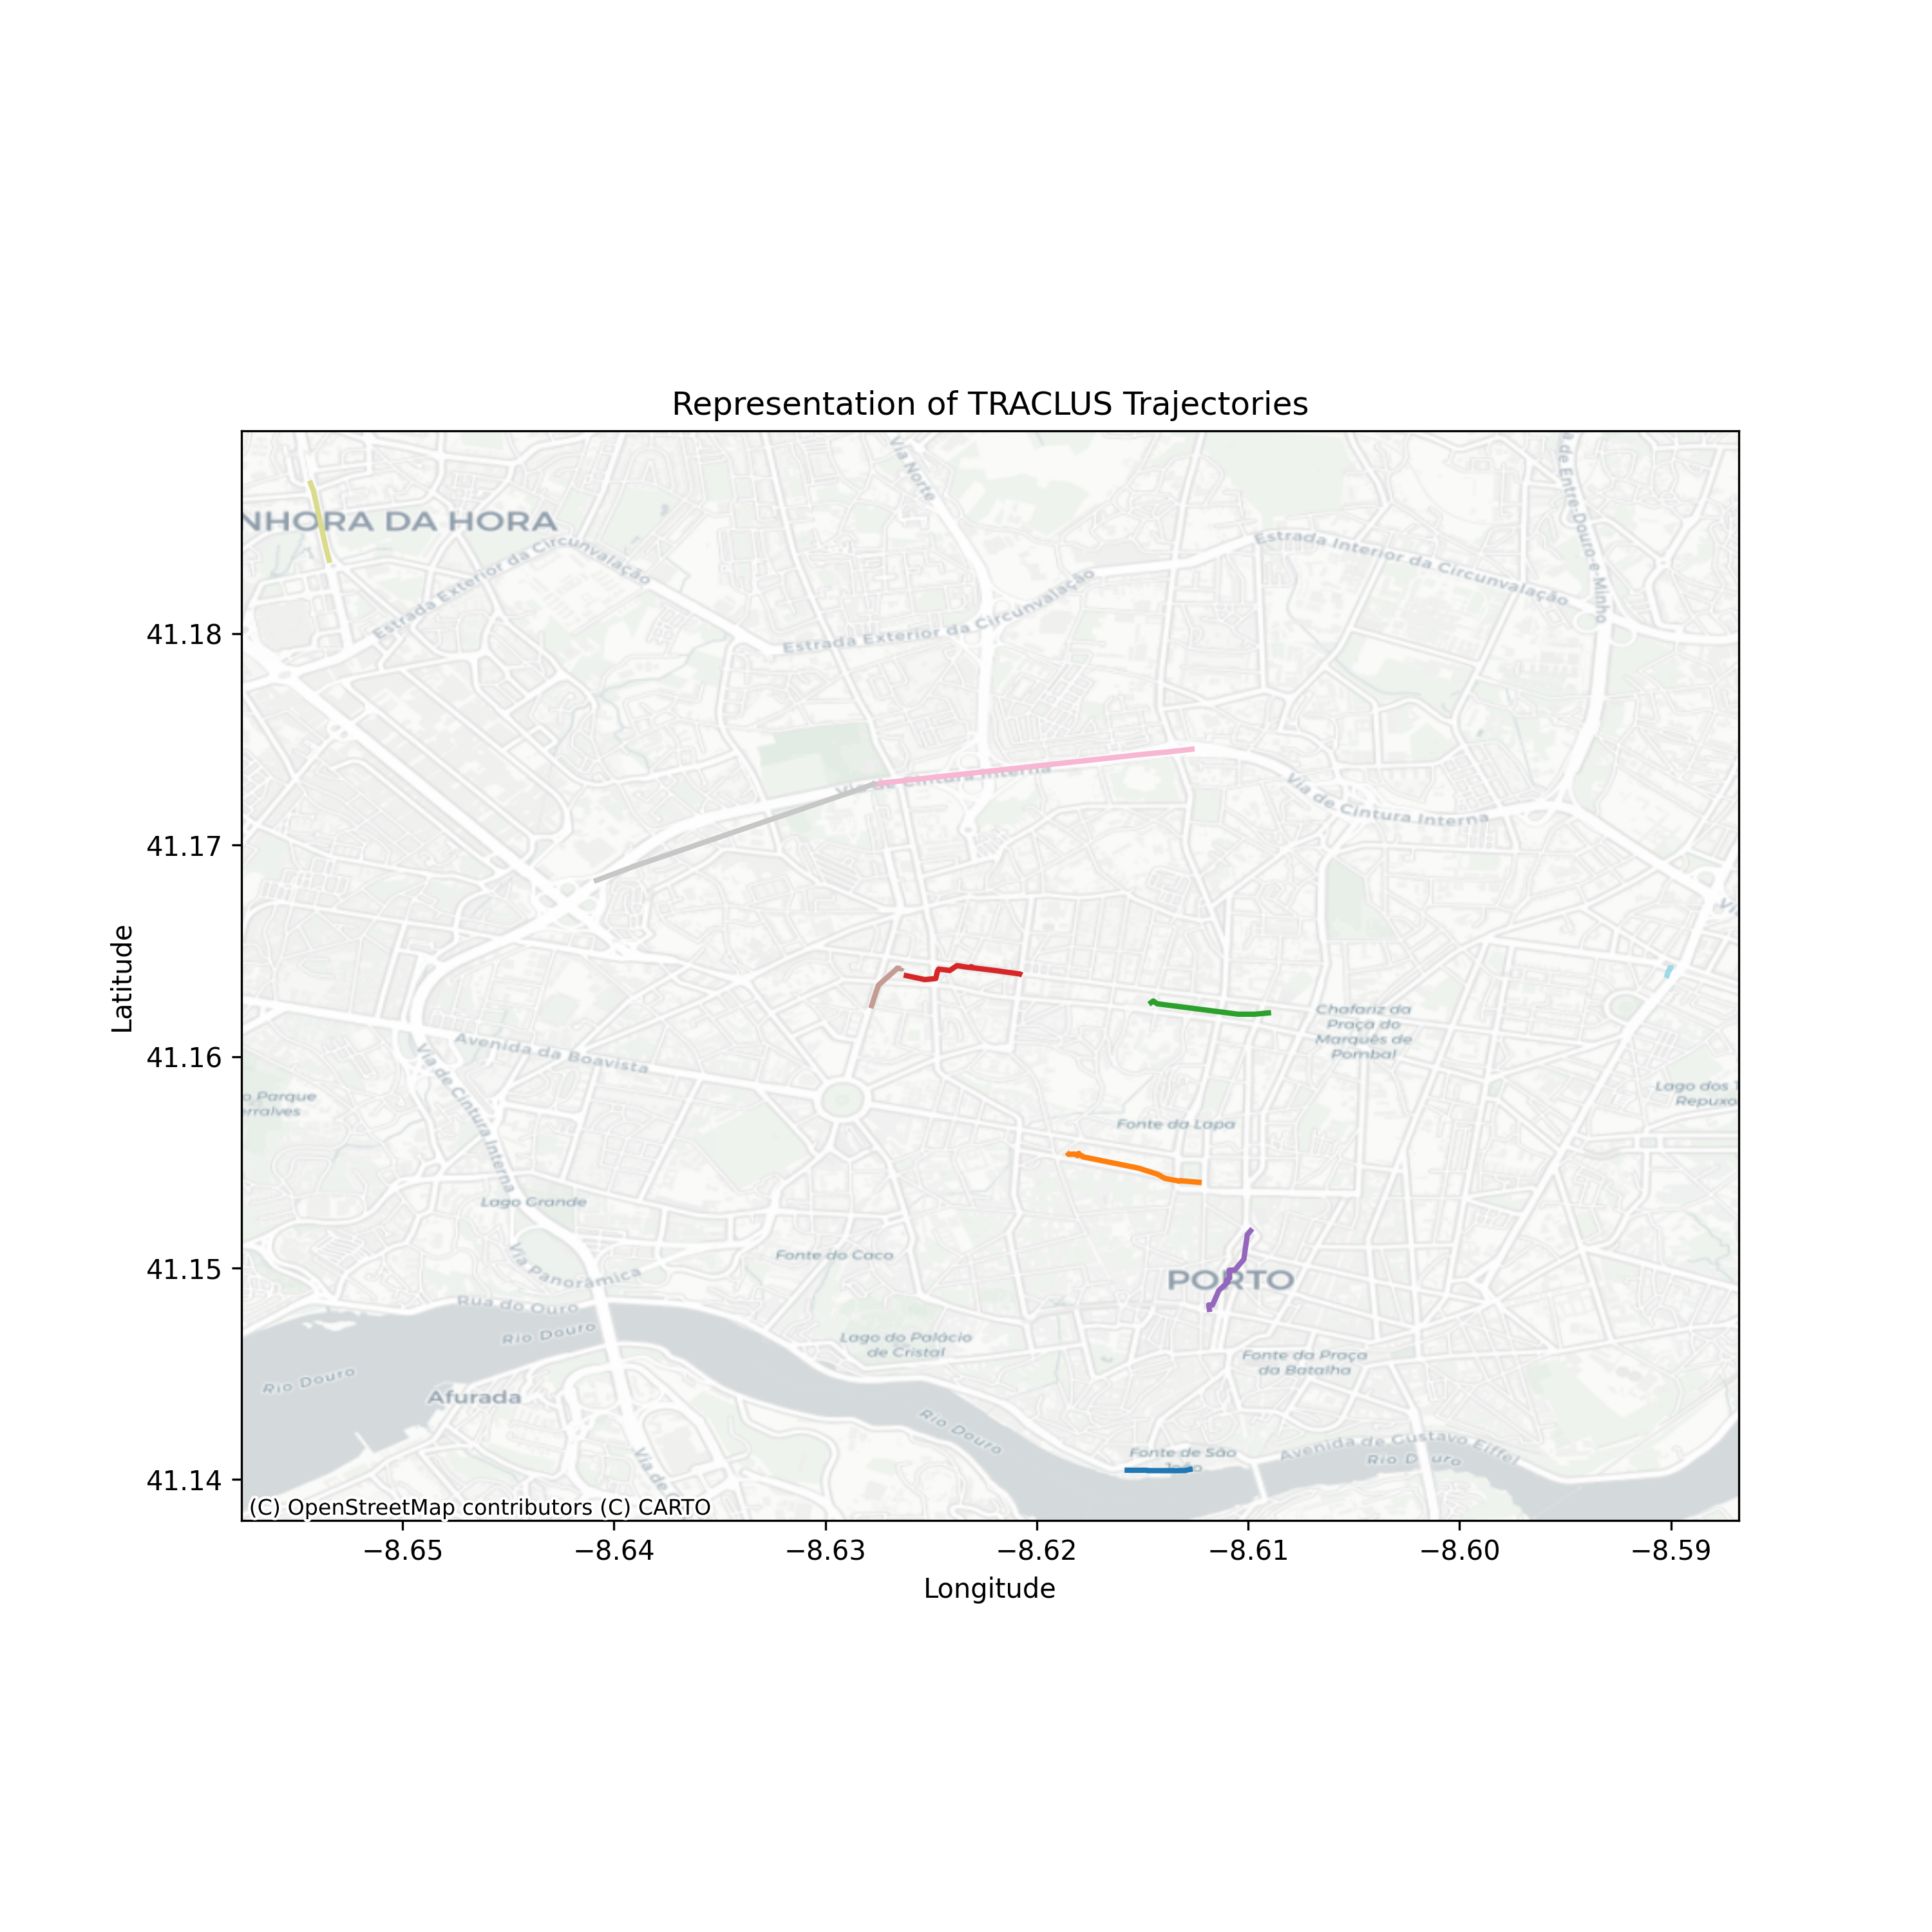
\includegraphics[width=0.5\textwidth]{img/Taxis/map_dbscan_auto.png}
    \caption{Resultados con todos los algoritmos en DBSCAN.}
    \label{fig:taxis_algorith_dbscan}
\end{figure}

\FloatBarrier

\begin{figure}[h!]
    \centering
    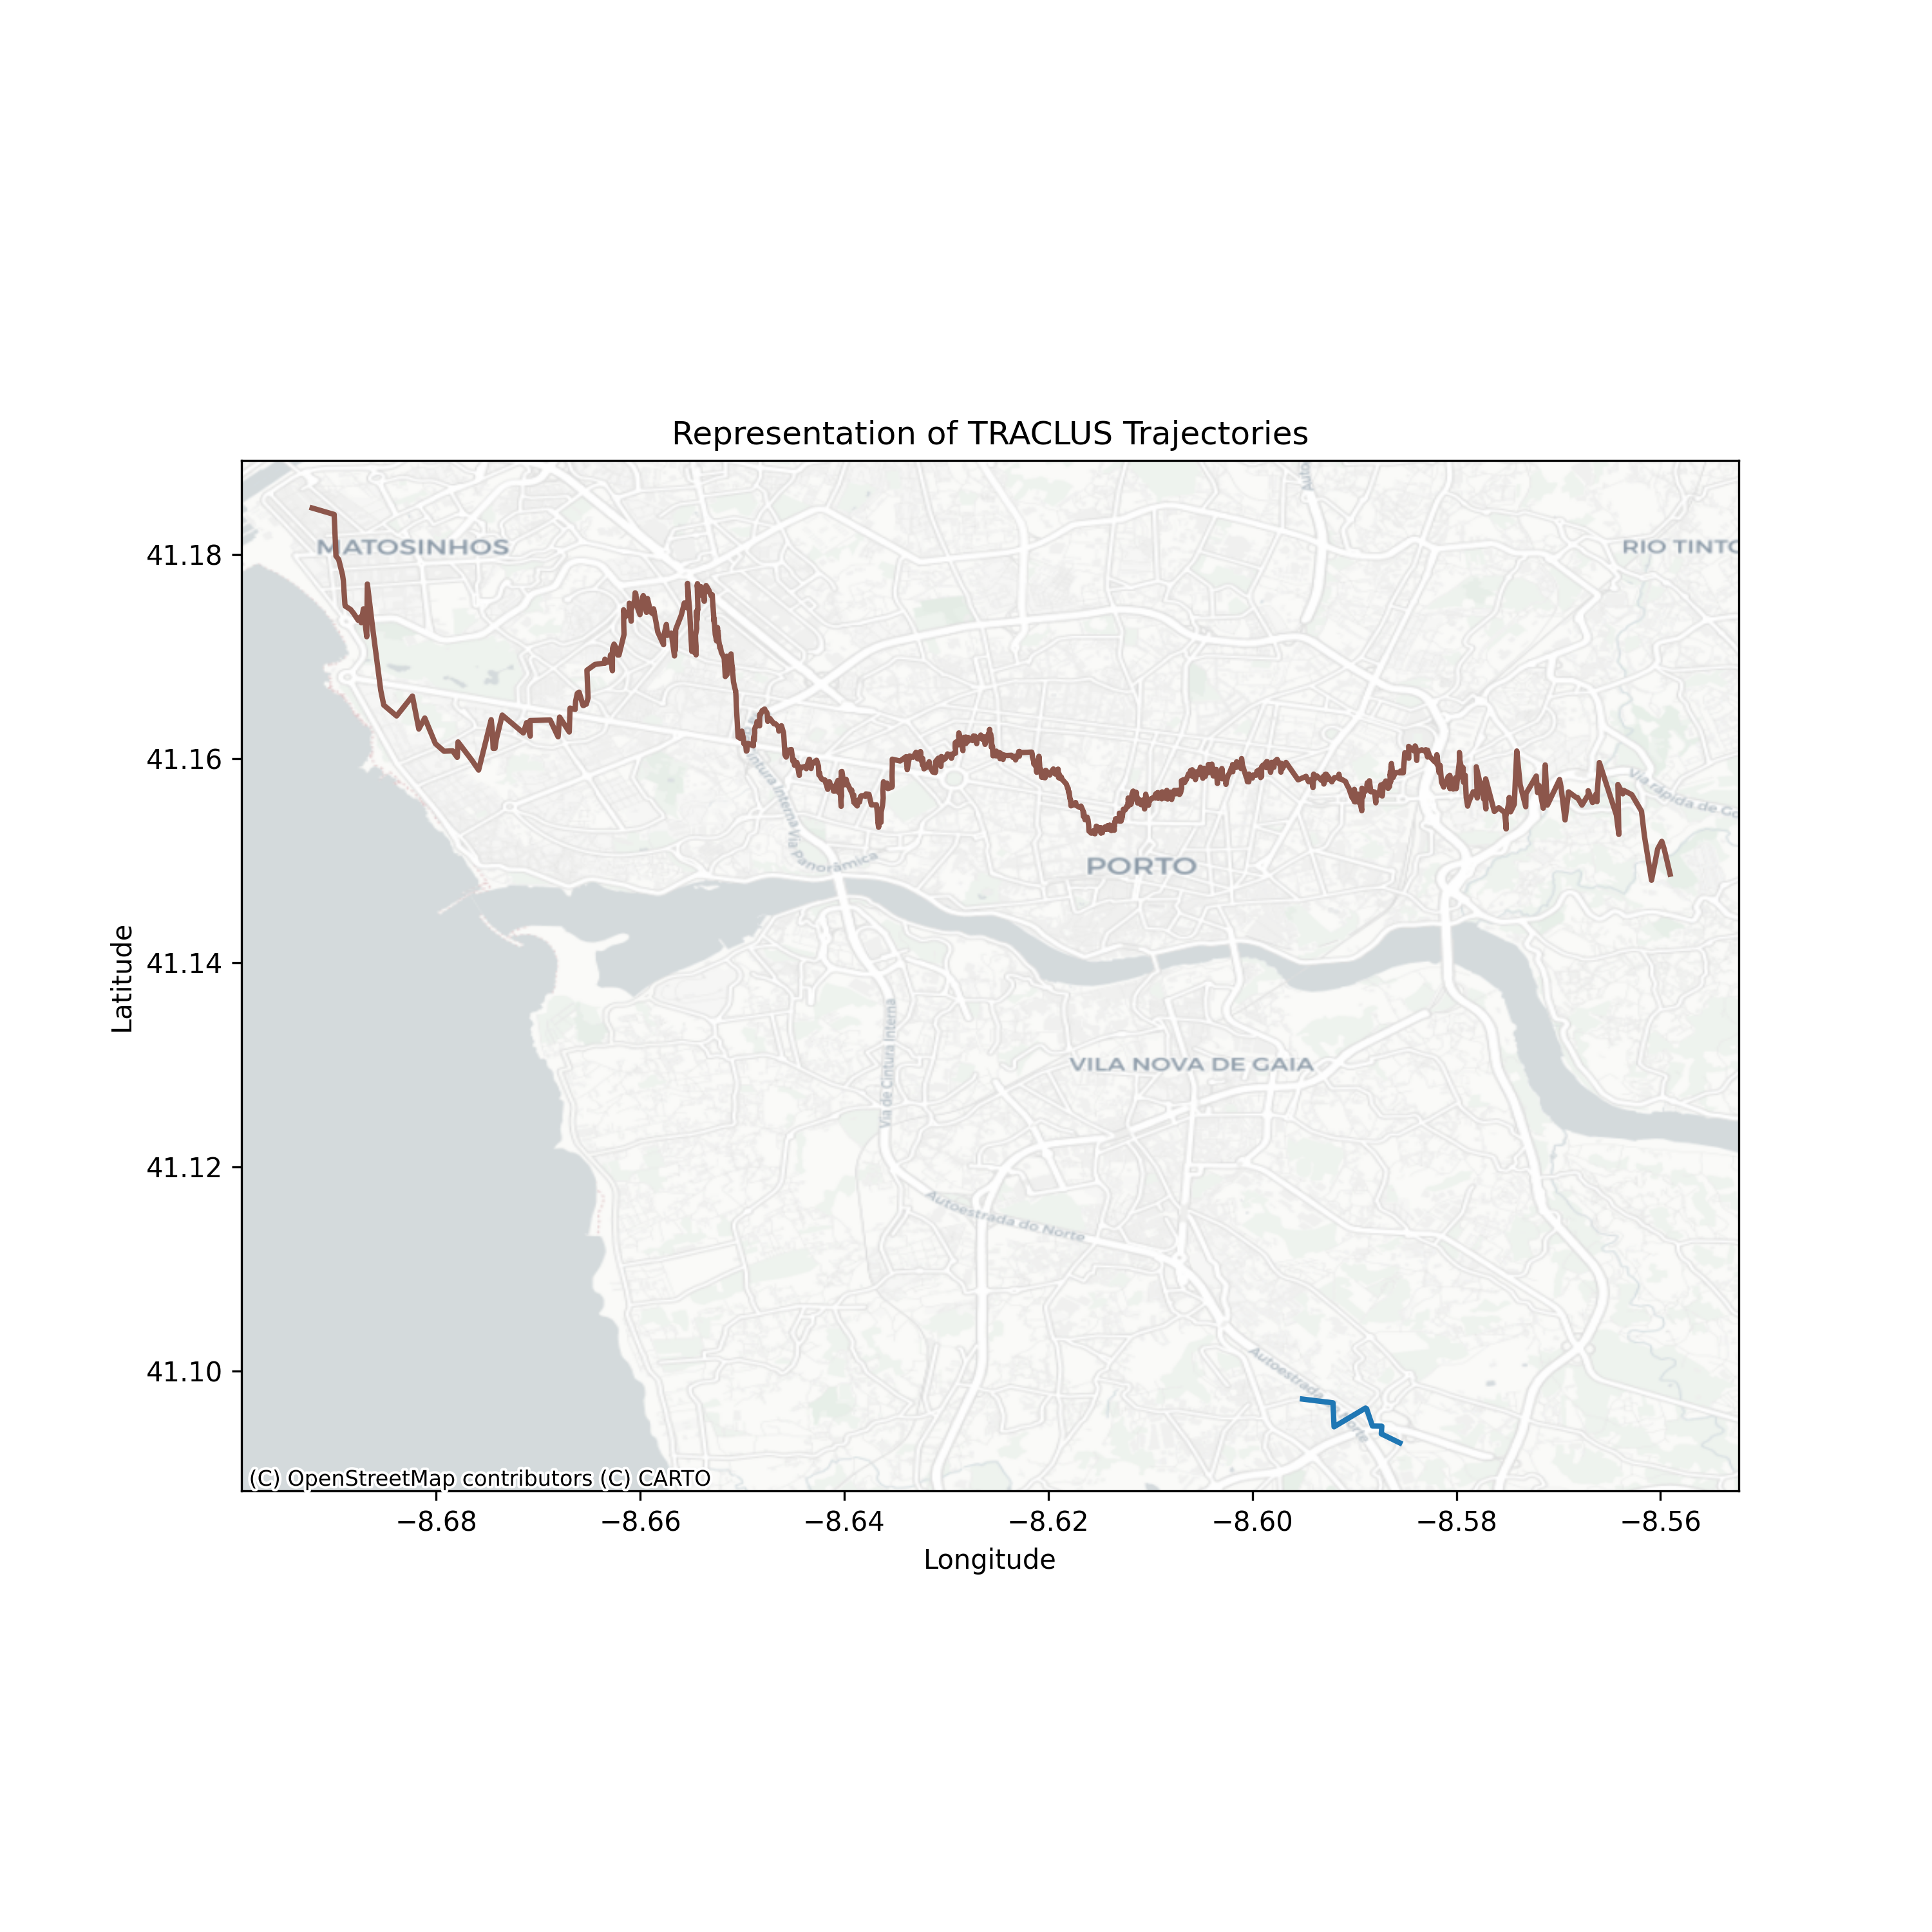
\includegraphics[width=0.5\textwidth]{img/Taxis/map_hdbscan_auto.png}
    \caption{Resultados con todos los algoritmos en HDBSCAN.}
    \label{fig:taxis_algorith_hdbscan}
\end{figure}

\FloatBarrier

De la misma forma que los resultados eran afectados por los algoritmos en este conjunto lo fueran en los demás.

- \textbf{Conjunto Movebank}: 


\begin{figure}[h!]
    \centering
    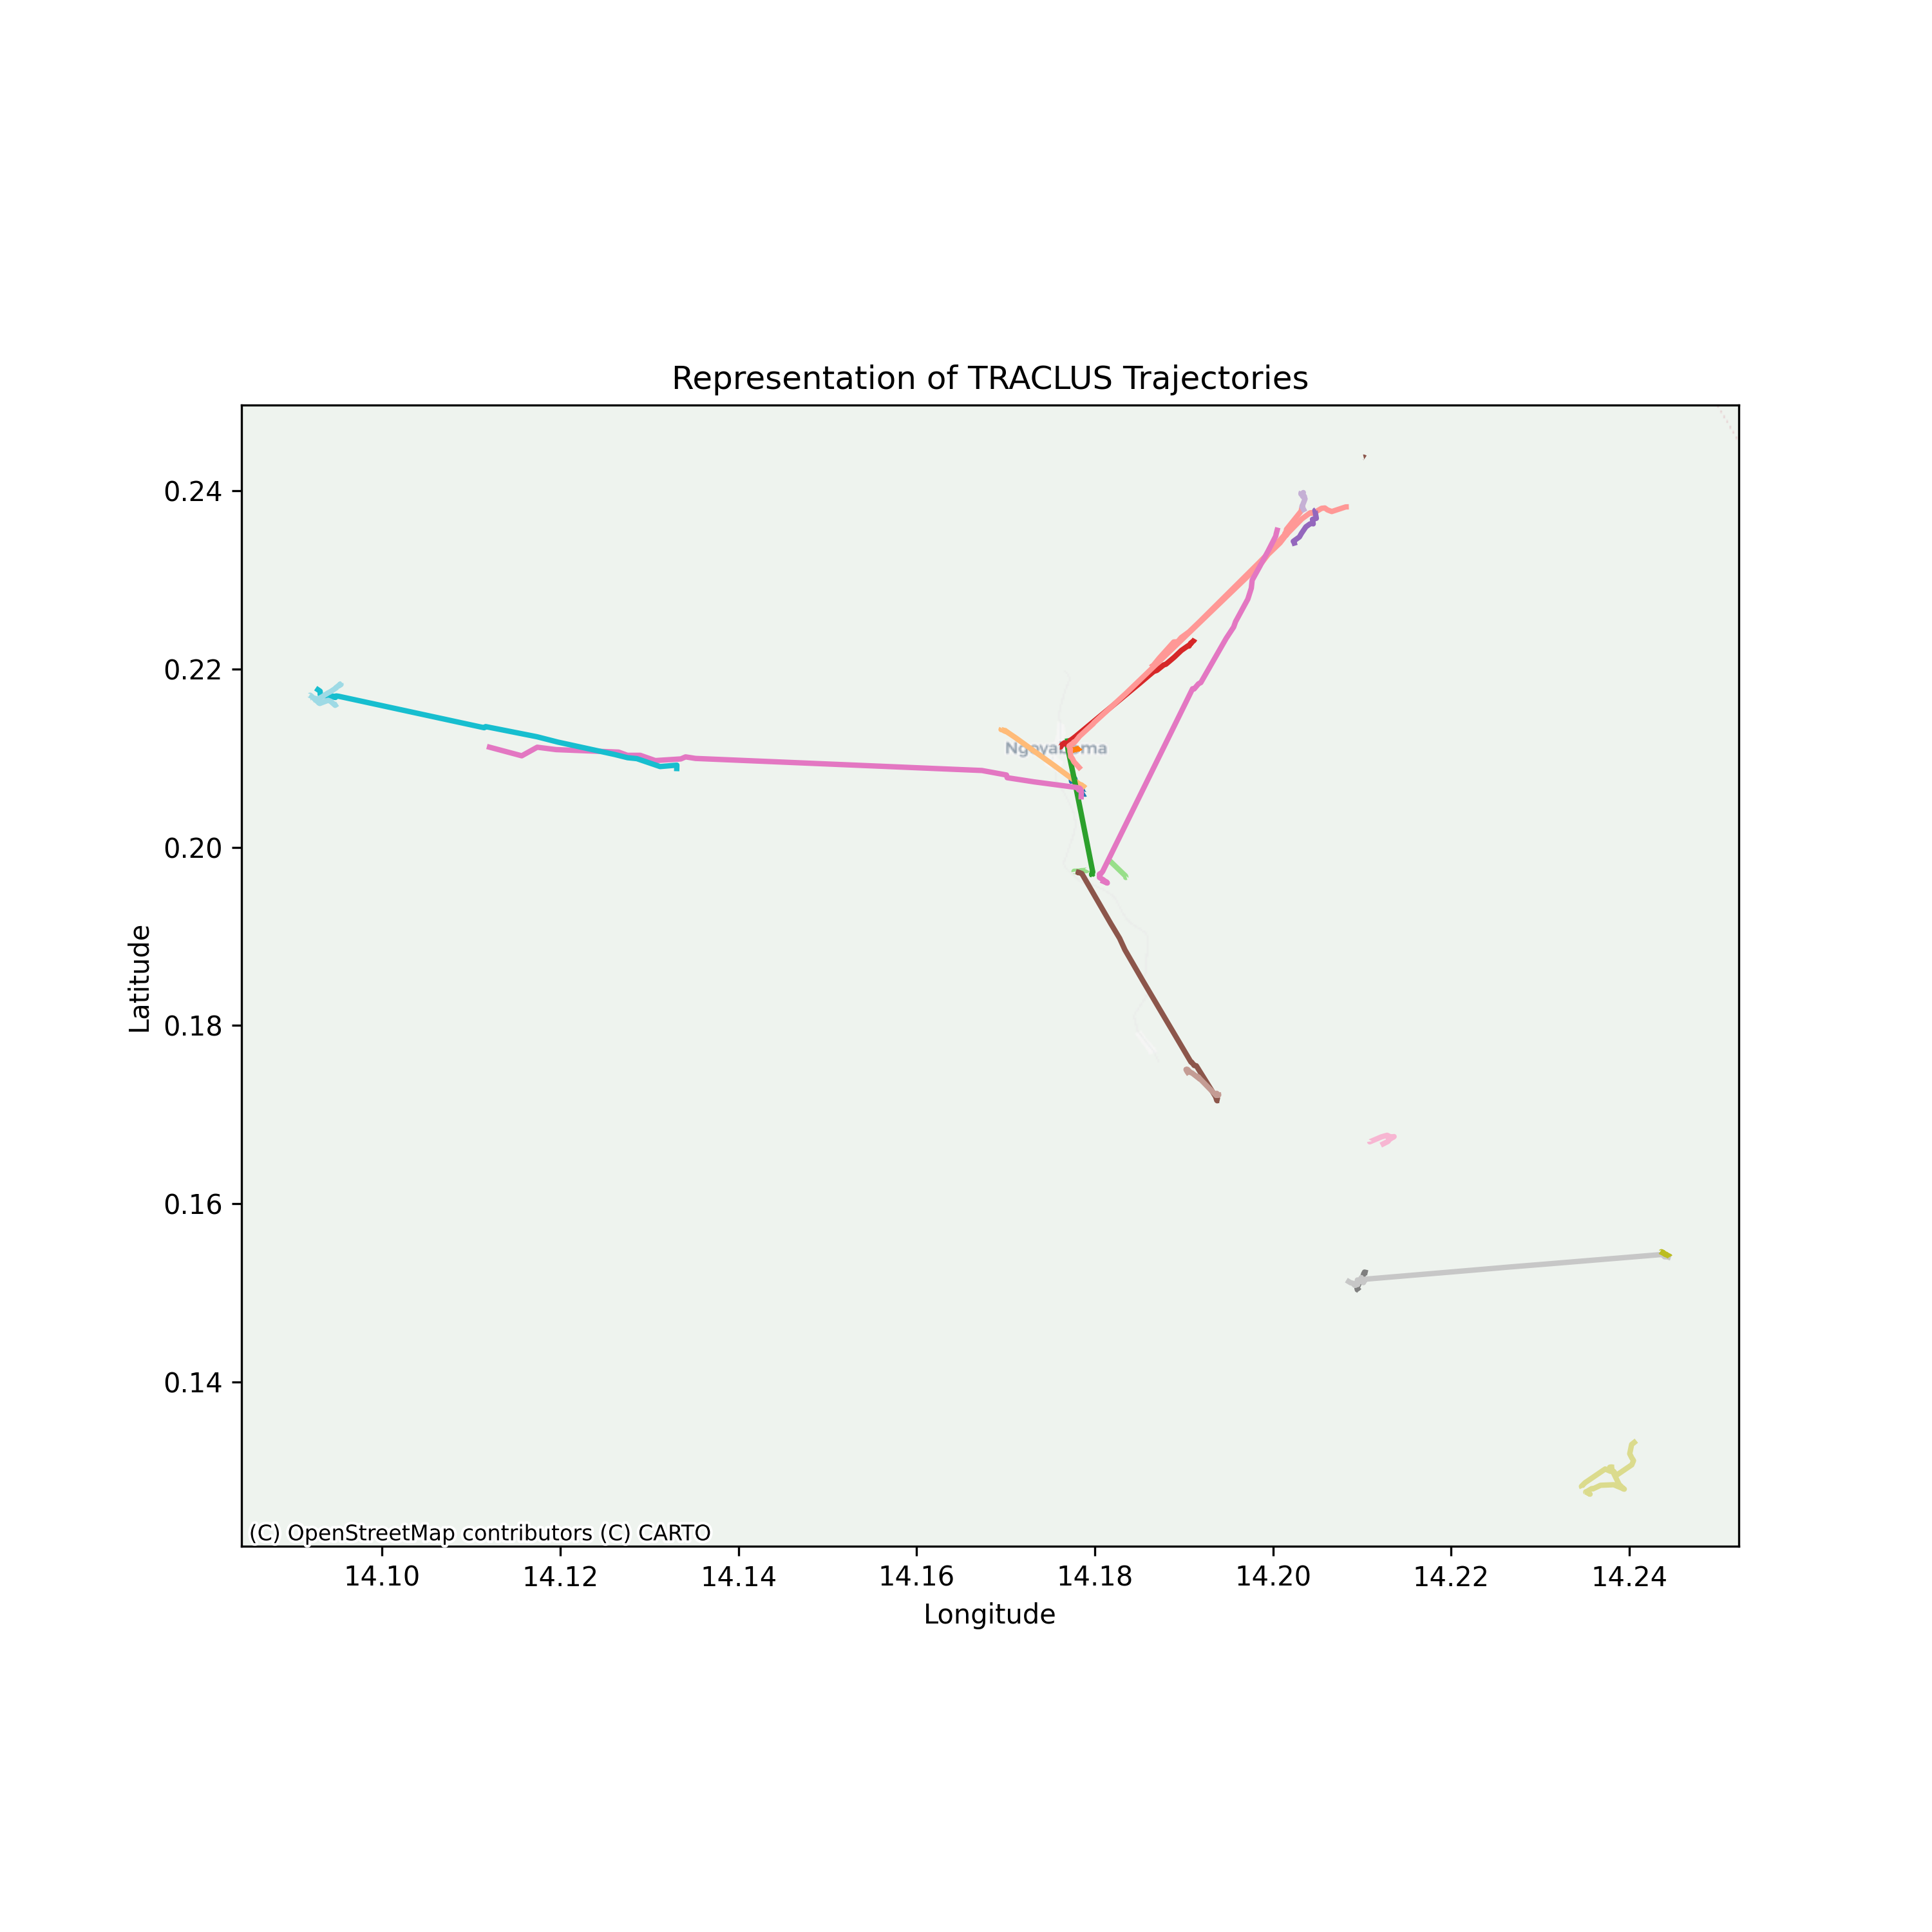
\includegraphics[width=0.5\textwidth]{img/Movebank/map_optics_auto.png}
    \caption{Resultados con todos los algoritmos en OPTICS y HDBSCAN.}
    \label{fig:movebank_algorith_optics}
\end{figure}

\FloatBarrier

\begin{figure}[h!]
    \centering
    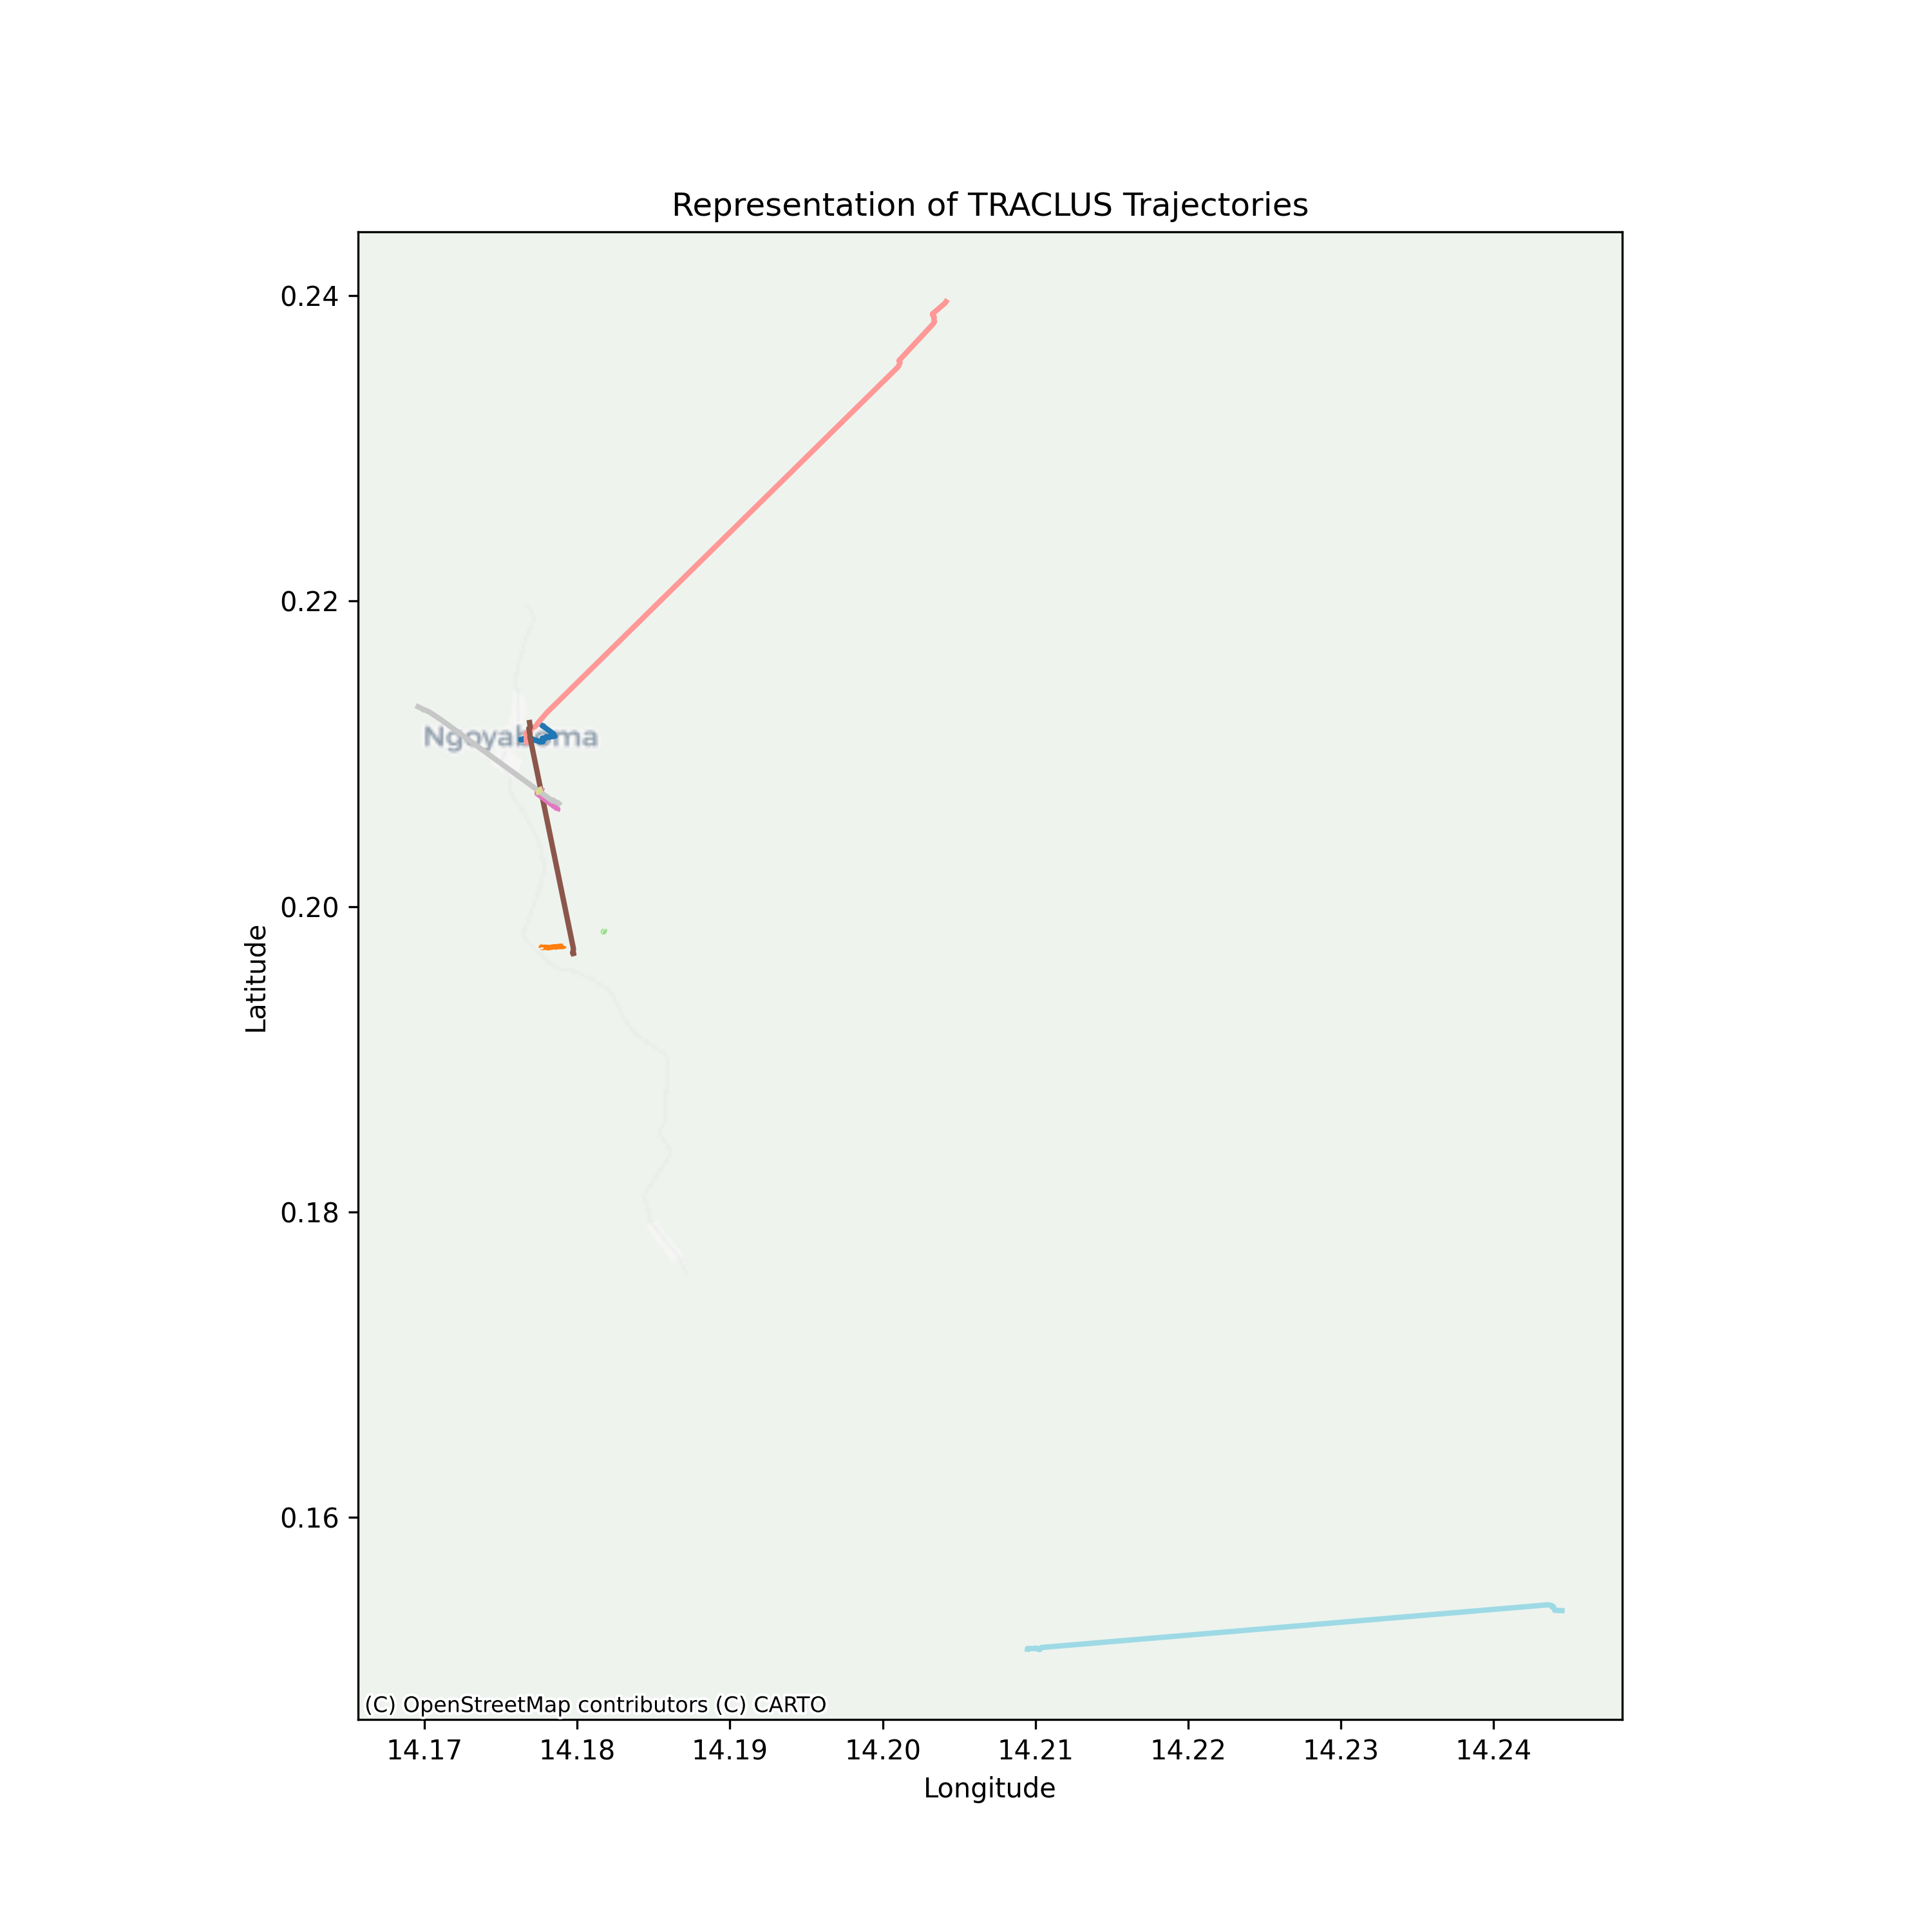
\includegraphics[width=0.5\textwidth]{img/Movebank/map_dbscan_auto.png}
    \caption{Resultados con todos los algoritmos en DBSCAN.}
    \label{fig:movebank_algorith_dbscan}
\end{figure}

\FloatBarrier

\begin{figure}[h!]
    \centering
    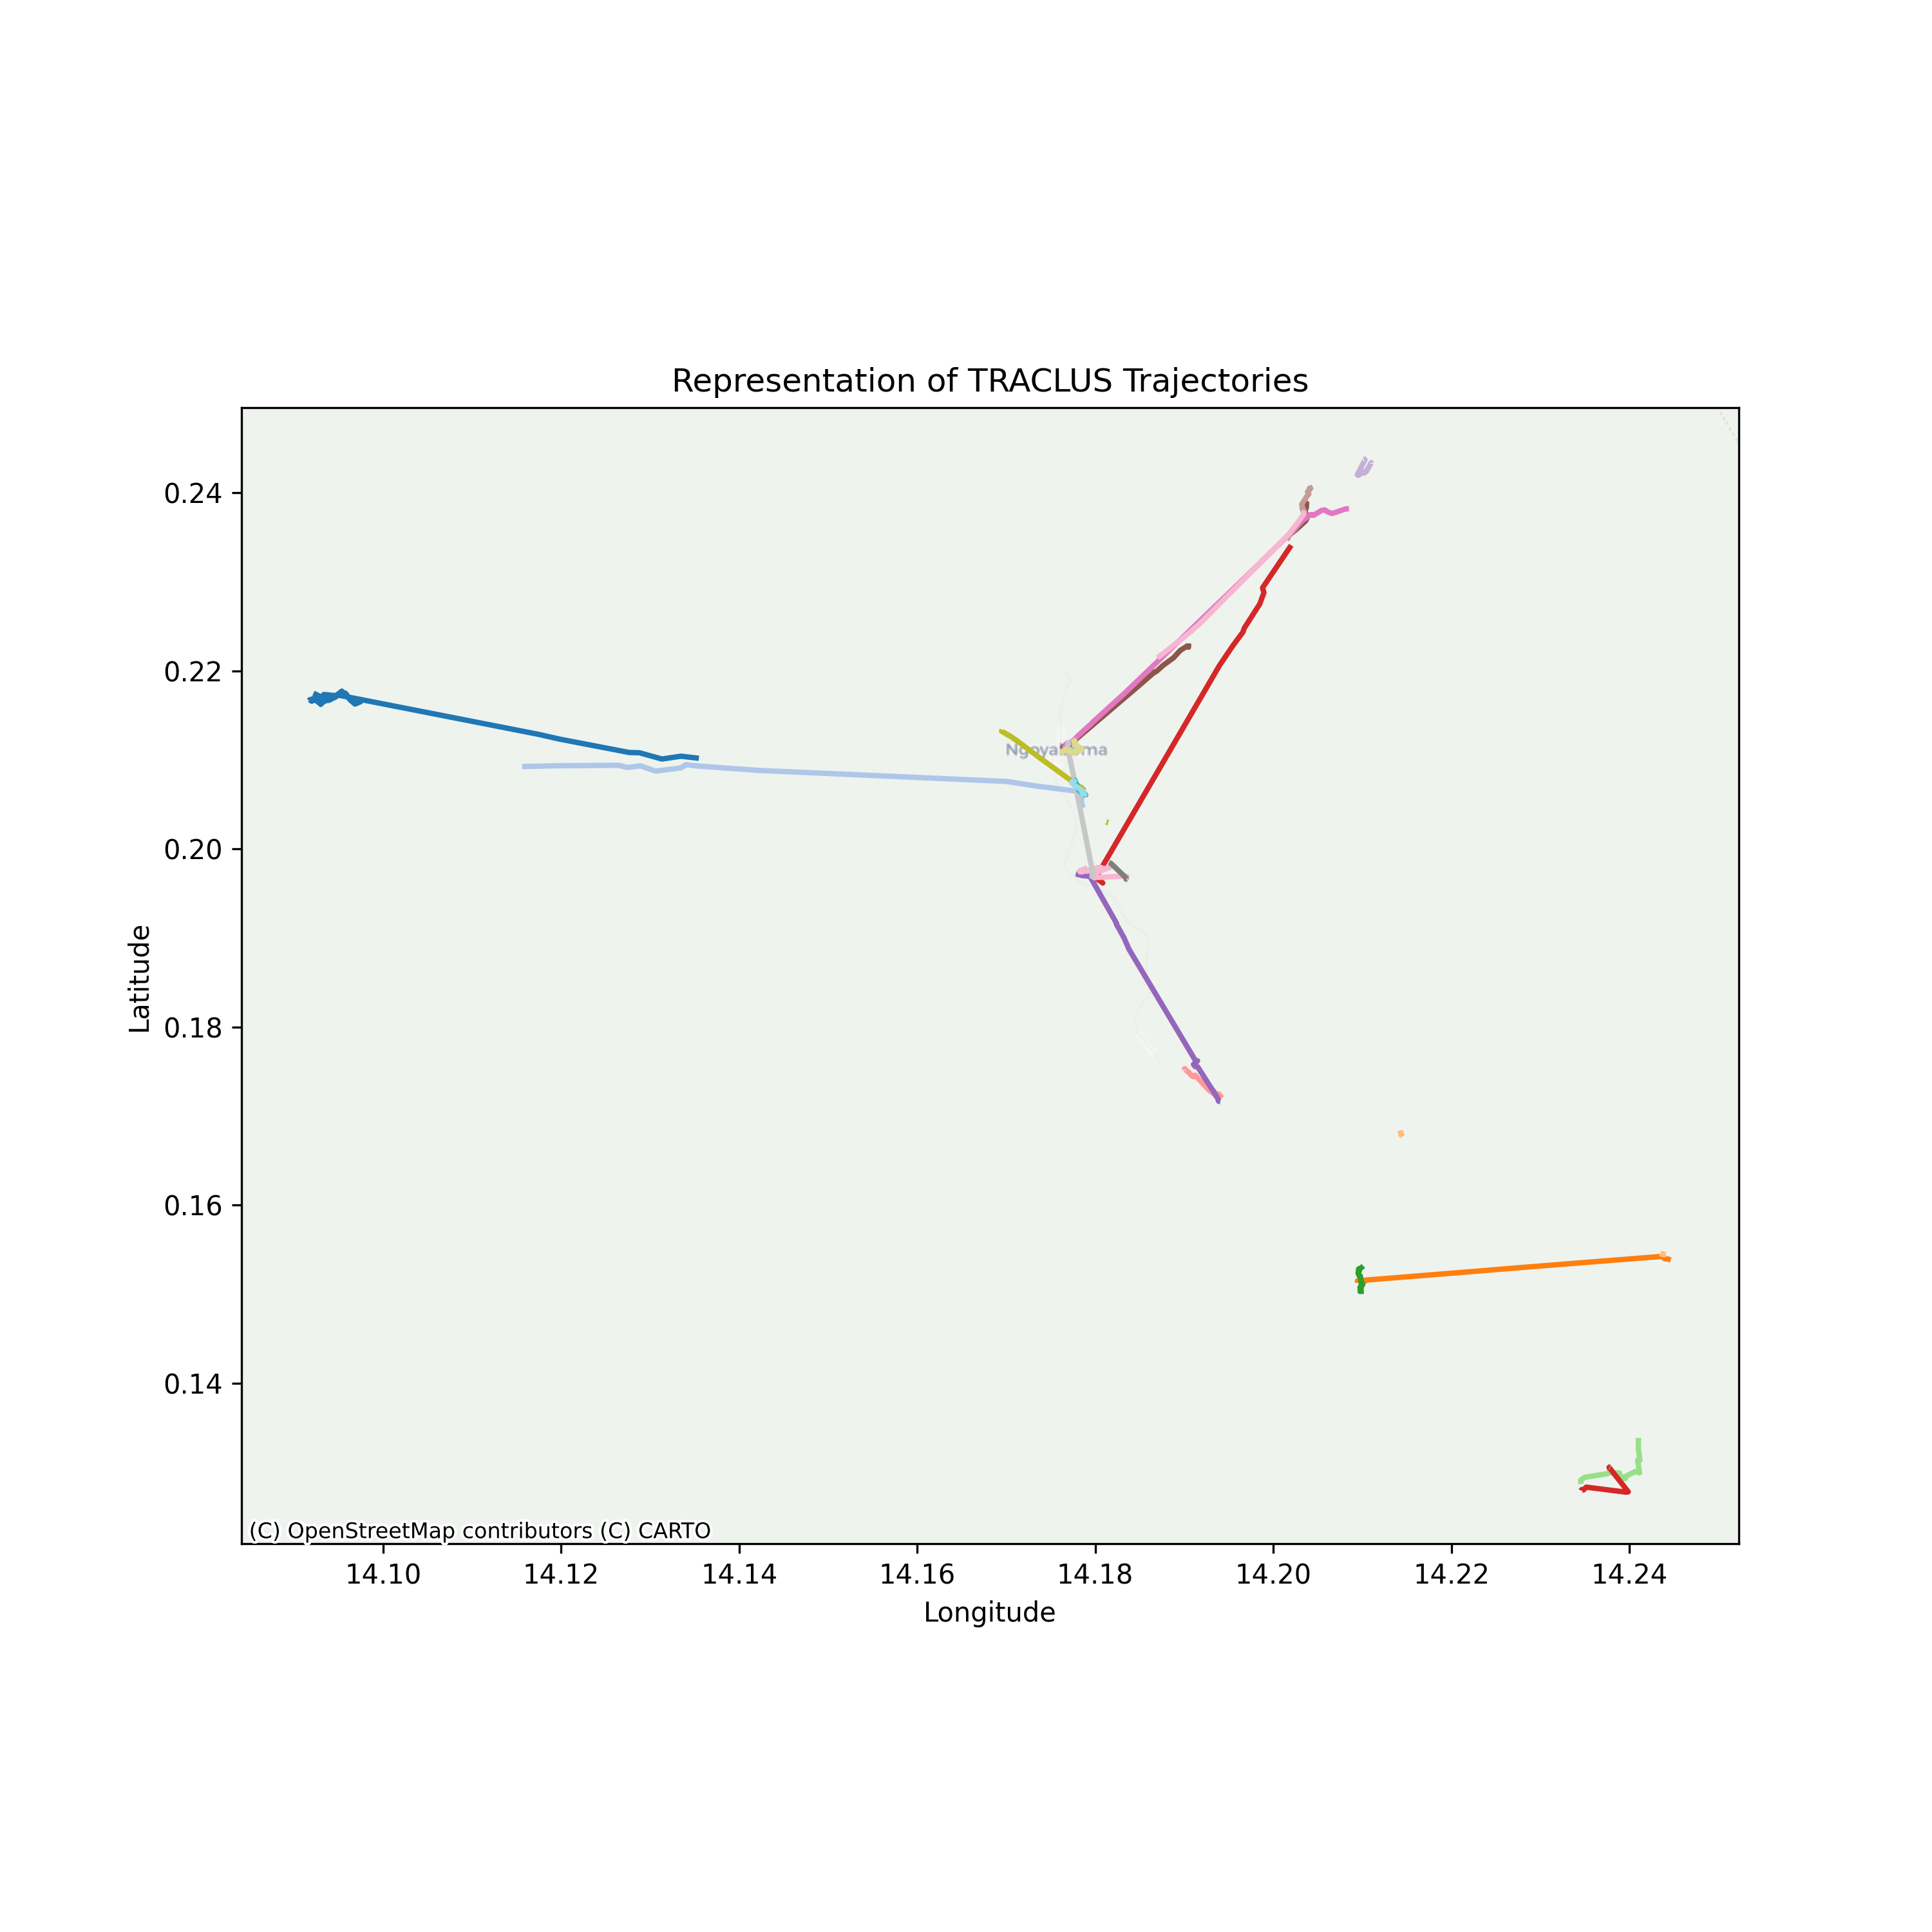
\includegraphics[width=0.5\textwidth]{img/Movebank/map_hdbscan_auto.png}
    \caption{Resultados con todos los algoritmos en HDBSCAN.}
    \label{fig:movebank_algorith_hdbscan}
\end{figure}

\FloatBarrier

- \textbf{Conjunto Geolife}: 


\begin{figure}[h!]
    \centering
    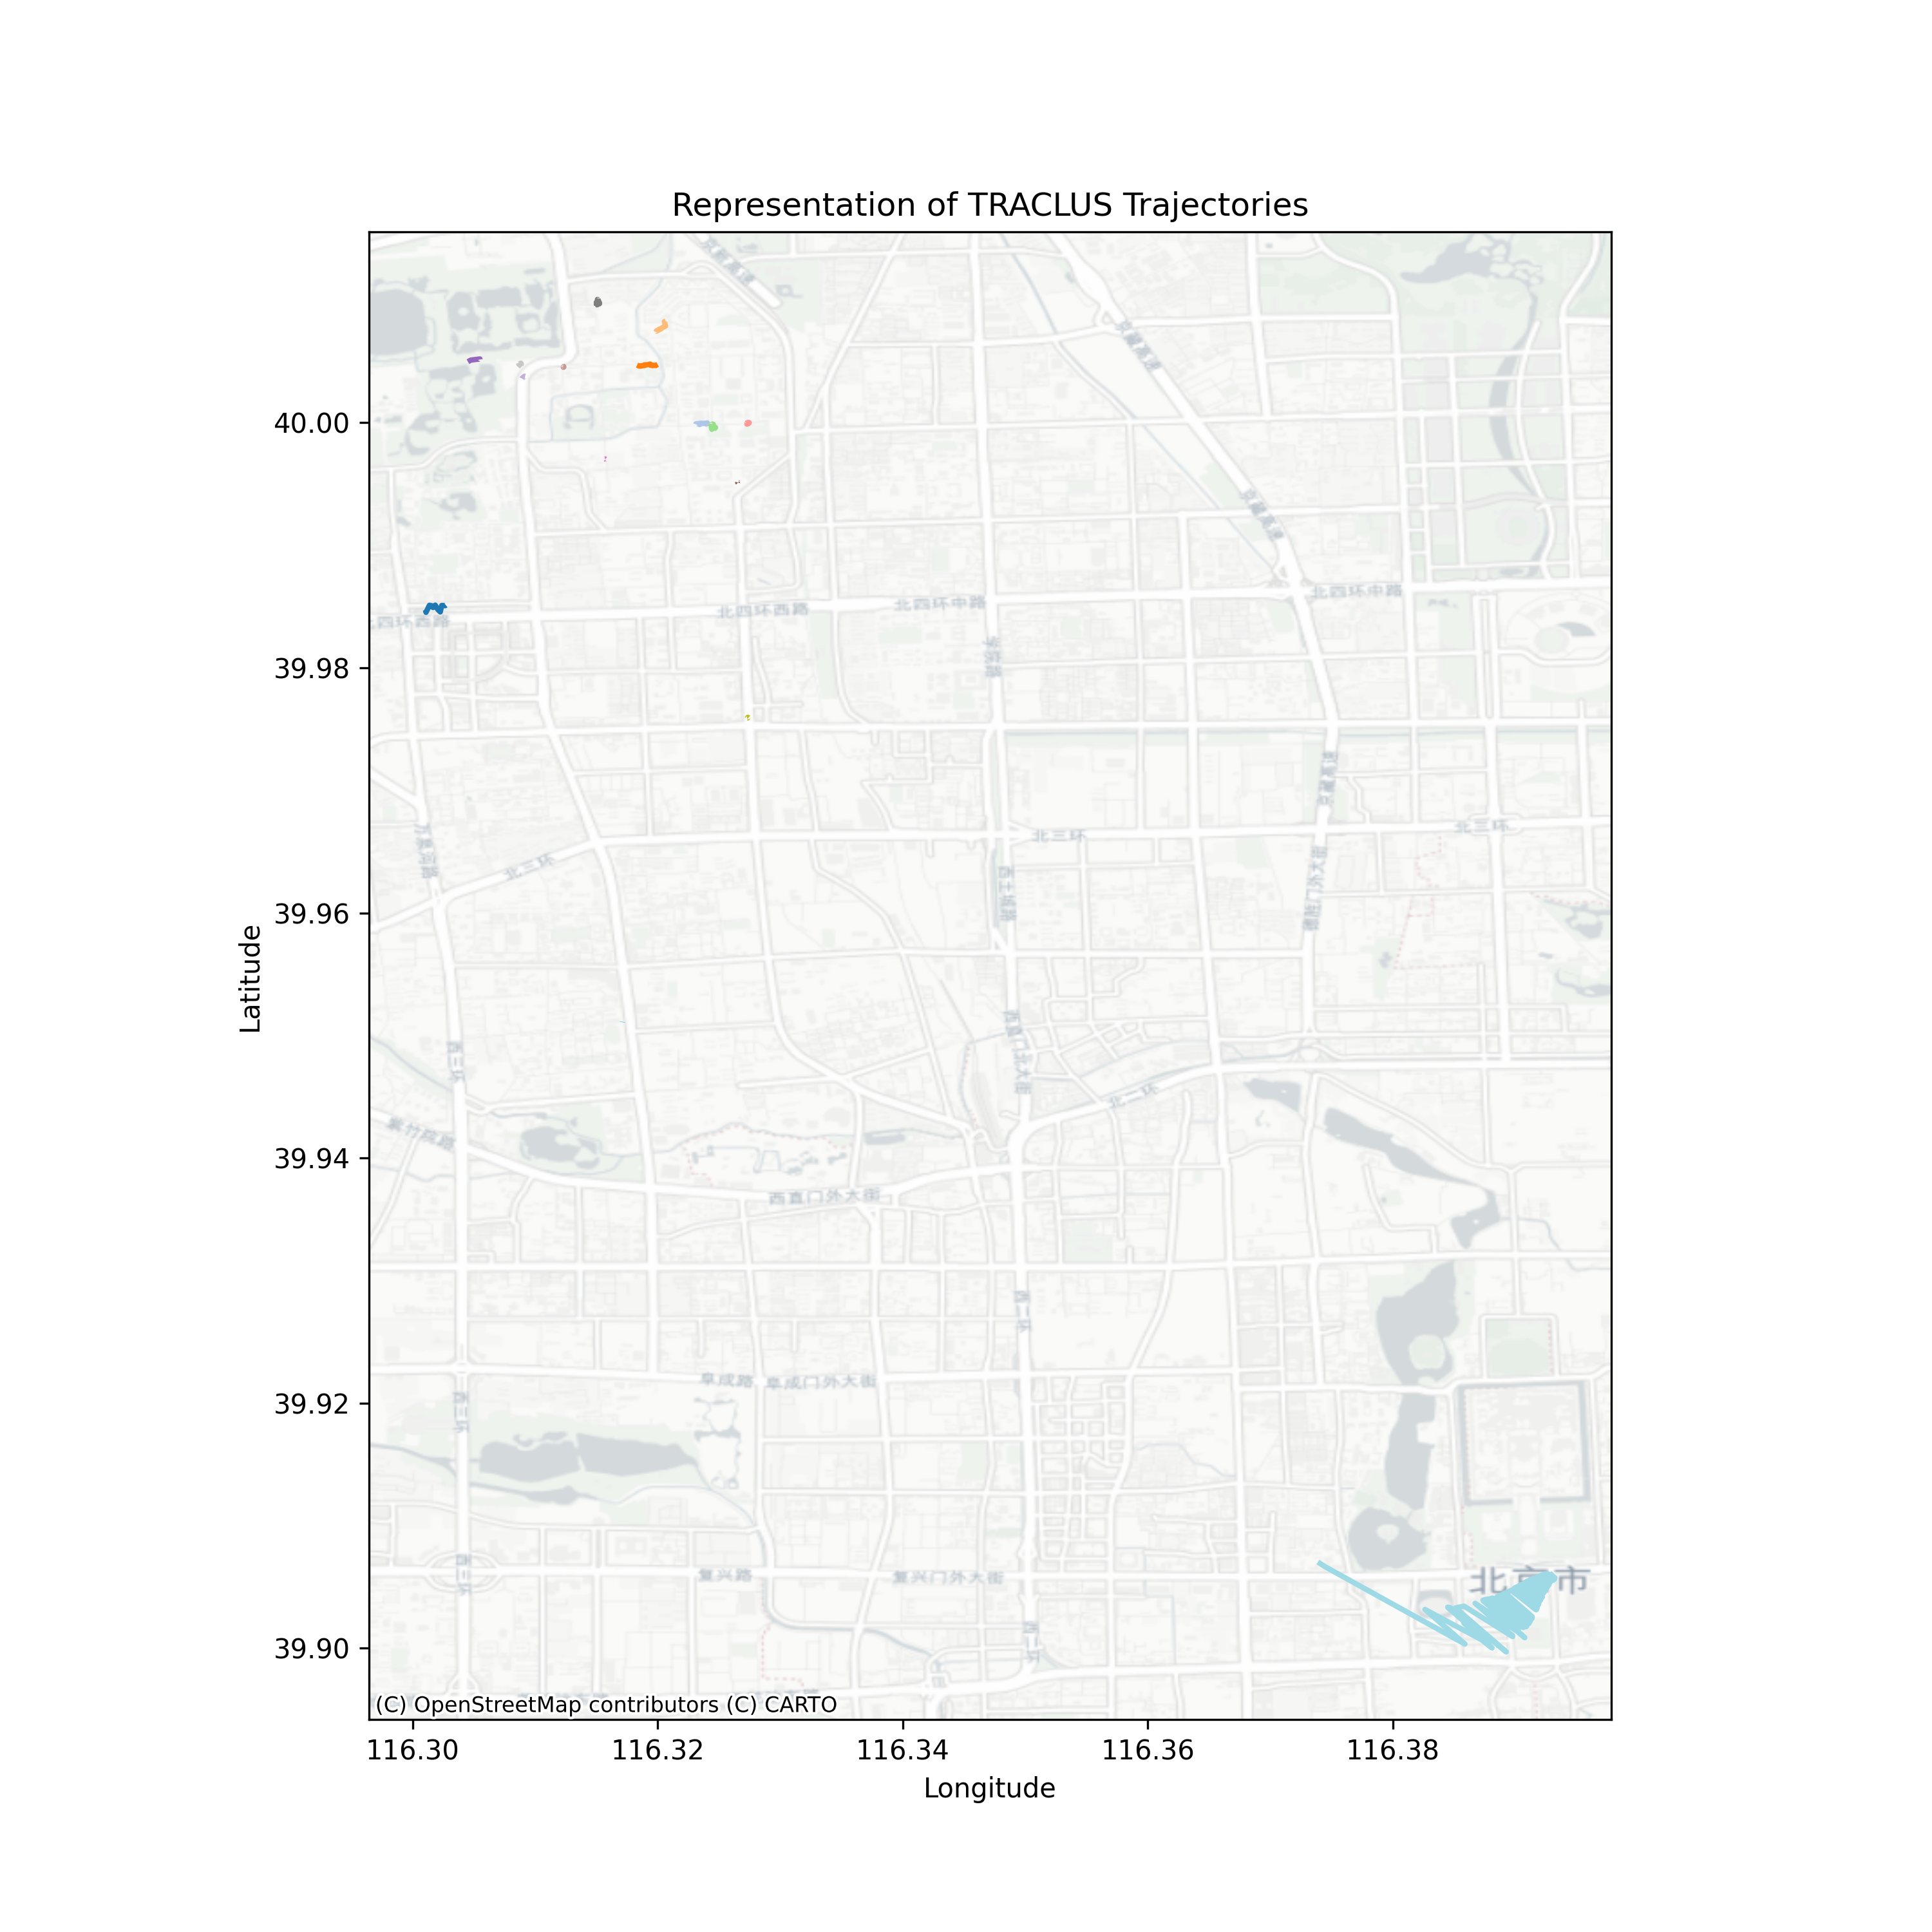
\includegraphics[width=0.5\textwidth]{img/Geolife/map_optics_auto.png}
    \caption{Resultados con todos los algoritmos en OPTICS.}
    \label{fig:geolife_algorith_optics}
\end{figure}

\FloatBarrier

\begin{figure}[h!]
    \centering
    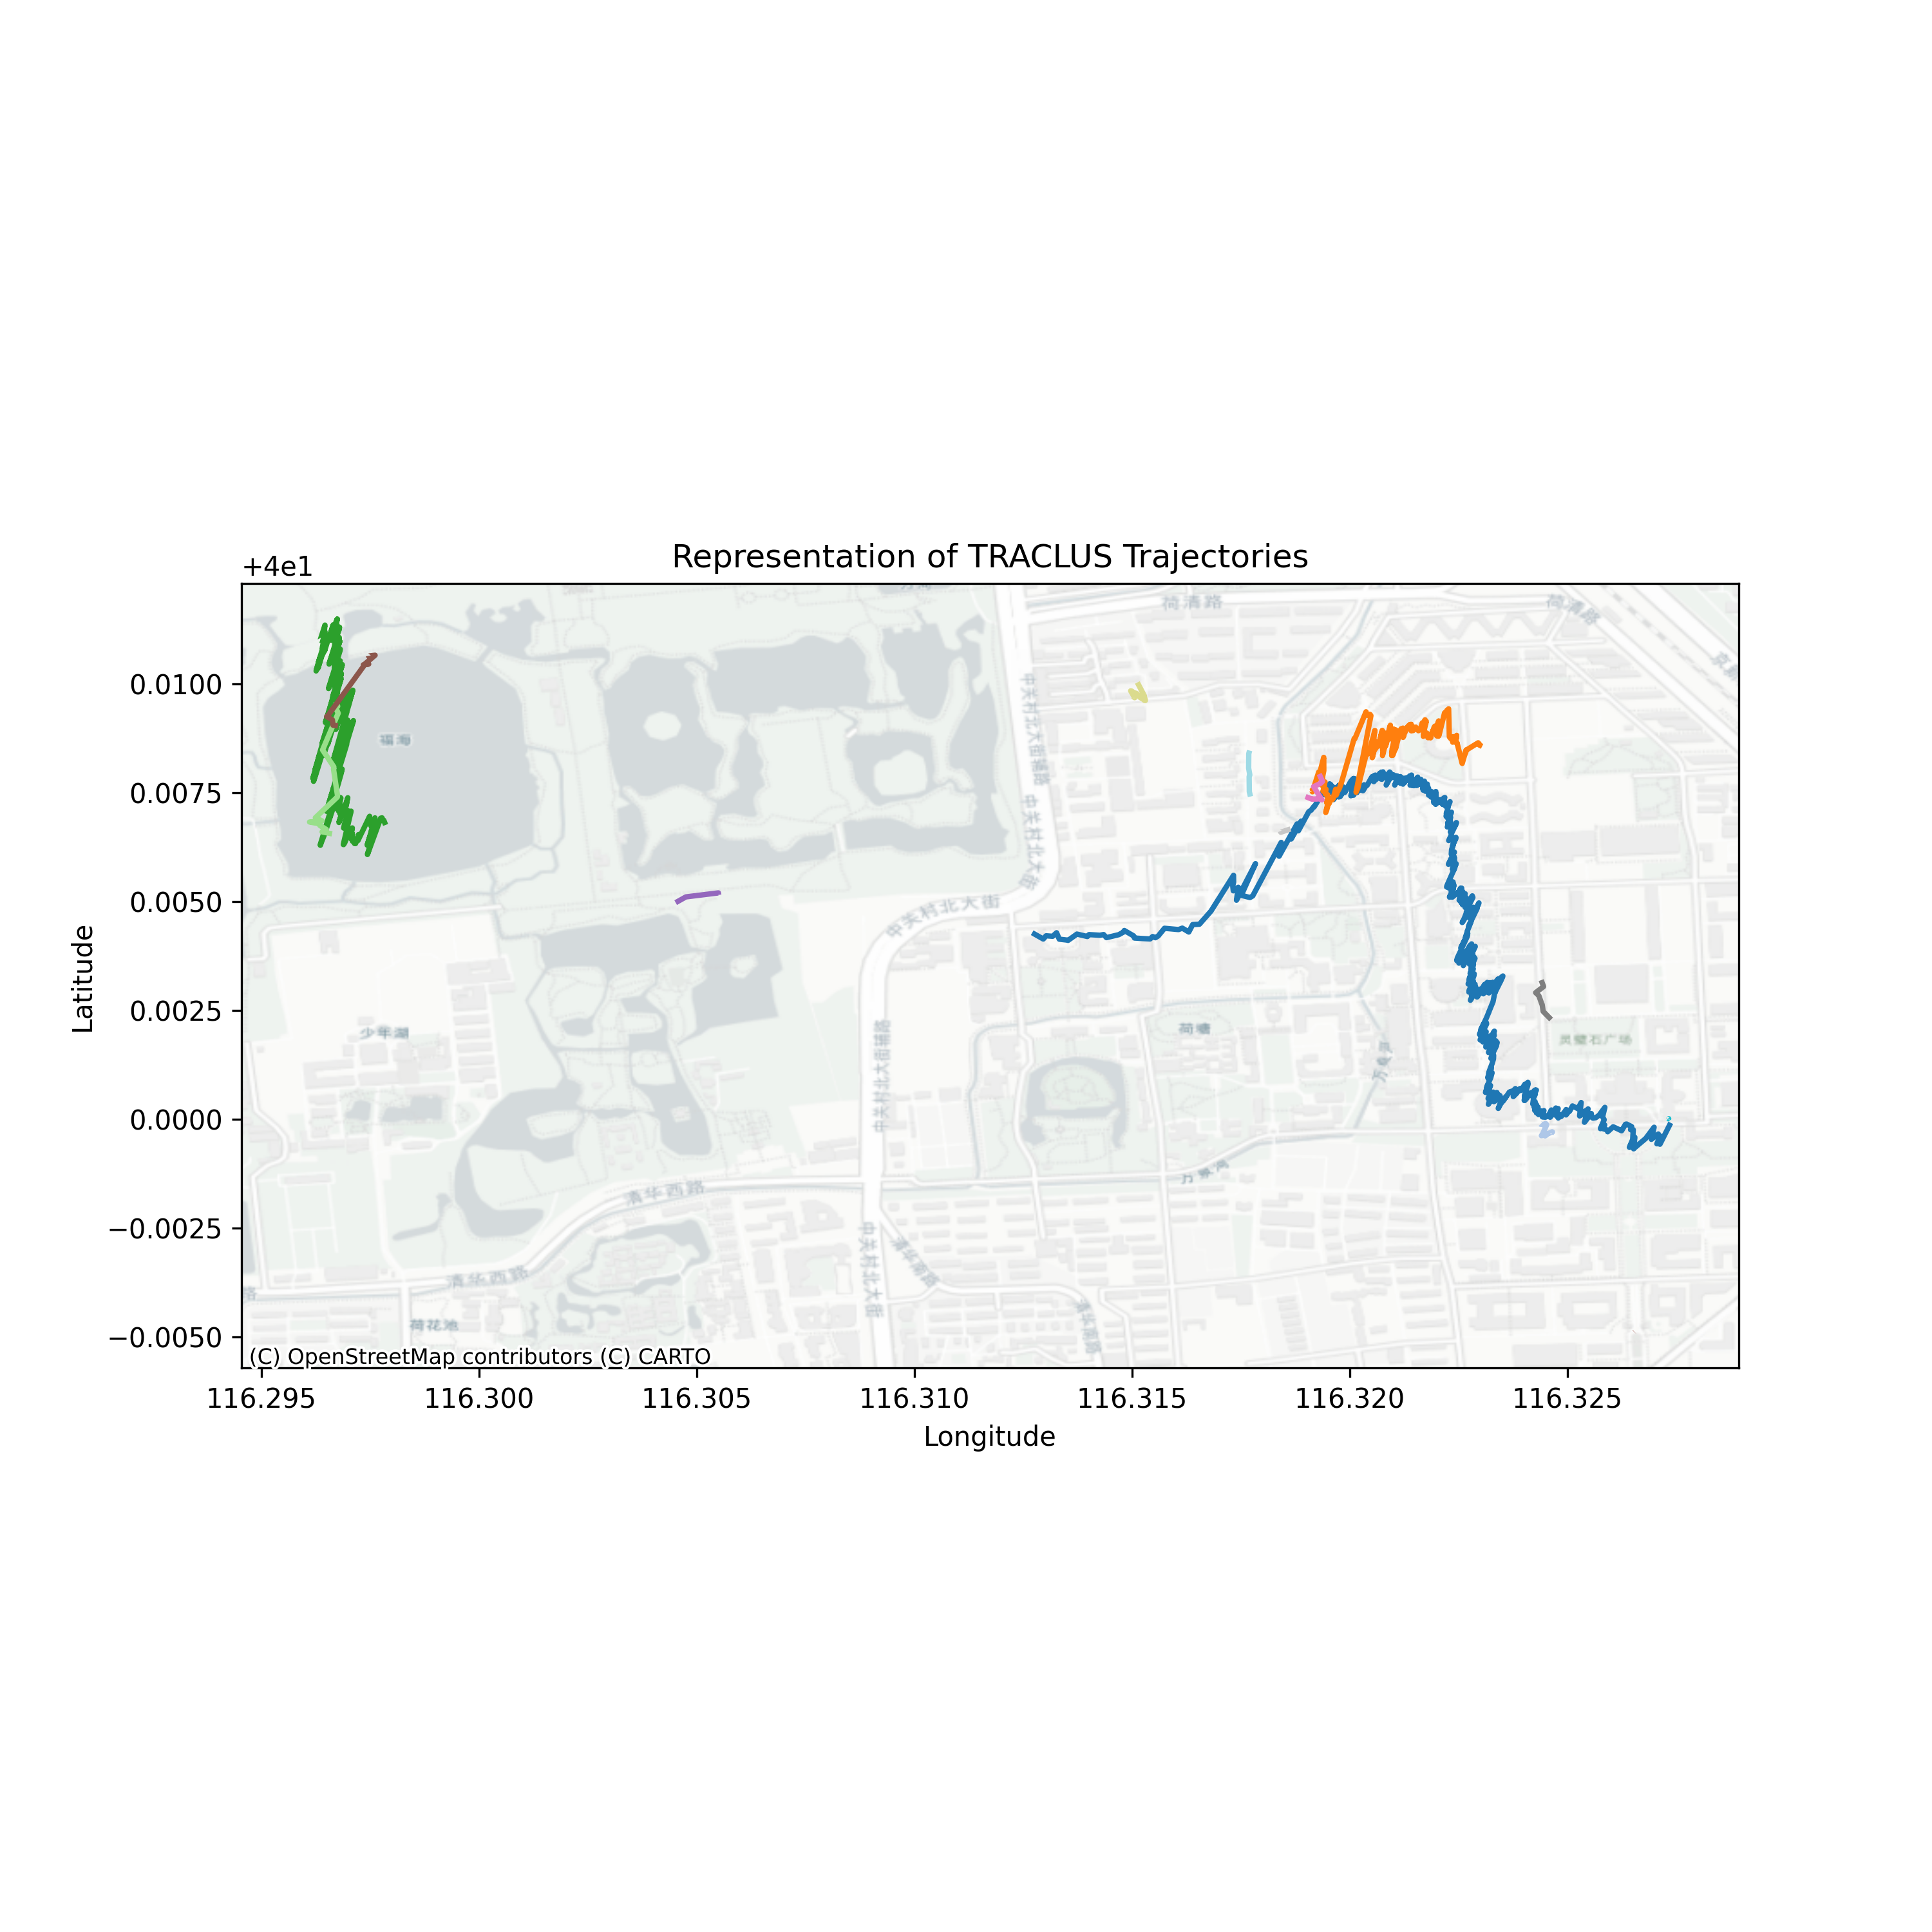
\includegraphics[width=0.5\textwidth]{img/Geolife/map_dbscan_auto.png}
    \caption{Resultados con todos los algoritmos en DBSCAN.}
    \label{fig:geolife_algorith_dbscan}
\end{figure}

\FloatBarrier

\begin{figure}[h!]
    \centering
    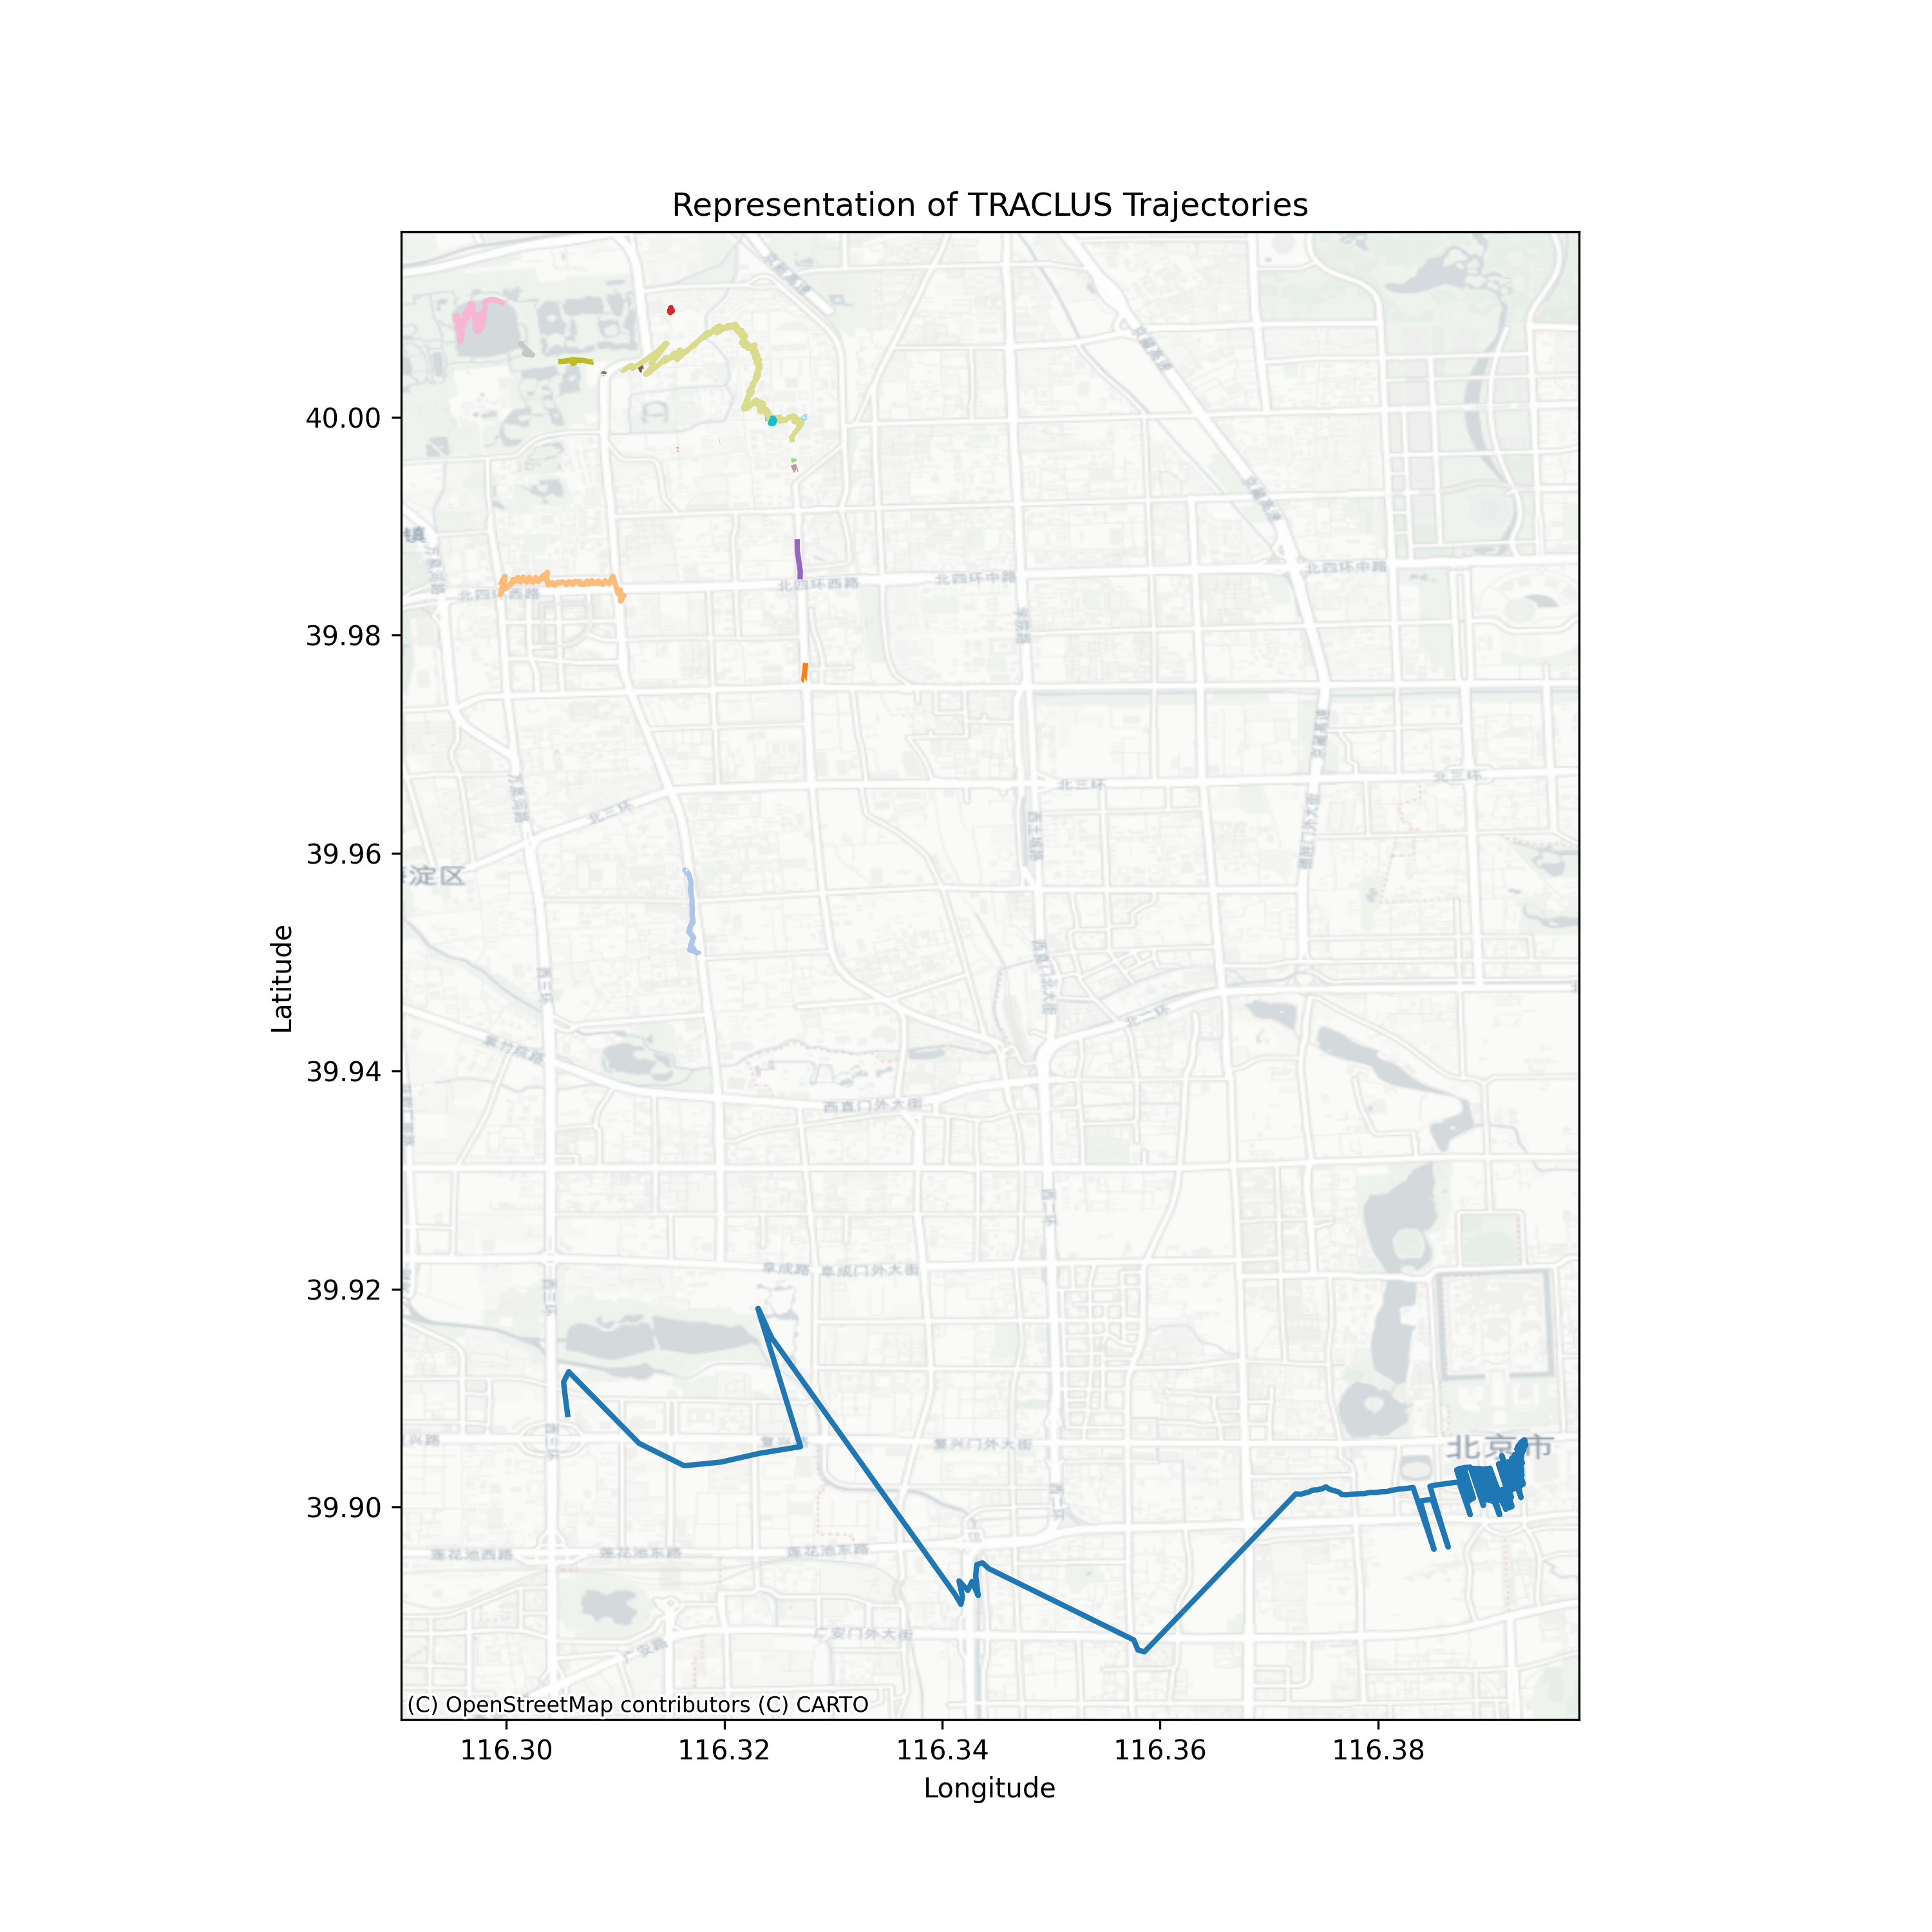
\includegraphics[width=0.5\textwidth]{img/Geolife/map_hdbscan_auto.png}
    \caption{Resultados con todos los algoritmos en HDBSCAN.}
    \label{fig:geolife_algorith_hdbscan}
\end{figure}

\FloatBarrier

La comparacion no es totalmente adecuada ya que aunque se haya usado el mismo numero de filas como el tiempo de ejecucion muestra la cantidad de datos no es la misma ya que cada cordenada cuanta para los calculos y los resultados.

Aun asi se puede ver como varían los resultados mucho mas depenciendo del algoritmo de clustering utilizado y que en concreto el parametro algotimn no tiene un impacto visible en el conjunto de datos analizado.


\paragraph{Max\_eps y eps}

Este parámetro determinó el rango máximo considerado para la agrupación en OPTICS y el rando determinado en DBSCAN. 

Por un lado DBSCAN produce cambios bastante significativos, el parametro eps debe estar entre 1 y 0, este es bastante común que falle, si se reduce mucho el numero es muy posible que no se encuentren datos que cumplan ese rango y por tanto no se pueda generar ningun resultado, por otro lado si se aumenta demasiado el numero se obtendrá el resultado contrario, todos los segmentos se agruparan en un solo cluster lo que hará los resultados inútiles.

\paragraph{Min\_sample}

Este parámetro controla el tamaño mínimo de los clústeres. En concreto se puede ver como las trayectorias resultantes se van separado unas de otras. Aumentar en gran medida este valor no parece conveniente ya que el centro del conjunto de datos aunque sea el mas poblado en cuanto a coordenadas termina desapareciendo acabando solo representados los bordes. Ademas si se aumenta en exceso se puede dar la condición de que solo uno de los clusters entre en las distancias o incluso ninguno y la operación falle.

En la siguiente imagen se puede vislumbrar como las coordenadas trayectoria resultantes se han ido disgragando en gran medida comparadas con las anterior representación de HDBSCAN en el conjunto de Movebank:

\begin{figure}[h!]
    \centering
    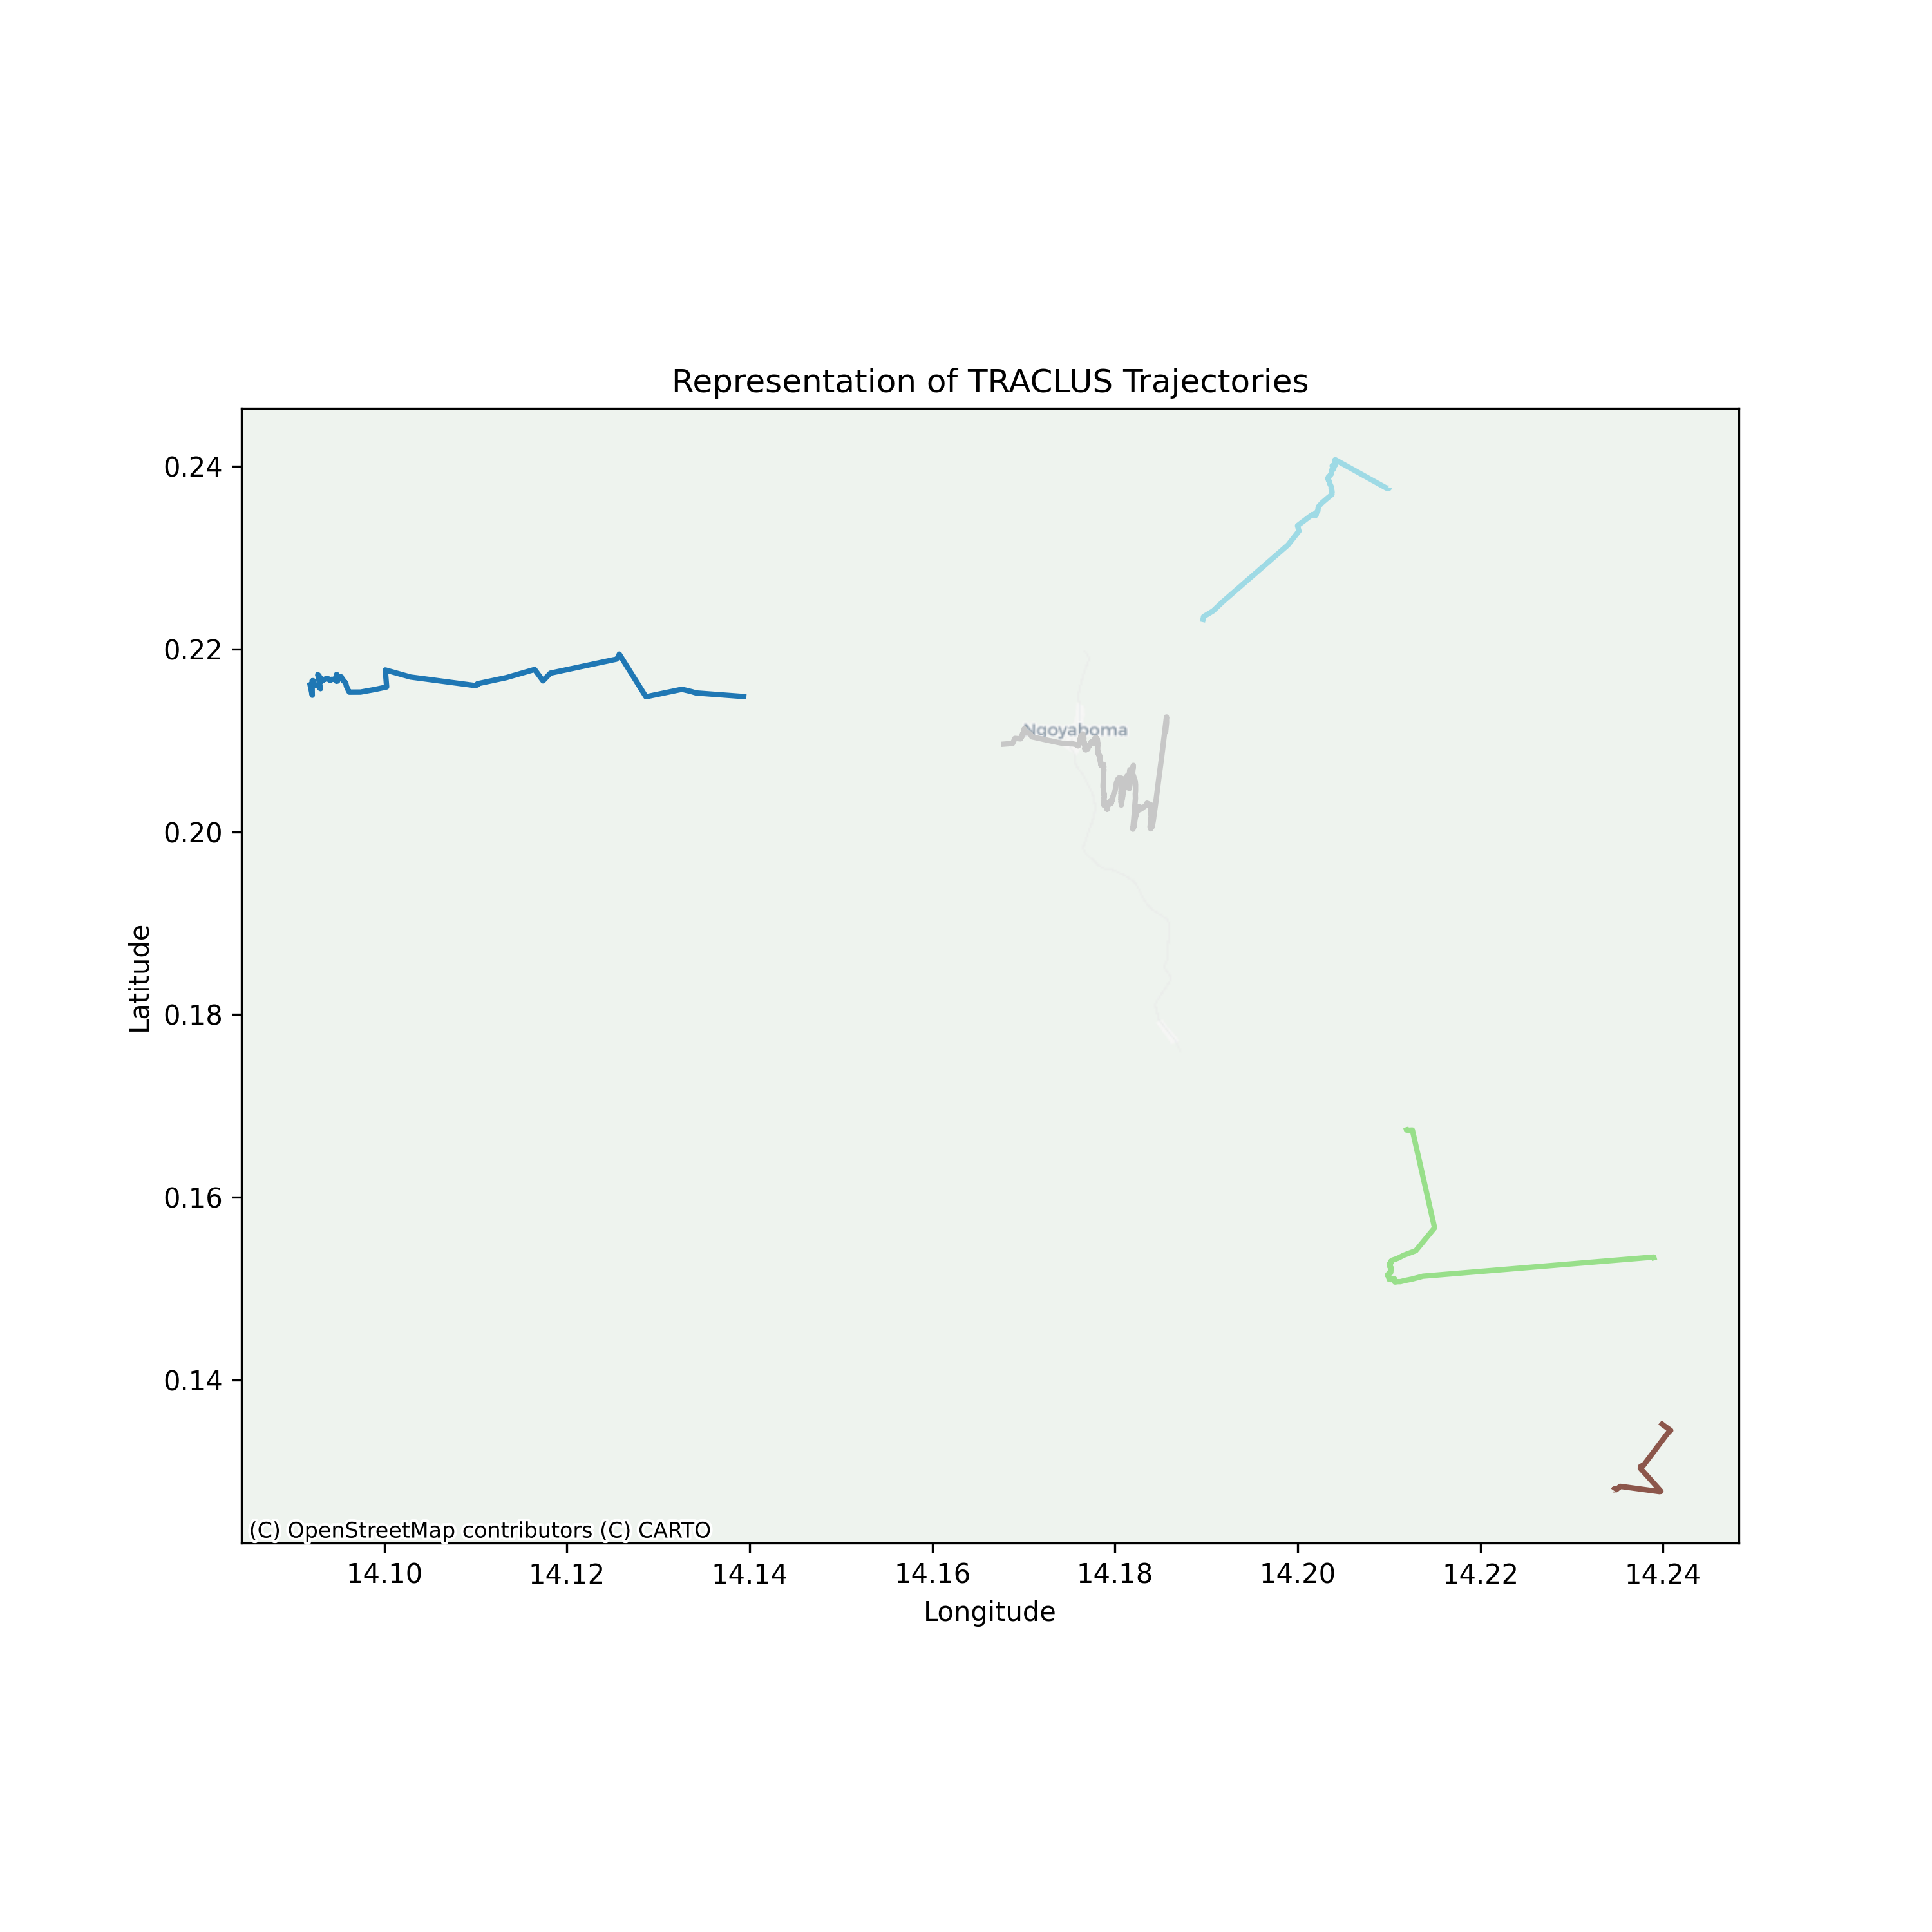
\includegraphics[width=0.5\textwidth]{img/Movebank/map_hdbscan_min.png}
    \caption{Resultados con aumento del $\min_{\text{sample}}$ en HDBSCAN.}
    \label{fig:min_sample}
\end{figure}

\subsubsection{Spectral y Agglomerative Clustering}

Aunque todos los parámetros pueden causar cambios en los resultados en Spectral y Agglomerative el numero de clusters seleccionado en el parámetro mas significativo. Esta cambia absolutamente el resultado y el tiempo de ejecución, cuando se le ponen cantidades bajas respecto a la cantidad de datos analizada los resultados bastante erráticos aunque si se pueden ver las zonas mas pobladas de coordenadas, ademas la transición de clusters a la representación de rutas no toma datos desechables por lo que si se van aumentano los clusters poco a poco el resultado comienza a se mas difícil de analizar, sin embargo llega a un punto en el que el programa comienza a catalogar clusters como desechables y los resutados pasan a ser mas acotados en ocasiones similares a los demas algoritmos o mucho mas pequeños.

\begin{figure}[h!]
    \centering
    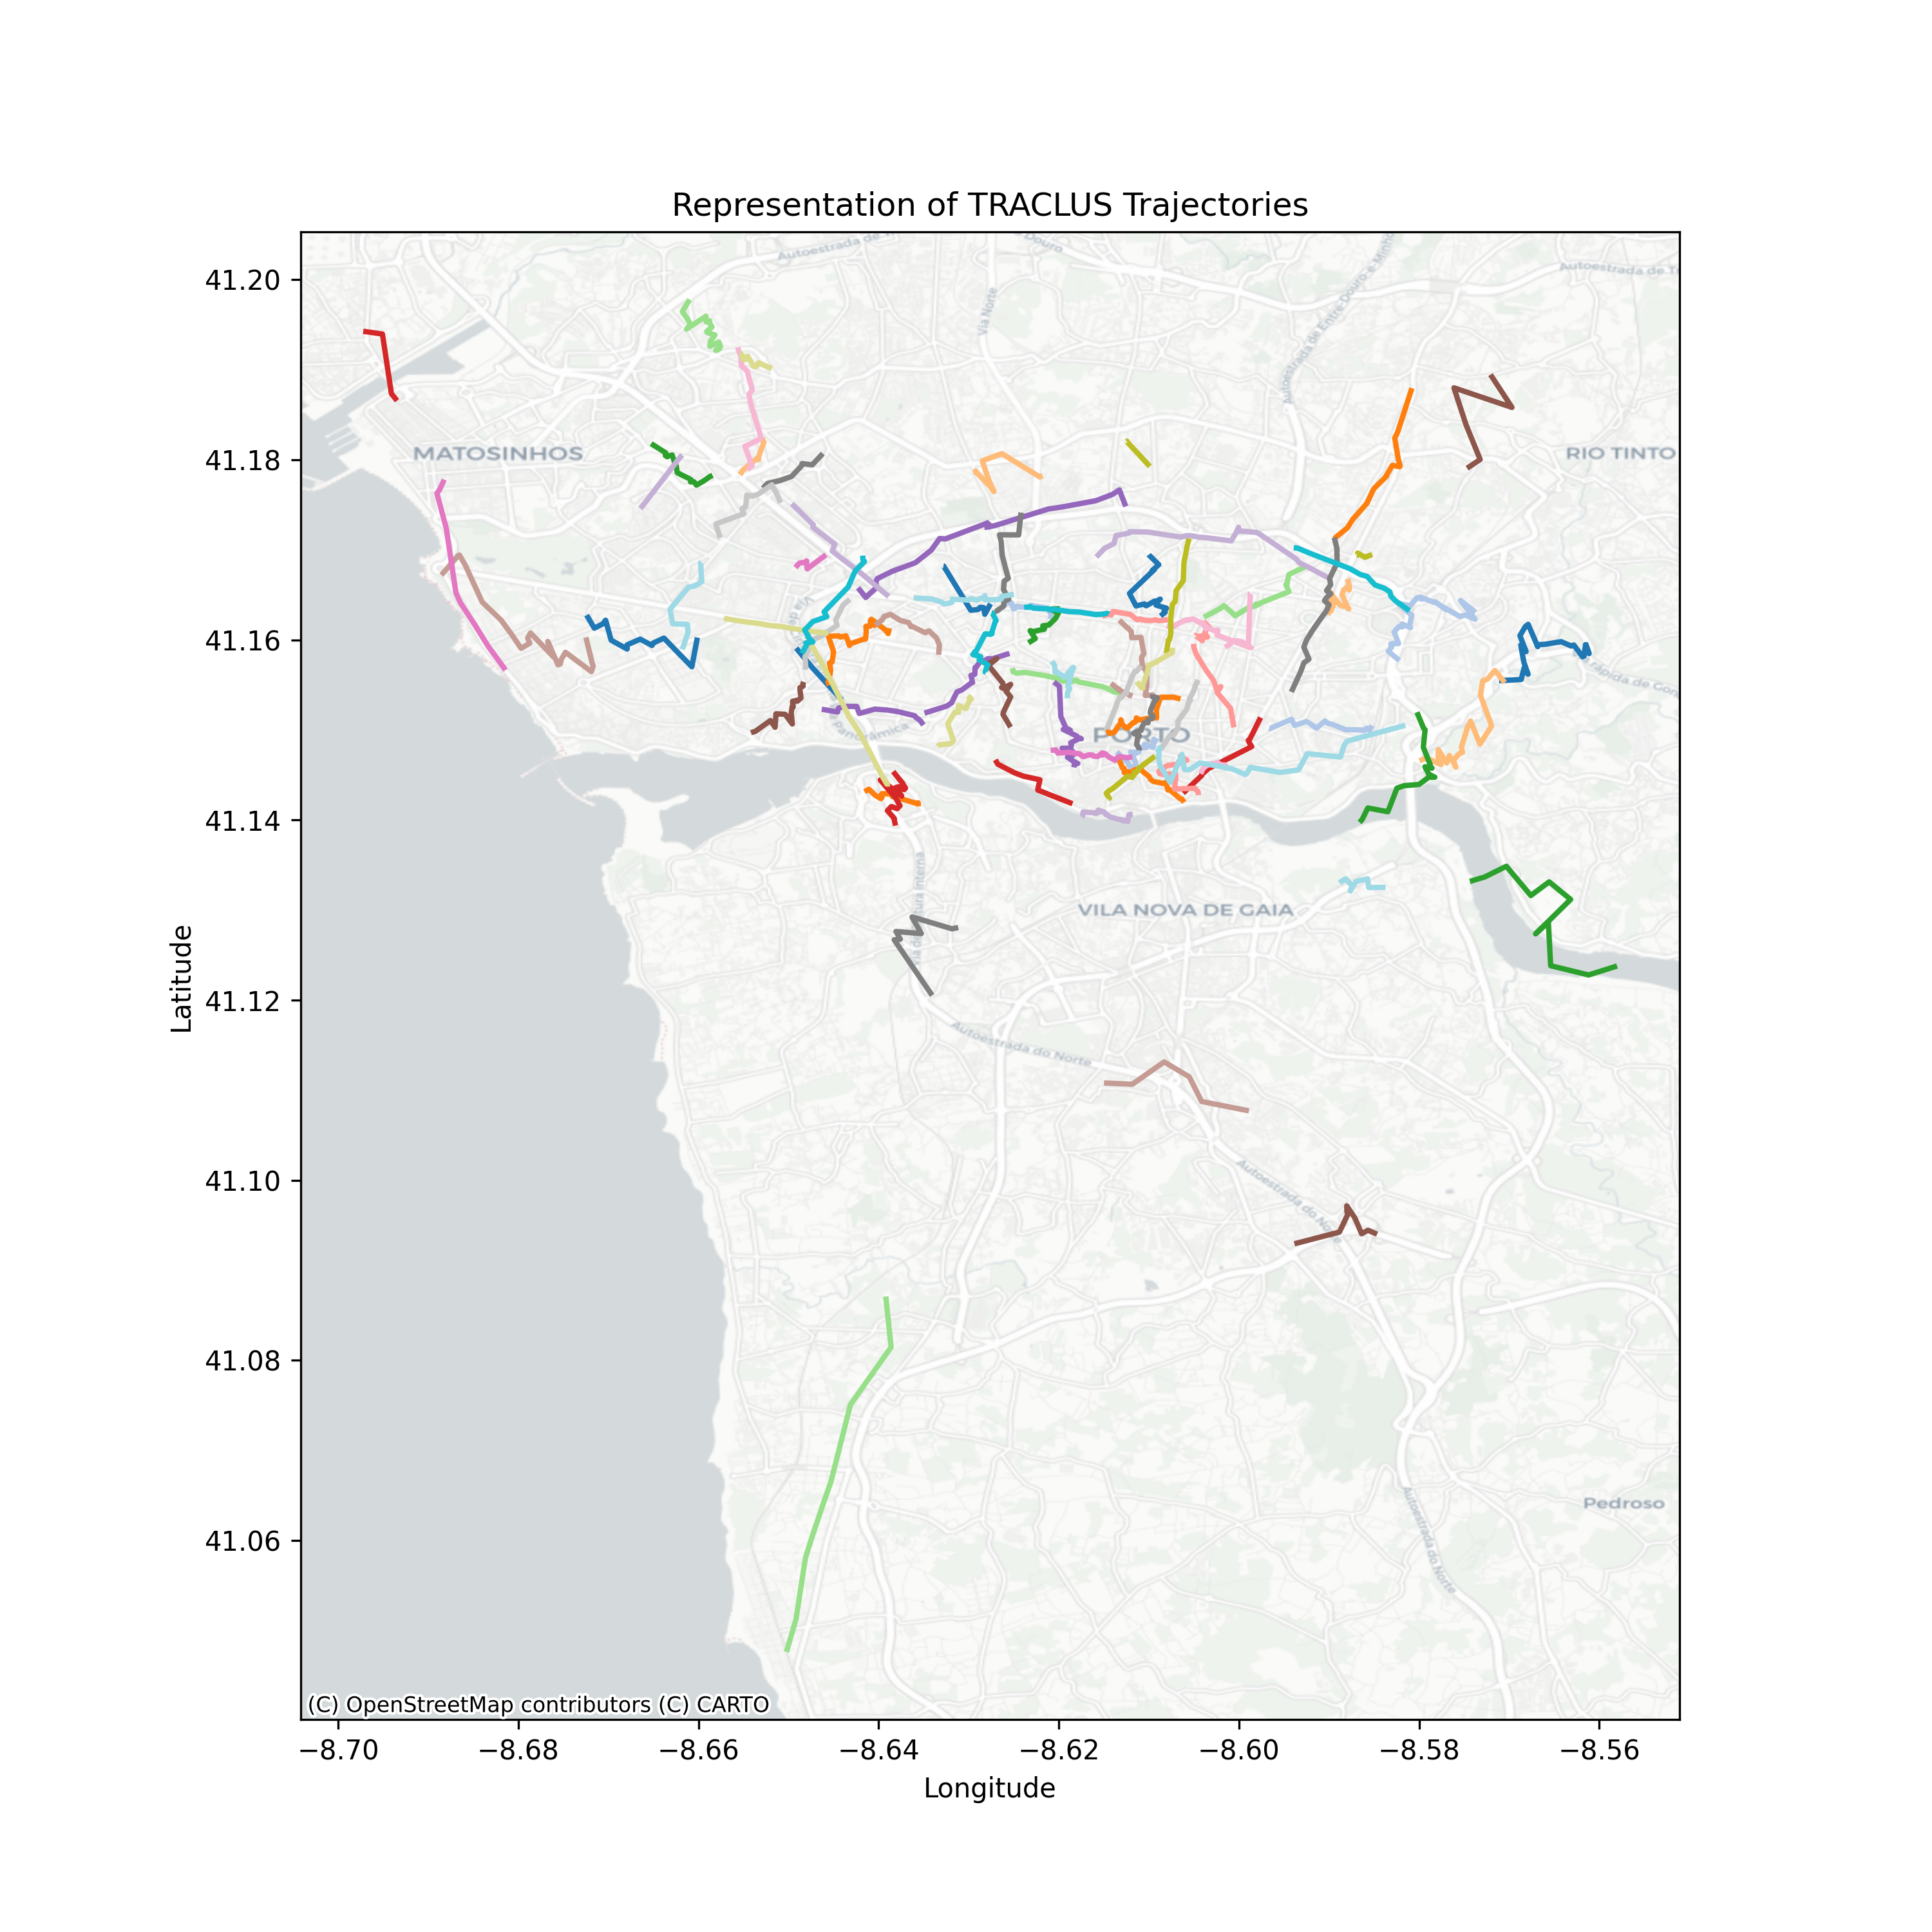
\includegraphics[width=0.5\textwidth]{img/Taxis/map_spect_90.png}
    \caption{Resultados con 90 clusters en Spectral.}
    \label{fig:spectral_90}
\end{figure}

\begin{figure}[h!]
    \centering
    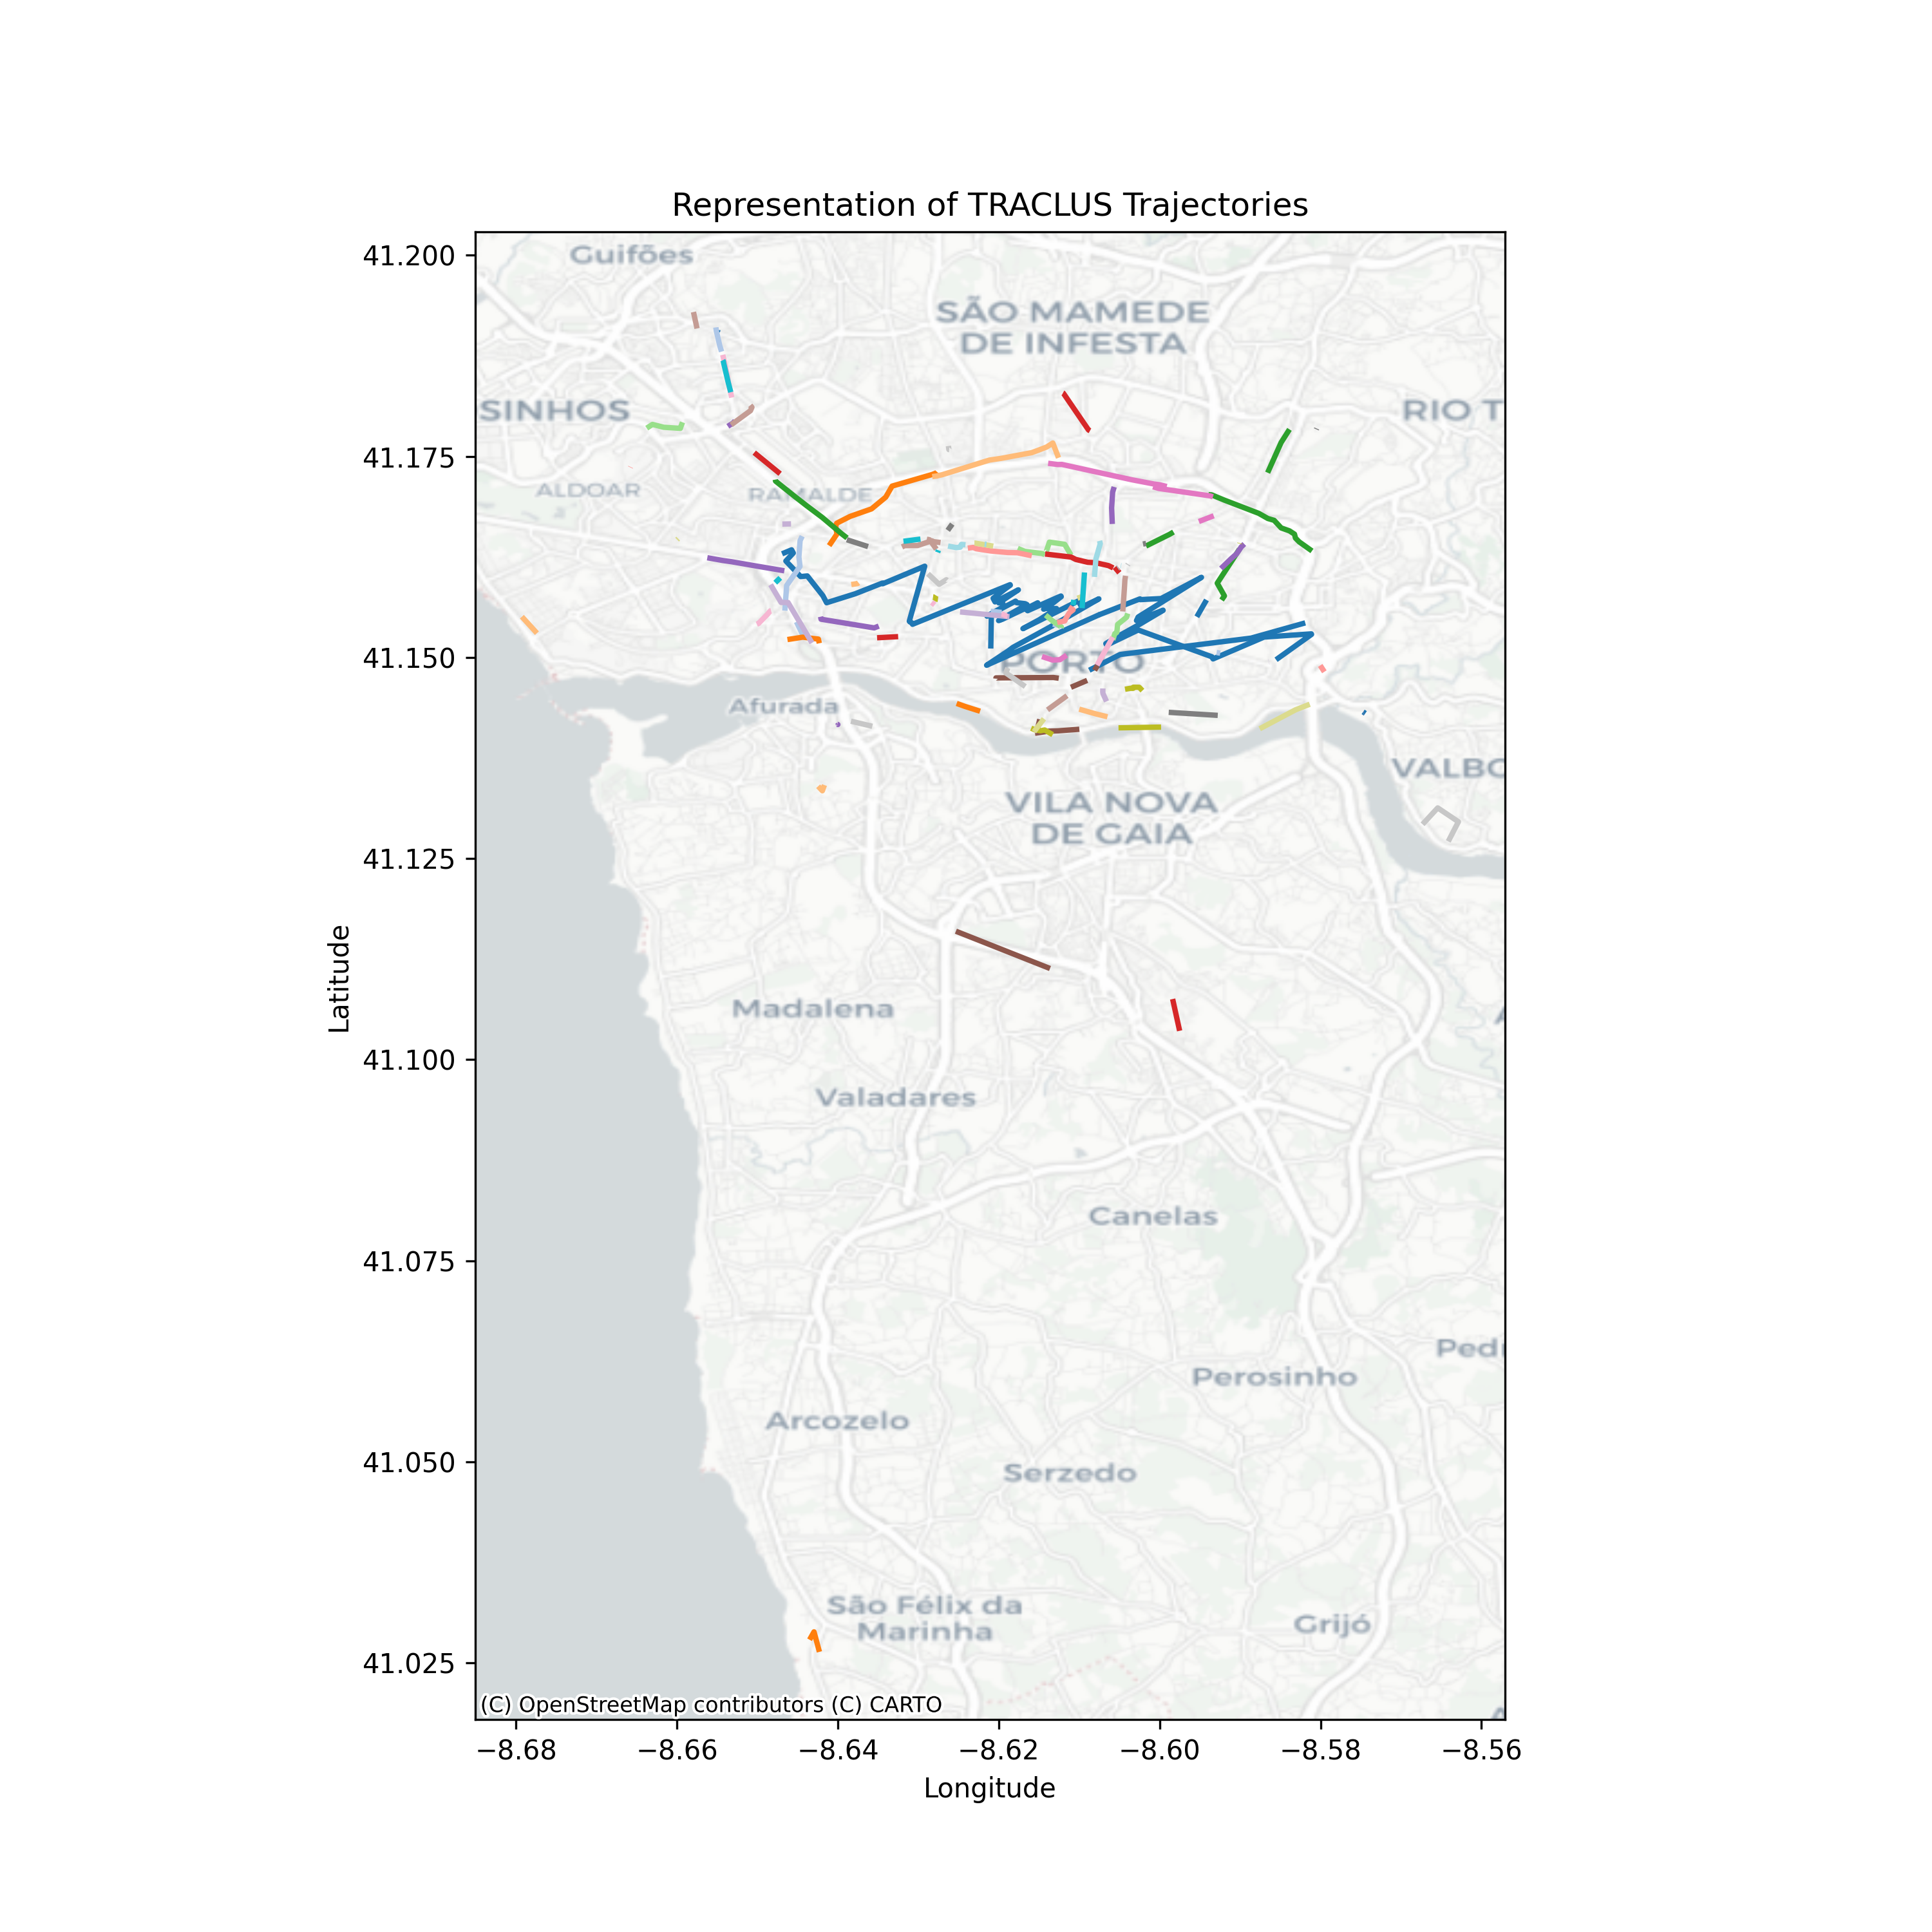
\includegraphics[width=0.5\textwidth]{img/Taxis/map_spect_500.png}
    \caption{Resultados con 500 clustes en Spectral.}
    \label{fig:spetral_500}
\end{figure}

\begin{figure}[h!]
    \centering
    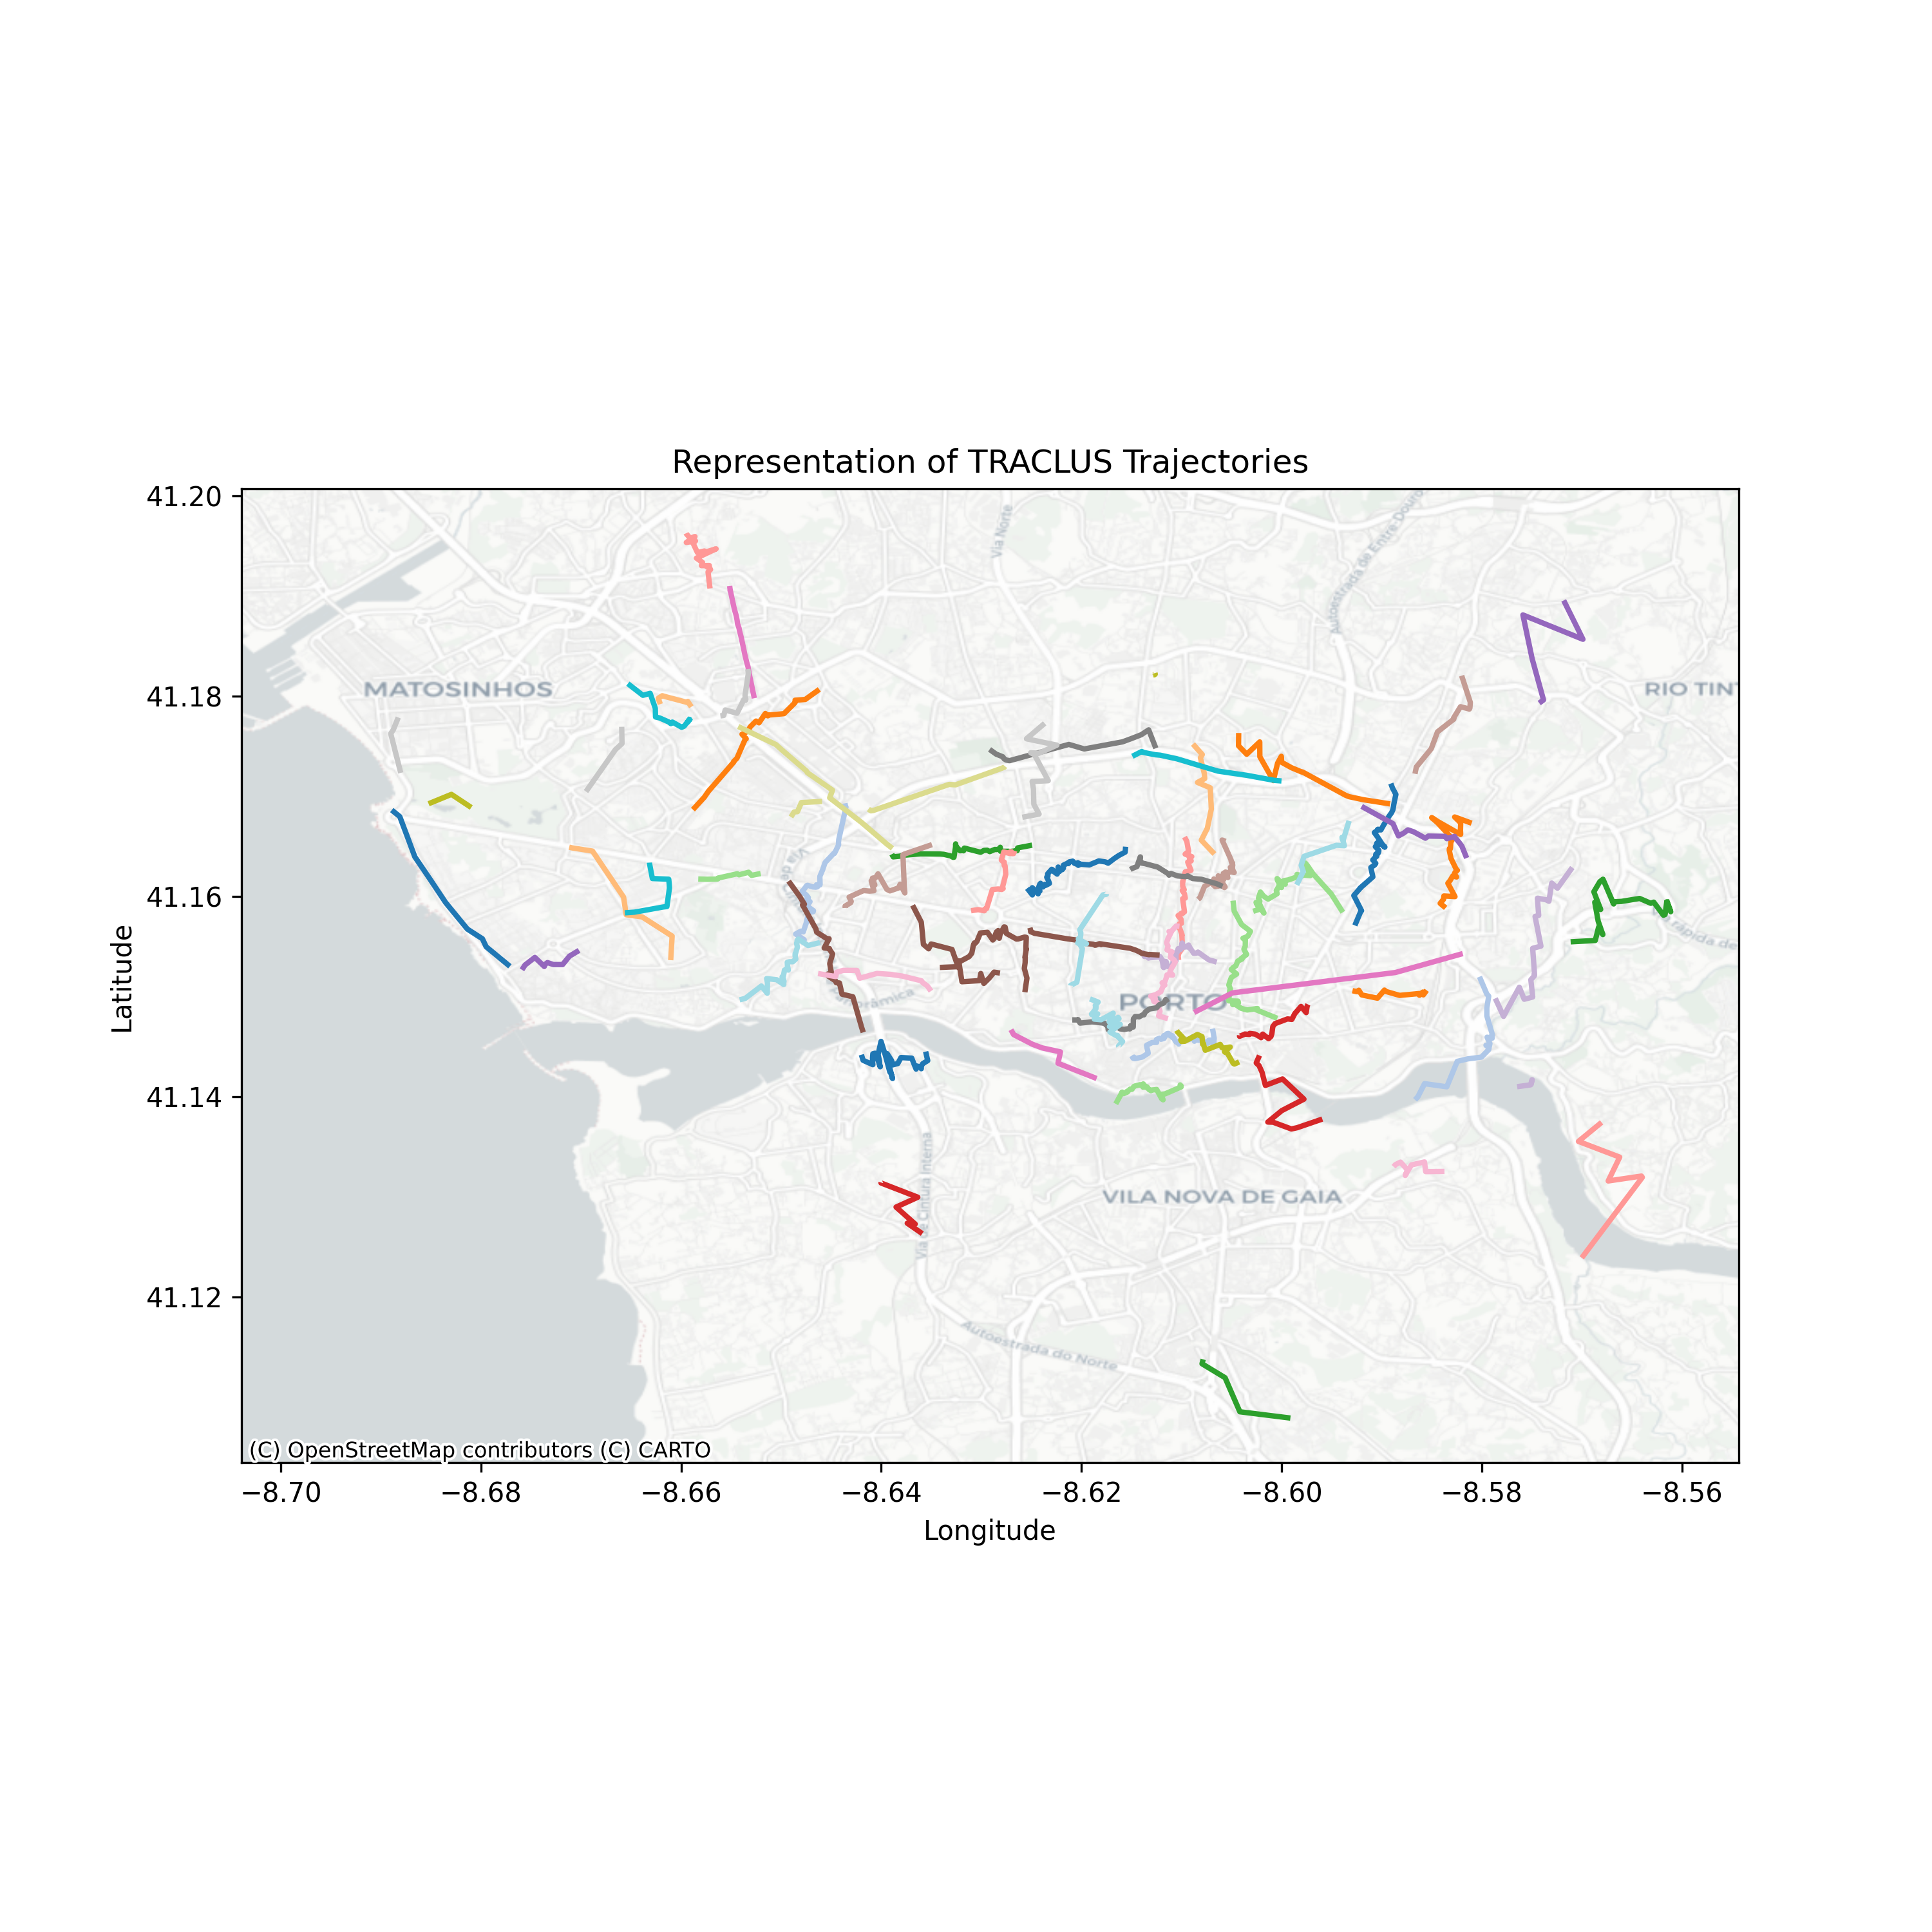
\includegraphics[width=0.5\textwidth]{img/Taxis/map_agglo_90.png}
    \caption{Resultados con 90 clusters en Agglomerative.}
    \label{fig:agglo_90}
\end{figure}

\begin{figure}[h!]
    \centering
    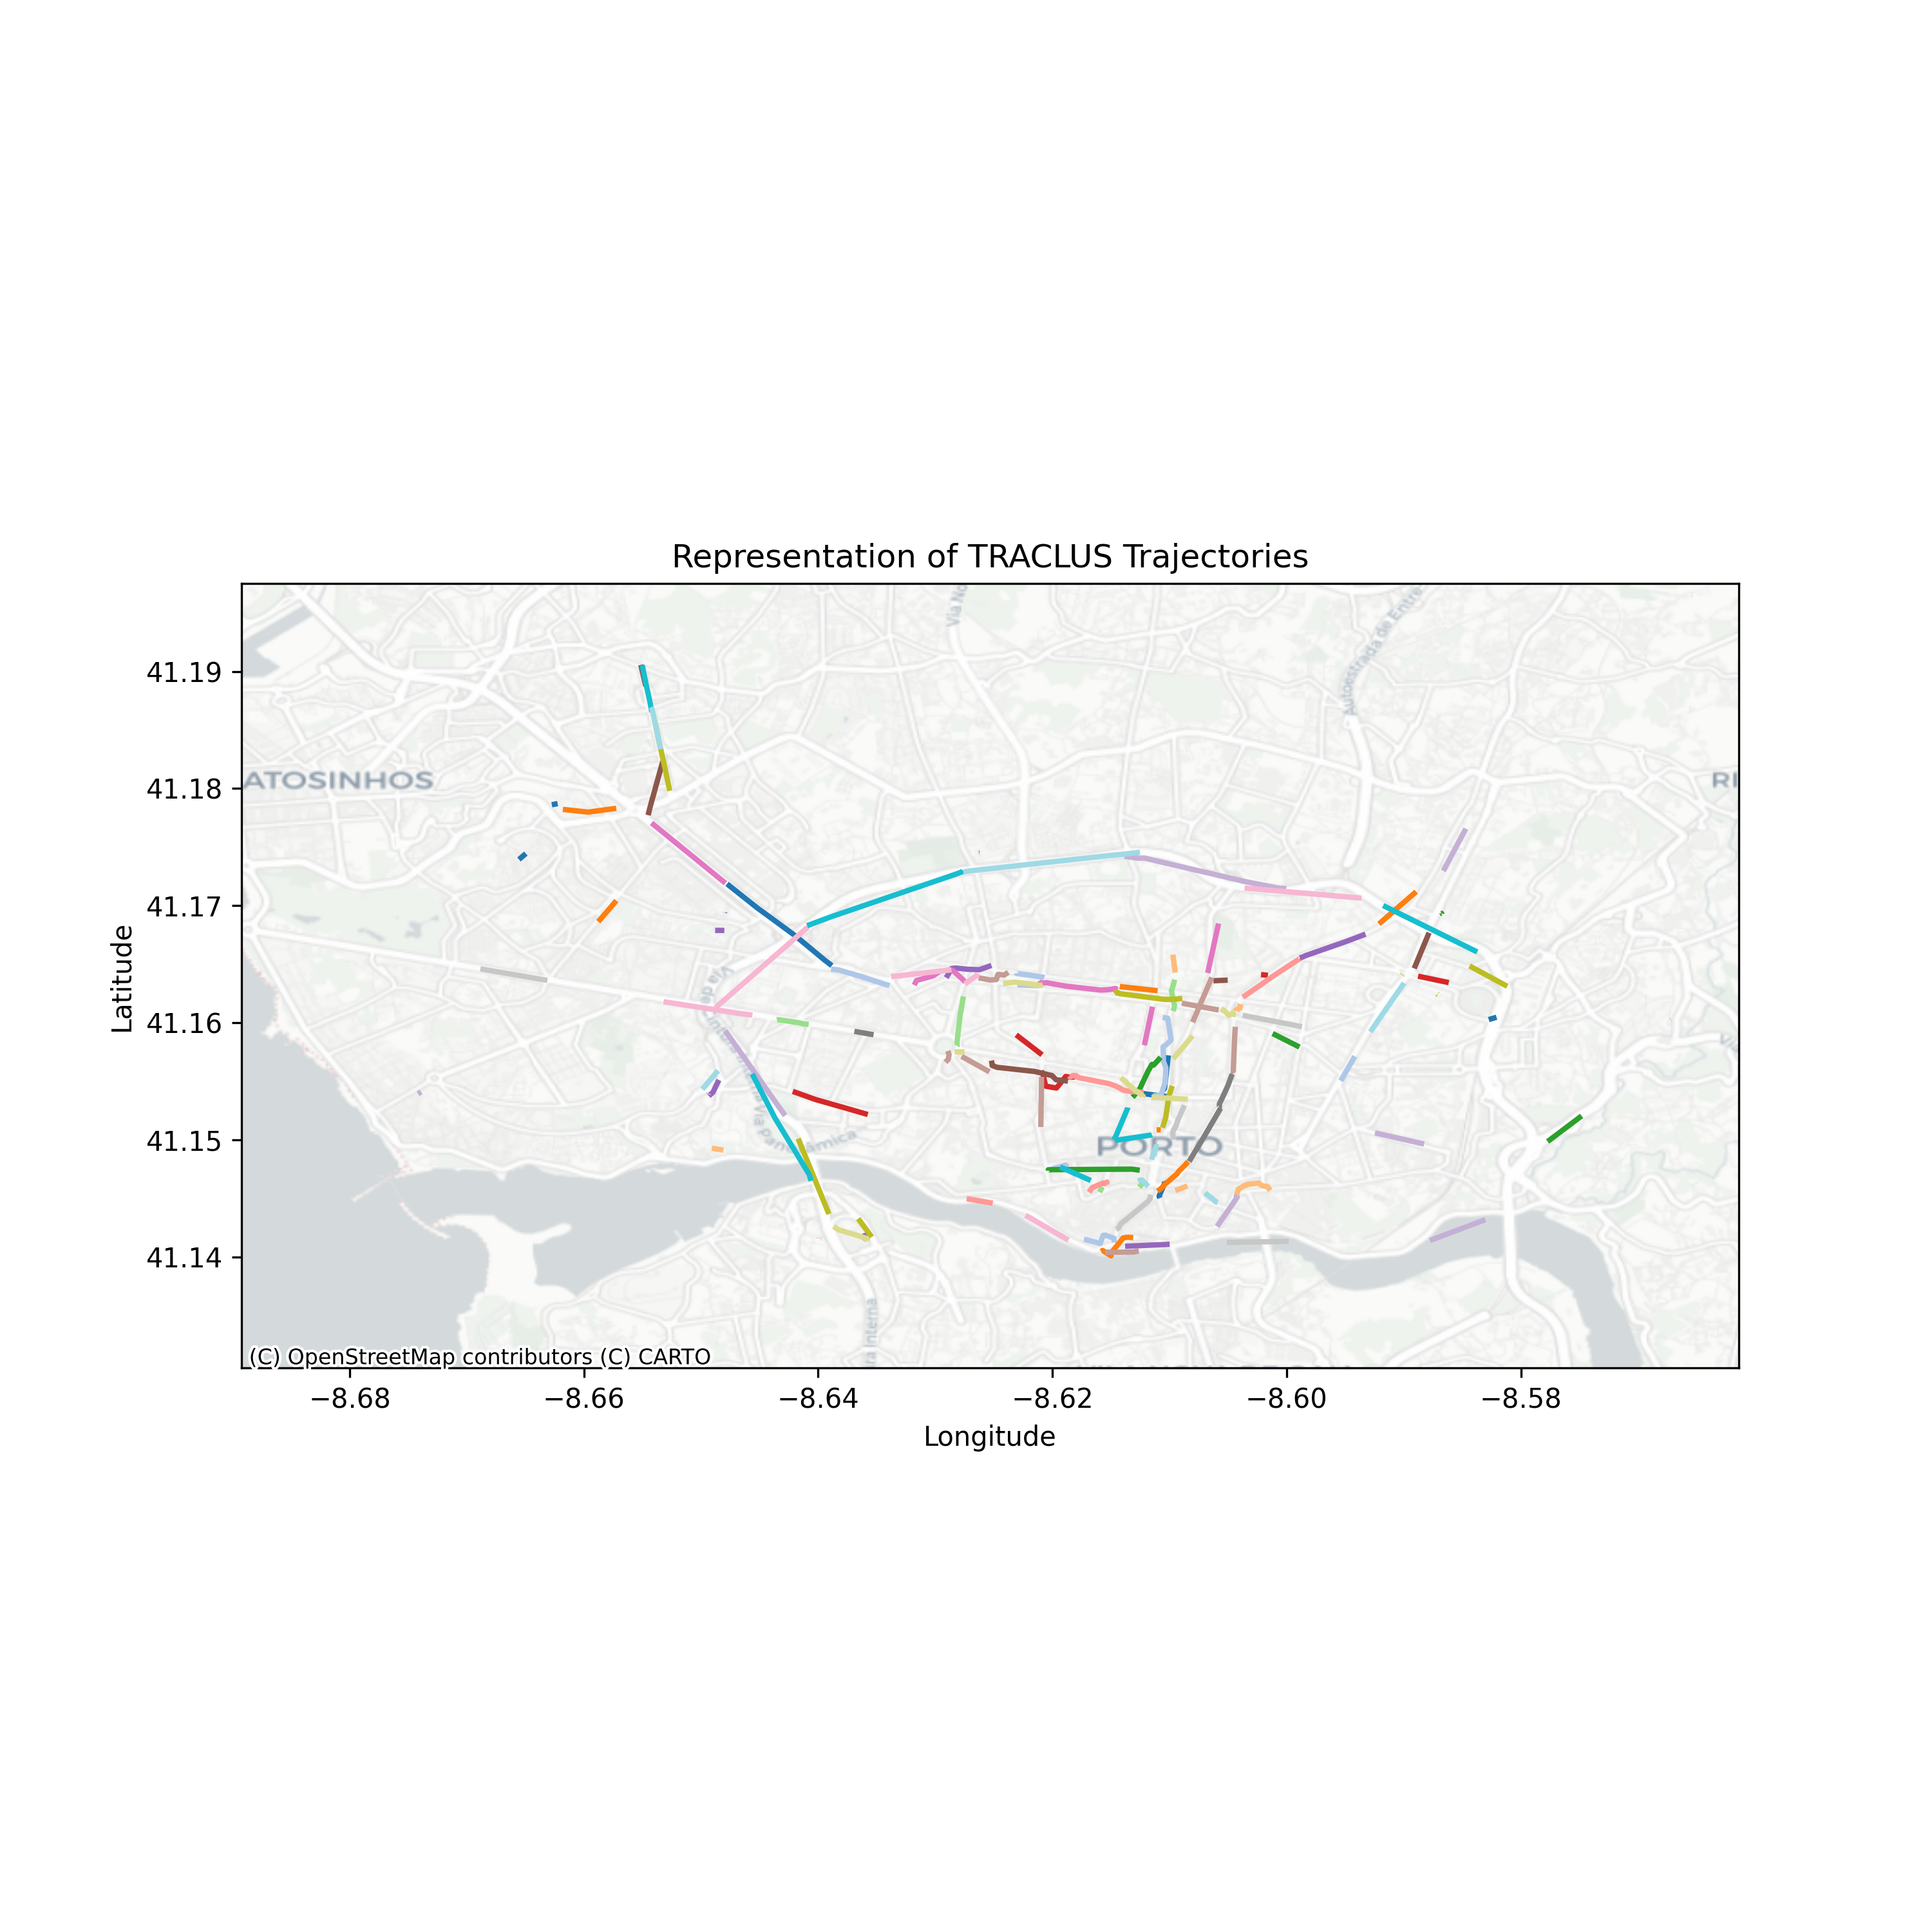
\includegraphics[width=0.5\textwidth]{img/Taxis/map_agglo_500.png}
    \caption{Resultados con 500 clustes en Agglomerative.}
    \label{fig:agglo_500}
\end{figure}

Los otros parametros no se quedan tan atras en modificacion de los resultados. En ambios la agrupecion de los clusters se ve con multiples variaciones llegango ha hacer resultados vastante erraticos.

\begin{figure}[h!]
    \centering
    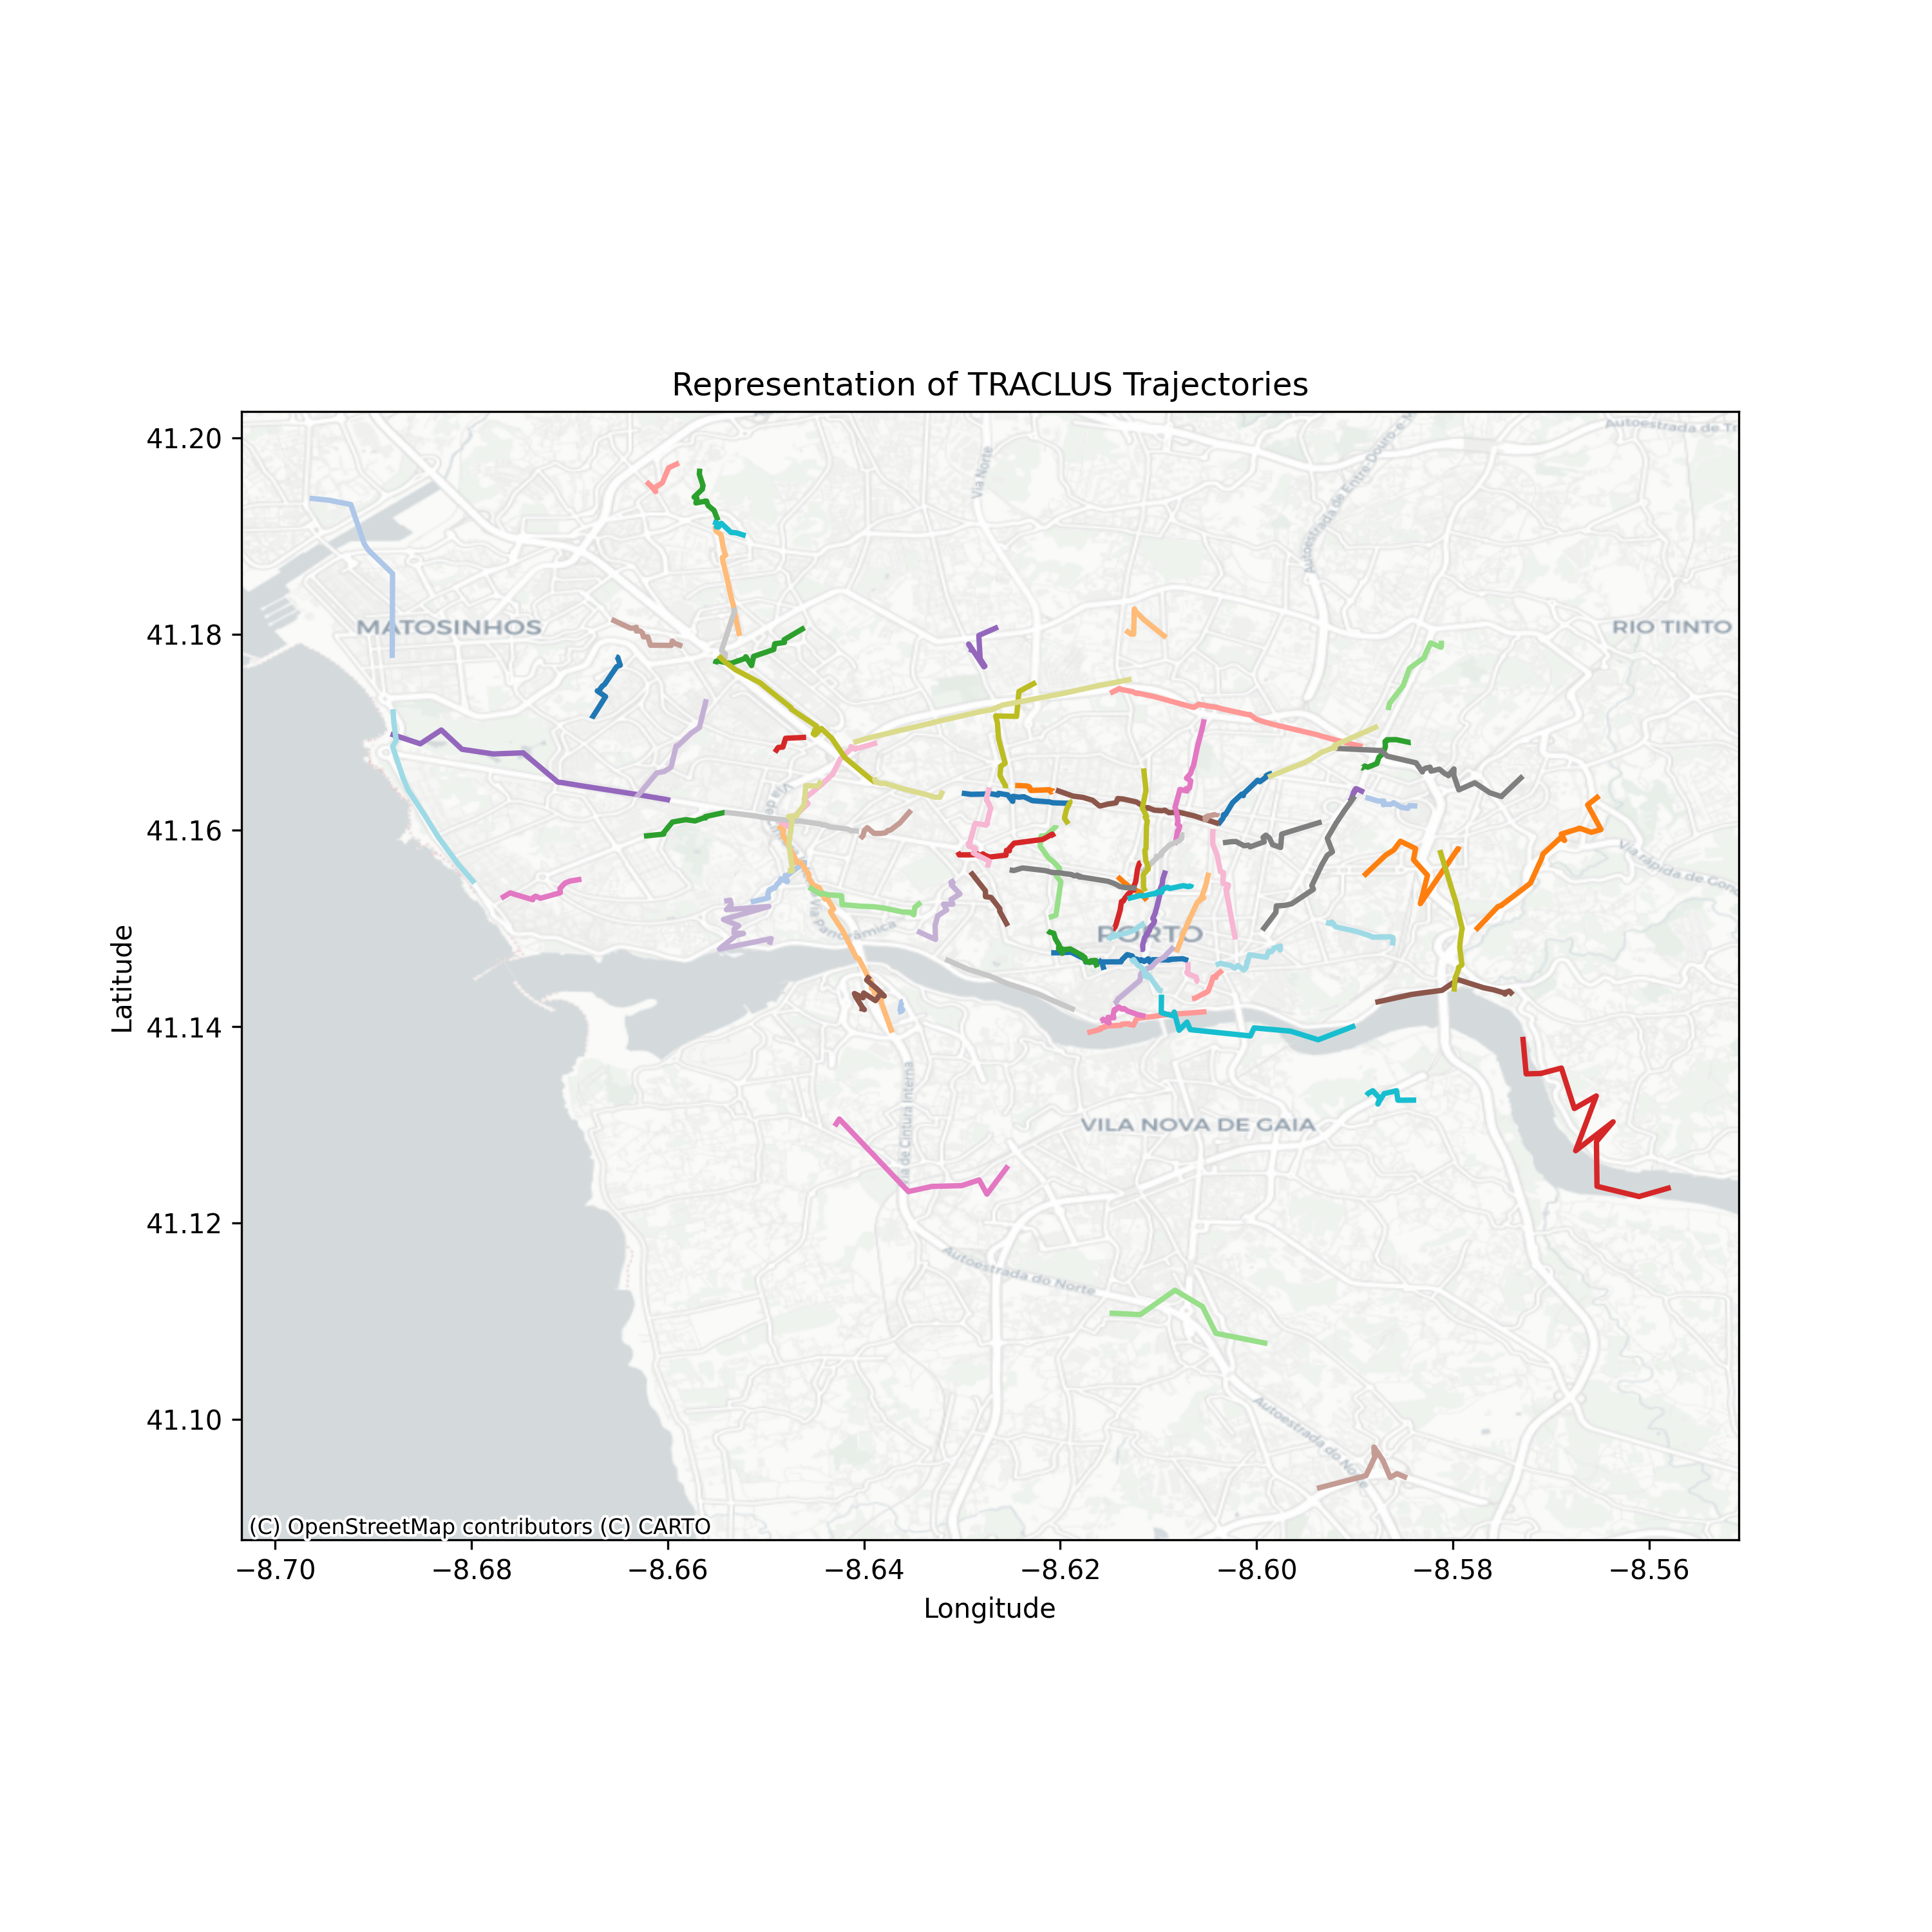
\includegraphics[width=0.5\textwidth]{img/Taxis/map_spect_par.png}
    \caption{Resultados con 90 clusters, $\text{precomputed}_{\text{nearest\_neighbors}}$ y discretize en Spectral.}
    \label{fig:spectal_par}
\end{figure}

\begin{figure}[h!]
    \centering
    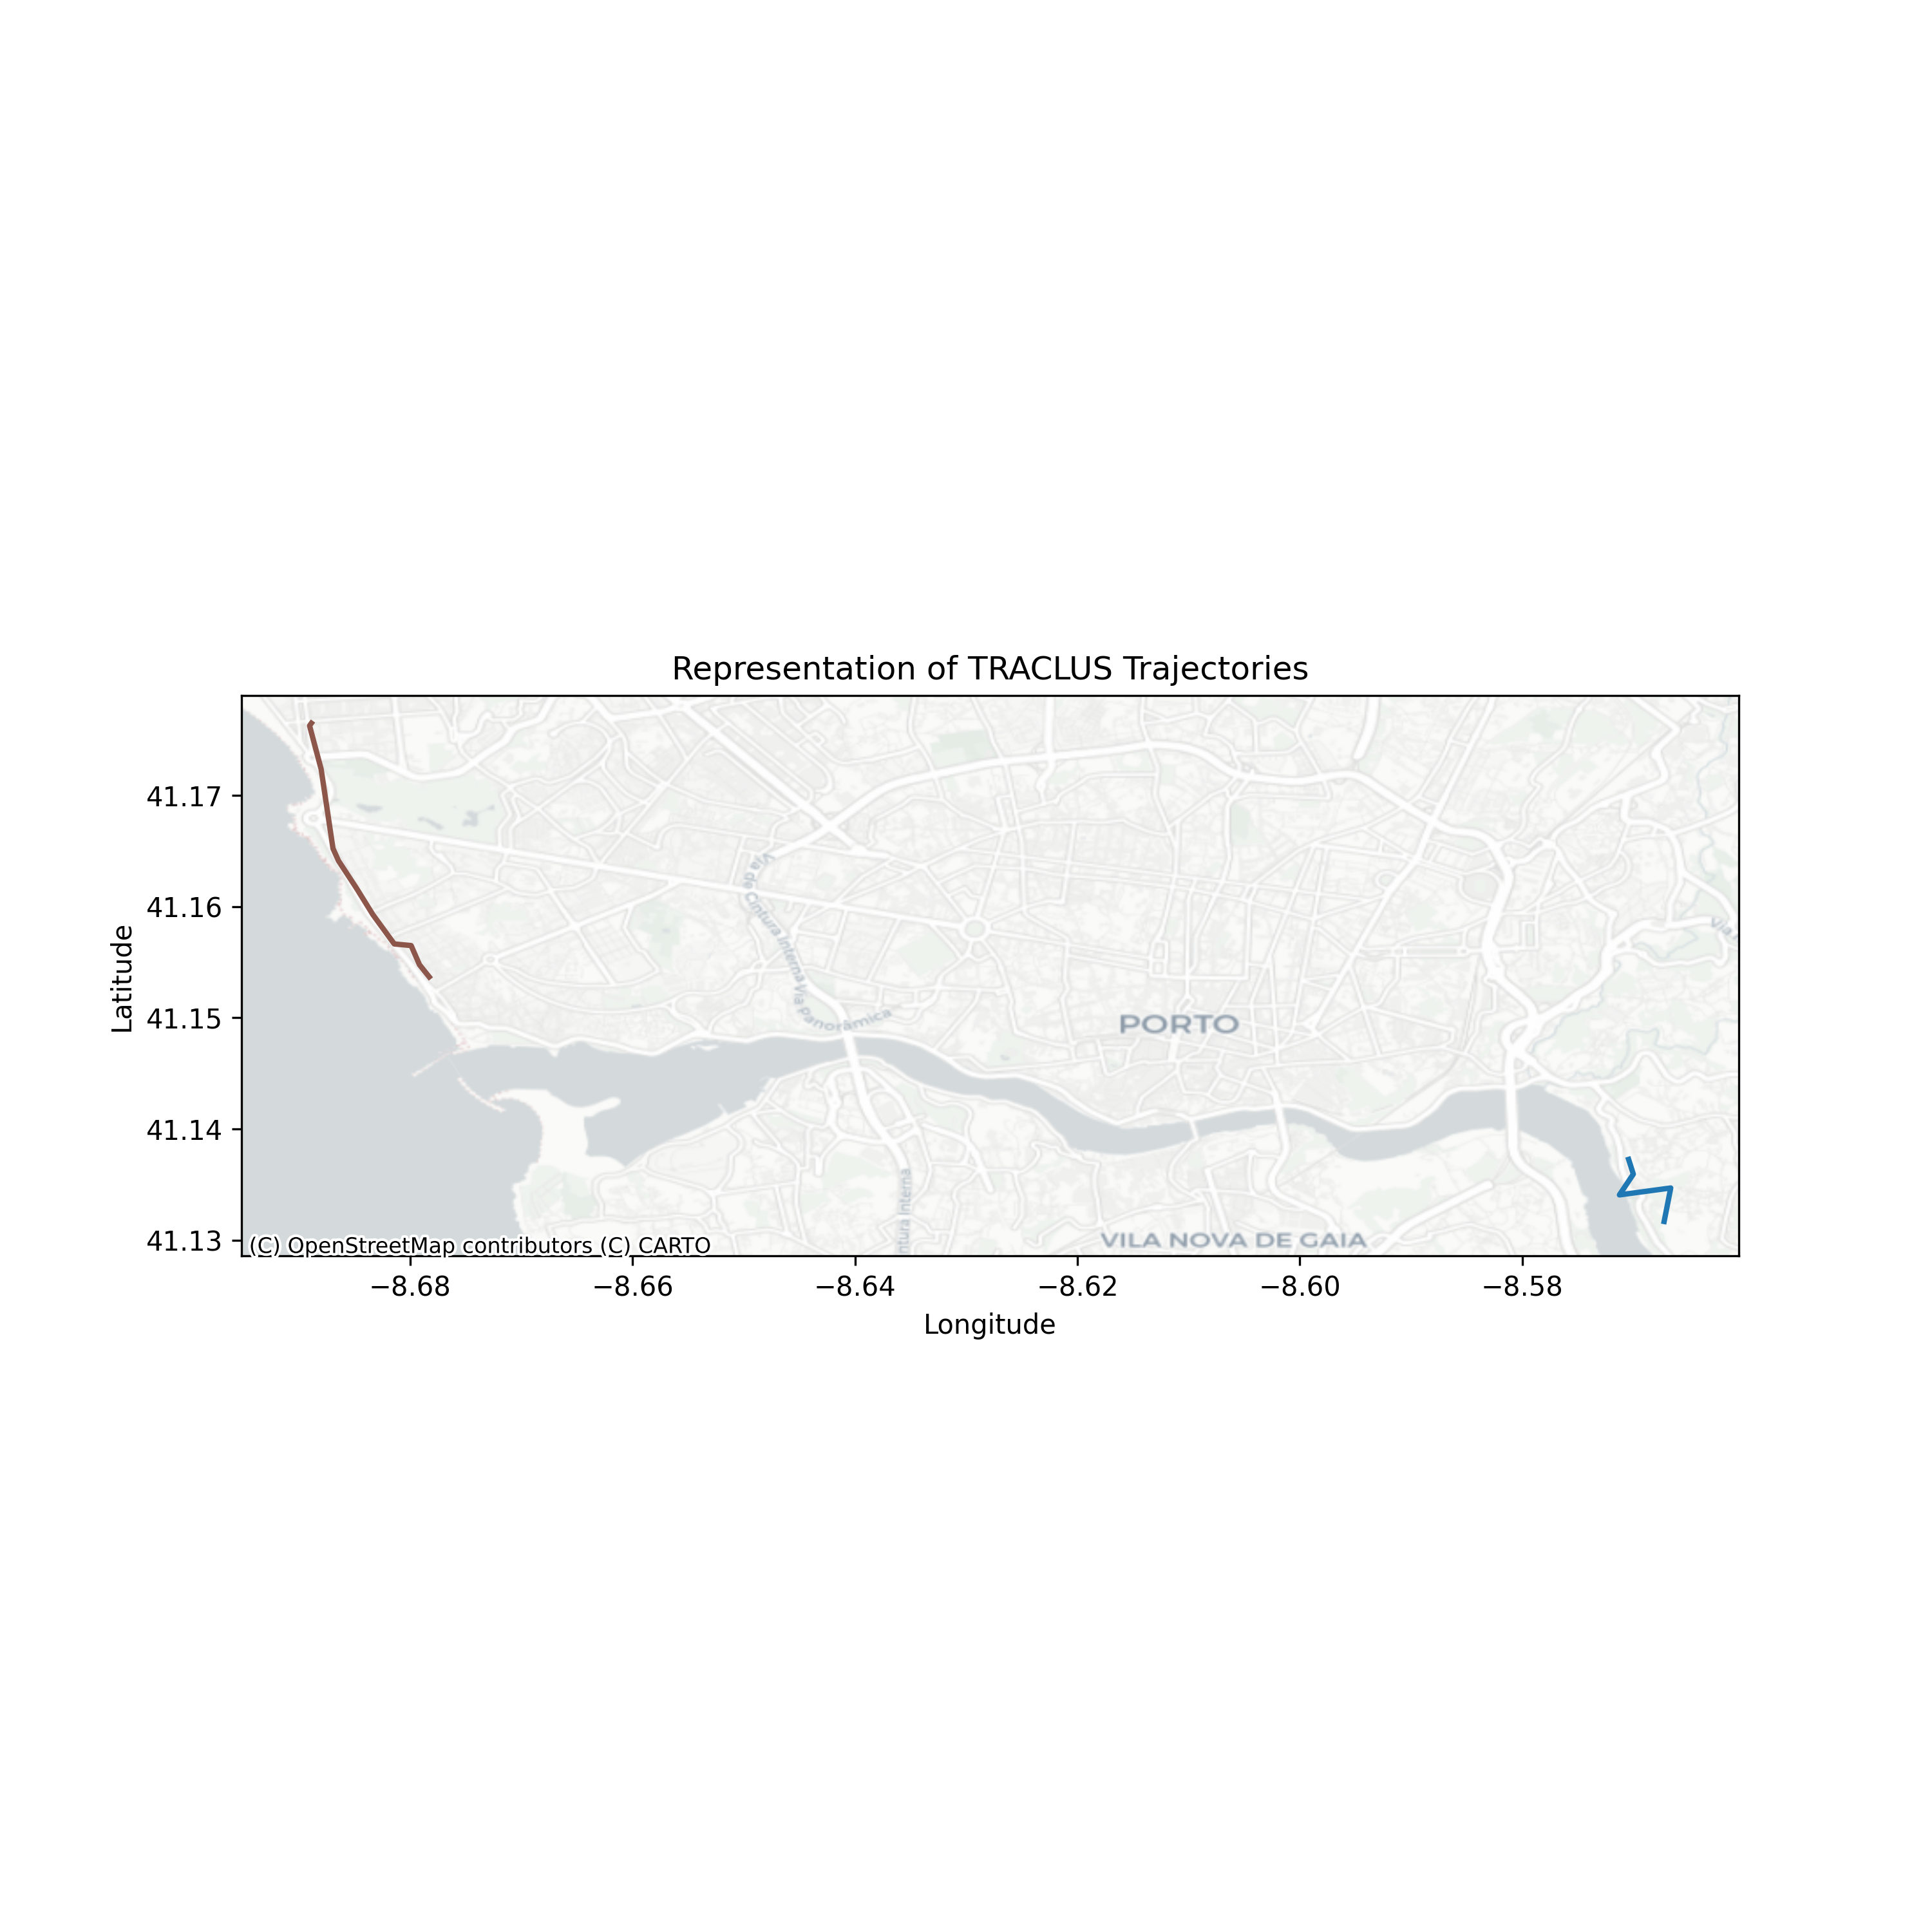
\includegraphics[width=0.5\textwidth]{img/Taxis/map_agglo_par.png}
    \caption{Resultados con 90 clustes y single en Agglomerative.}
    \label{fig:agglo_par}
\end{figure}

\subsection{Conclusión}

Aunque todos los algoritmos analizados muestran cierta utilidad, y aunque se podrían realizar pruebas más exhaustivas y variadas, es posible extraer algunas conclusiones preliminares.

\begin{table}[ht]
\centering
\begin{tabular}{|l|c|c|c|}
\hline
\textbf{Algoritmos} & \textbf{Trayectorias Taxis (seg)} & \textbf{MoveBank (seg)} & \textbf{Geolife (seg)}  \\
\hline
OPTICS & 344 & 766 & 3871 \\
DBSCAN & 327 & 767 & 4048 \\
HDBSCAN & 478 & 865 & 4947 \\
Spectral Clustering & 469 & 928 & 4758 \\
Agglomerative Clustering & 465 & 917 & 4757 \\
\hline
\end{tabular}
\caption{Tiempos de ejecución de los algoritmos en segundos}
\label{tabla:comparacion_algoritmos}
\end{table}

Para aplicaciones en tiempo real o con grandes volúmenes de datos, los algoritmos Spectral y Agglomerative no son recomendables, ya que su tiempo de ejecución aumenta considerablemente. Para obtener resultados más claros, estos métodos requieren un número elevado de clústeres, lo que incrementa aún más el tiempo de procesamiento.

Además, la necesidad de ajustar los parámetros según el tamaño y las características de cada conjunto de datos es otro desafío. En este contexto, HDBSCAN destaca por su versatilidad, dado que determina automáticamente tanto el número como el tamaño de los clústeres. Sin embargo, esta flexibilidad tiene un costo: los resultados fueron en ocasiones poco interpretables, y el tiempo de ejecución superó al de OPTICS y DBSCAN.

Por otro lado, OPTICS demostró ser consistente y eficiente en todos los escenarios evaluados, lo que respalda su elección como algoritmo preferido en las pruebas iniciales.

Finalmente, DBSCAN tiende a crear un número reducido de clústeres, concentrándose principalmente en las regiones de mayor densidad y rechazando segmentos menos poblados. Esta característica, compartida en cierta medida con los algoritmos Spectral y Agglomerative, se manifiesta de manera opuesta: mientras DBSCAN agrupa solo las áreas más densas, Spectral y Agglomerative distribuyen clústeres de manera amplia, pero con una representatividad reducida a medida que aumenta su número.











